\documentclass[a4paper,12pt]{article}
\usepackage[dvipsnames]{xcolor}
\usepackage{etoolbox} \usepackage[english]{babel} \usepackage[utf8]{inputenc} \usepackage{amsmath} \usepackage{amsfonts} \usepackage{amsthm} \usepackage{graphicx} \usepackage[colorinlistoftodos]{todonotes} \usepackage{amsfonts} \usepackage{bbm} 
\usepackage{setspace} 
\usepackage{enumitem}
\usepackage{pdfsync} \usepackage{xr}
\usepackage[ruled]{algorithm2e}
\usepackage{tikz}
\usepackage{caption}
\usepackage{subcaption}
\usepackage[margin=0.9in]{geometry}
\usepackage{comment}
% \usepackage{authblk} % NEW!!!
% \bibliographystyle{econometrica}

\bibliographystyle{plainnat}
\usepackage{hyperref}       % hyperlinks
\hypersetup{
    colorlinks=True,
    citecolor=blue,
    linkcolor=blue,
    filecolor=blue,      
    urlcolor=blue,
    pdftitle={RFP},
    pdfpagemode=FullScreen,
    }

\usepackage{natbib}

\newtheorem{theorem}{Theorem}[section] \newtheorem{proposition}{Proposition}[section] \newtheorem{lemma}{Lemma}[section]

% \newtheorem{definition}{Definition}[section]
\newtheorem{example}{Example} \newtheorem{corollary}{Corollary}[section] \newtheorem{remark}{Remark}[section] \newtheorem{assumption}{Assumption} \newcommand{\citeposs}[1]{\citeauthor{#1}'s \citeyearpar{#1}} \newcommand\fnote[1]{\captionsetup{font=small}\caption*{#1}}

%\usepackage[a4paper,left=3cm,width=14cm,right=3cm]{geometry}
%\def\qed{\rule{2mm}{2mm}} \parskip = 1.5ex
%\textwidth 7in
%\textheight 10 in
%\oddsidemargin -0.4 in
%\evensidemargin -0.4in
%\topmargin -0.7in
\setlength{\parindent}{2em}
\setlength{\parskip}{0.5em}
\renewcommand{\baselinestretch}{1.15}




\begin{document}


\begin{titlepage}
\title{A Deep Learning Assessment of the Right to Counsel}
%\shortTitle{Short title for running head}

\author{Patrick Power, Shomik Ghosh and Markus Schwedeler \\ 
\textcolor{red}{DRAFT}}
\date{\today}
\maketitle
\thispagestyle{empty} % makes the title page number not appear
\vspace{-2em}
\begin{abstract}
Drawing from the Deep Learning Literature and in the language of Category Theory, we introduce a unified estimation framework that generalizes ordinary least squares, allows for nonparametric cluster effects,\footnote{To clarify this point, in many applied microeconomic contexts, individuals grouped together in some fashion. In our context, this grouping is done via a shared zip code. We indicate this grouping via an indicator variable. The nonparametric component is that we allow these the effect of this group memebership on the outcome of interest to vary across the other controls/features. That is, we don't place a functional form assumption on the way the cluster indicator variable interacts with the other controls.} and is inherently compositional, even under regularization. With this framework, we examine the effects of the Right to Counsel: a policy which ensures that low-income households facing eviction have access to free legal representation. Specifically, we consider the extent to which the policy increases housing instability by making it harder for low-income households to secure housing in the first place. Exploiting the ongoing roll-out of the policy across the state of Connecticut, our preliminary results suggest that housing is harder to secure in areas with higher eviction rates, indicating that the policy is less effective at scale than generally understood. 
\vspace{0.2in}\\
\noindent\textbf{Keywords:} Right to Counsel, Evictions, Deep Learning\\
%\noindent\textbf{JEL Codes:} key1, key2, key3\\
\end{abstract}
\setcounter{page}{1}
\end{titlepage}

%\thispagestyle{empty}

%\pagebreak \newpage


%\oneandhalfspacing
In this paper, the term \textit{Right to Counsel} refers to a policy initiative which ensures that tenants have access to free legal representation in eviction cases. 

\section{Introduction}
The 2 million evictions that occur each year across the United States are costly to individuals, landlords, courts, and the general public. Unlike criminal cases in the U.S., defendants in an eviction case are not entitled to a public attorney. A gap in legal representation, therefore, exists between landlords and tenants which is as large as $95\%-1\%$ in some areas in favor of the landlord  (\cite{collinson2022eviction}). Given the severity of the costs associated with eviction, the multitude of factors which contribute to its occurrence, and the typical manner in which a eviction case is settled, many in the U.S. believe that legal counsel should be provided to low income households. Over the past five years, $15$ cities and $3$ states have introduced a Right to Counsel with the aim of closing this gap and with the hope that doing so will improve downstream outcomes.\par 

To some extent, this hope has been empirically justified when considering the direct outcomes of eviction cases. Both in the context of small scale randomized control trials as well as in city-wide roll-outs, researchers have generally found positive results (\cite{seron2001impact, greiner2012limits, cassidy2022effects}). The pressing unknown, though, is whether the indirect effects associated with the policy diminish or outweigh these positive legal outcomes. To date, one of the most consistent findings is that Legal Aid increases the length of the eviction process.\footnote{\cite{cassidy2022effects} writes: ``The number of days between a case filing and a judgment is also significantly longer in the UA zip codes after program implementation.''} By increasing the cost of evicting a tenant, the policy may disincentive landlords from renting to low-income households in the first place. As \cite{gunn1995eviction} writes, ``By increasing landlords' costs of doing business, legal services attorneys may enrich their clients at the expense of all other similarly situated poor tenants." \par 
In this paper, we draw on recent advances in deep learning to empirically assess whether this concern is justified. Specifically, we use the ongoing rollout of the Right to Counsel across the state of Connecticut to estimate its effect on the ease with which low-income households, who are currently experiencing homelessness, are able to find housing. A key challenge in our setting is that the treatment (the policy) is assigned a level (the zip code) above the unit of interest (the individual). Building on recent deep learning papers (\cite{finn2017model} and \cite{kelly2020learning}), we implement an estimation framework that allows us to partial out the zip code effects in a nonparametric fashion.

While preliminary, our results suggest that across zip codes with a high eviction rate (as measured in 2019), the length of the housing search increases in response to the policy. Using a 30-day threshold, the probability that a household is still searching for housing after this cutoff increases by 5 percentage points. While the sign of this effect is relatively constant across a range of estimators, we emphasize that there are several important concerns/issues that cannot be addressed in our context. This paper should be therefore be understood as the first empirical microeconomic work to consider the unintended consequences of this policy, but given the importance of this topic, it certainly should not be the last.

There are two distinct reasons for why there has been little empirical work on this issue previously. As \cite{abramson2021welfare} notes, there hasn't been a suitable context to empirically assess the indirect effects of the policy. Prior works on the Right to Counsel either focus on small scale randomized control trials, such as (\cite{greiner2012limits}, \cite{seron2001impact}), which by construction only allow for the study of direct outcomes, or as in the case of (\cite{cassidy2022effects} and \cite{ellen2021lawyers}) study the city wide roll-out of New York City which is a very unique housing market.\footnote{\cite{evans2019reducing} writes, ``Not all areas have experienced a decline in homelessness. The trends in New York City (CoC NY600) and Los Angeles County have been particularly different from the rest of the country \dots Note that since 2012, these rates have increased by 57 and 31 percent, respectively.''} Tackling a similar research question to ours, but written one year prior,  \cite{abramson2021welfare} resorts to studying the effects of the Right to Counsel via a counterfactual analysis.\footnote{As \cite{abramson2021welfare} writes, ``I quantify the model to match data on evictions, homelessness, and rents in San Diego
County, and use it for counterfactual analysis.''}\par Only within the past year, as Washington and Connecticut adopted the Right to Counsel at the state level has the possibility of empirically assessing the policy at scale emerged. And only in the case of Connecticut, which adopted a meaningful and well documented staggered roll-out has this opportunity been realized. Due to supply constraints of legal services, low-income individuals in only a subset of Connecticut zip codes currently receive free legal aid under the policy. Meaningfully for our paper, several high eviction rate zip codes remain untreated as highlighted in figure \ref{fig:efr}.\par 

The second reason this topic remains understudied is that the indirect effects of the Right to Counsel are difficult to capture. Evictions themselves are often informal. Mathew Desmond writes in his New York Times Best Seller, \textit{Evicted}, that informal evictions in Milwaukee account for $48\%$ of forced moves while formal evictions account for $24\%$. It seems reasonable to expect landlords to respond to the Right to Counsel through a number of informal or hard to detect ways. Indeed. from conversations with lawyers who specialize in evictions, the question at times seemed not to be whether the costs of the Right to Counsel would be passed on to the tenants, but rather whether they would be observable in the data. As one lawyer explained,  ``The thing to remember is that higher costs for landlords always get passed on to the tenants in some form (higher rent, deposits, fees, etc.)."\par 
To empirically assess the roll-out of the policy across the state of Connecticut, we therefore make use of individual level data related to local Rapid Rehousing Programs within the state. Tracked by the U.S. Department of Housing and Urban Development, theses programs assist households experiencing homelessness secure housing. Importantly for our work, these programs (1) are restricted to households who don't face significant barriers to housing, (2) provide limited short-term financial assistance and (3) require that the rental agreements that households sign have ``the same rights and responsibilities as a typical lease holder.''\footnote{\href{thttps://endhomelessness.org/resource/rapid-re-housing-a-history-and-core-components/}{Reference}: ``It is imperative that any lease agreement provides the tenant with **the same rights and responsibilities as a typical lease holder** and that the financial terms of the lease are such that the household has a reasonable ability to assume rental costs once financial support ends (keeping in mind that in the majority of cases, even households with no income at move-in retain their housing)"} For each household, we observe both pre-treatment characteristics (race, gender, family structure) as well as their length of their housing search, which is the main outcome variable of interest. \par 
To this data set, we fit a series of estimators all within a single, unified estimation framework. As previously mentioned, a key challenge in our context, and in many policy oriented papers, is that treatment is assigned at a level above the unit of observation (treatment is assigned at the zip code level, as the policy is rolled out across zip codes, while observations are the the individual level). In a cross-sectional setting, this presents a challenge because there is no within cluster variation to exploit. Instead of fitting within clusters, econometric models, in this setting, must partial out the cluster effects. Building off the deep learning papers of \cite{finn2017model} and \cite{kelly2020learning}, we introduce a framework that partials out the nonparametric effects in a controllable manner by \textit{regularizing the forward pass} of model. \par 
Deep Learning models, which we base our framework on, are a subset of machine learning models that can be constructed by composing parameterized functions and trained via gradient descent-like methods. Typical models involve composing linear maps with nonlinear activation functions which can be shown to be universal approximators  (\cite{hornik1989multilayer}). In recent years, such models have become easier to train as gradients are computed ``automatically'' often via reverse mode automatic differentiation (\cite{griewank2008evaluating}) and the entire training process can be compiled and scaled across hardware accelerators like GPUs. \par 
While often touted for their ability to drastically improve their performance with the size of the data, we leverage them because they allow us to encode meaningful priors in a controllable fashion. This quasi-Bayesian viewpoint of learning/estimation in the finite sample is in line with modern deep learning works (\cite{jacot2018neural},  \cite{nagarajan2019uniform}, \cite{wilson2020case}, \cite{belkin2021fit}, \cite{zhang2021understanding}) which emphasize the importance of ``understanding the nature of the inductive bias''\footnote{\cite{belkin2021fit} ``the properties that make some solutions preferable to others despite all of them fitting the training data equally''} of the estimator and differentiates this work from recent theoretical econometric work that seeks to reduce the influence of regularization in the estimation process (\cite{chernozhukov2018double}). We provide further clarification and justification for our approach in section \ref{subsec:ib}.\par 
Our high level aim is an empirical estimation framework that can seamlessly account for clustered data in a flexible way, has a clear inductive bias, can be easily extended, and is conceptually simple. \textbf{TIES}: \textbf{T}argeted (handle cluster data), \textbf{I}nterpretable (clear inductive bias), \textbf{E}xtendable and \textbf{S}imple. While the details of the framework are further explained in section \ref{sec:framework}, the key ideas are captured by the equations below. As indicated in the first line, the framework generalizes ordinary least squares (fitting a linear model to the data). Furthermore, as represented by the clusterMap, the model allows for nonparameteric cluster effects by allowing the parameters of the neural network to vary across clusters during the forward pass.\footnote{The clusterMap is the cluster specific map that takes the parameters of the neural network that define the conditional expectation function and adopts them to better fit the individual cluster.} That is by equating clusters of the data to tasks in a meta-learning context, we partial out the cluster effects by allowing the parameters to adopt in the forward pass to the clusters, thereby ``locally'' correcting for the presence of clustered data in a global way. And finally, as indicated by the fish operator `$>=>$', the model remains inherently compositional, even under regularization. This is important for at least three reasons. First, it keeps the model conceptually simple. When we train the model we use one form of composition, when we predict with the model we use the standard form.\footnote{Indeed this language is helpful not only for understanding the model, but how it can be seemlessly evaluated and trained with little effort as highlighted in \cite{frostig2018compiling}}  Second, it enables us to understand the adjustment for the presence of clustered data as a gradient correction that favors early stopping at the cluster level. And third, via this gradient correction, and the work of \cite{domingos2020every}, we can understand our approach within the kernel method framework which in contrast to deep learning is well developed and well understood.

% \begin{figure}[htbp]
% \centering
%     \centering
%     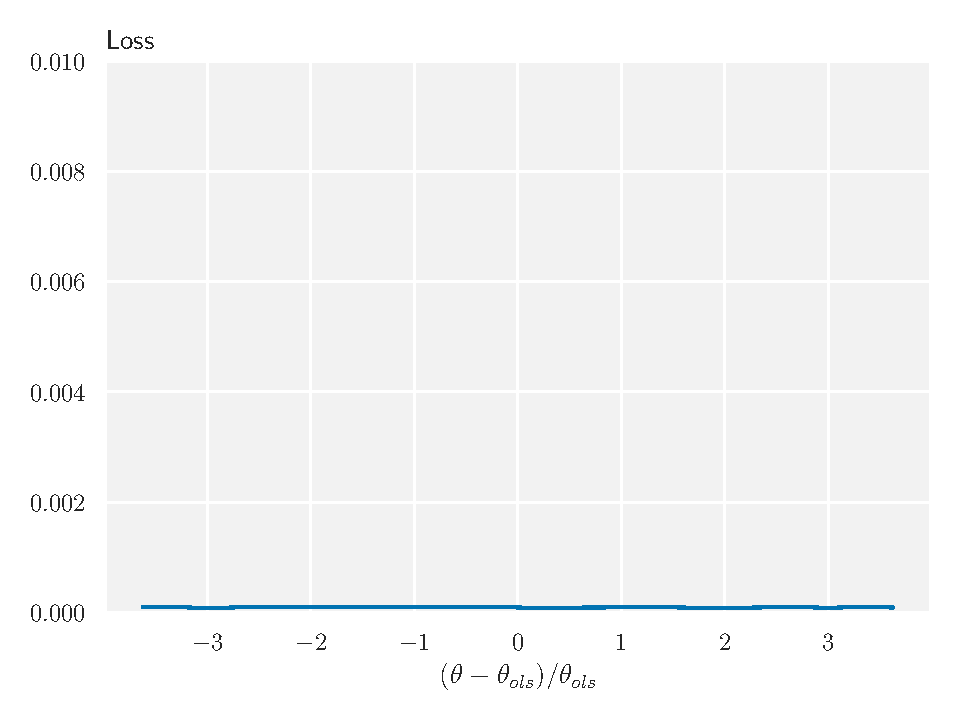
\includegraphics[width=.60\linewidth]{figures/framework/Bazzi_overparam_50000.pdf}
%     %\caption{All zip codes}
%     \label{SUBFIGURE LABEL 3}
% \end{figure}



\begin{align*} 
& \textrm{linearModel} \ \textcolor{blue}{\text{data}} \\
& \textrm{linearModel} \circ \ \textrm{identityMap} \ \textcolor{blue}{\text{data}} \\ 
& \textrm{linearModel} \circ  \big(\textrm{featureMap} \ \textcolor{blue}{\text{data}}\big) \ \textcolor{purple}{\text{params}} \\ 
& \textrm{linearModel} \circ  \big(\textrm{featureMap} \ \textcolor{blue}{\text{data}}\big) \circ \textrm{identityMap} \  \textcolor{purple}{\text{params}} \\ 
& \textrm{linearModel} \circ  \big(\textrm{featureMap} \ \textcolor{blue}{\text{data}}\big) \circ \big(\textrm{clusterMap} \ \textcolor{blue}{\text{data}}\big)  \textcolor{purple}{\text{params}} \\ 
& \textrm{linearModel} >=>  \big(\textrm{featureMap} \ \textcolor{blue}{\text{data}}\big) >=> \big(\textrm{clusterMap} \ \textcolor{blue}{\text{data}}\big)  \textcolor{purple}{\text{params}} \\ 
\end{align*}
While our framework is introduced and well-motivated in a cross-sectional setting with clustered treatment assignment, we apply it in this paper in a repeated cross-section setting. The advantage of our approach in this context, in contrast to a more traditional non-parametric difference-in-difference estimator, is that we explicitly correct for the presence of clustered data in a nonparametric way using pre and post-treatment information. If we let $Z_i, X_i, A$ denote zip code, covariates, and the set of treated clusters respectively, then in a cross sectional setting, our approach allows us to estimate the following conditional expectation functions. 
\begin{align*}
    E[Y_i |X_i, C_i \in A], \qaud    E[Y_i |X_i, C_i \in A^c]
\end{align*}
Given this function, it is straightforward to write down sufficient conditions for identification in a repeated cross-sectional setting following \cite{angrist2009mostly} without introducing any functional form assumptions. \par 

The remainer of the paper is organized as follows. Section 2 describes the essential institutional background of the Right to Counsel and Rapid Rehousing. Section 3 introduces the empirical framework. Section 4 sketches out a toy model, clarifying the estimand of interest in this context. Section 5 contains results and further details of the empirical framework as it relates to the repeated cross-sectional setting. Section 6 concludes.   




% \begin{align*}
%     Y_{i,t} = \alpha + \sum _c \gamma_c C_{i} +  \beta_0 \textrm{Post}_i \times \textrm{Treated}_i + \beta_1  \textrm{Post}_i + \beta_2X_{i,t} + \varepsilon_{i,t}
% \end{align*}






%To some extent, this hope has been empirically justified when considering the direct outcomes of eviction cases. Both in the context of small scale randomized control trials as well as in city-wide roll-outs, researchers have generally found positive results with \cite{seron2001impact}  writing that ``Represented tenants are much less likely to have a final judgment and order of eviction against them'' and \cite{cassidy2022effects} reporting that ``Tenants with lawyers are considerably less likely to be subject to possessory judgments.''\footnote{\cite{greiner2012limits} examines the outcomes of two small scale, Massachusetts based, randomized control trials and finds a measurable impact of legal representation in only one of the trials.} \par 

%The concern, though, is that the indirect effects of the policy might diminish or possibly outweigh these positive legal outcomes. Specifically, the concern is that landlords might respond to the policy by making it harder for low-income households to find housing in the first place. As \cite{gunn1995eviction} writes, ``By increasing landlords' costs of doing business, legal services attorneys may enrich their clients at the expense of all other similarly situated poor tenants." And indeed the increase in costs is one of the most consistent findings across the literature as legal services have been shown to increase the duration of eviction proceedings.\footnote{For example, in reference to the duration of eviction proceedings in New York City,  \cite{cassidy2022effects} writes that: ``The number of days between a case filing and a judgment is also significantly longer in the UA zip codes after program implementation.''} The open policy question, then, is the extent to which landlords pass on these perceived costs, and whether these costs are shifted to those who are least able to bear them.\footnote{A lawyer who specializes in evictions wrote via email that `The thing to remember is that higher costs for landlords always get passed on to the tenants in some form (higher rent, deposits, fees, etc.), or the property gets sold, thereby reducing inventory and resulting in higher rents.''} Up to this point, there has been little to no empirical work on this question. \par 








 


\section{Background \& Policy Details}
\subsection{Evictions}
\begin{itemize}
    \item Grace Period
    \item Serve notice to quit
    \item Summons \& Complaints 
    \item Judgement \& Resitution (Control of property is returned to the landlord 
\end{itemize}

\subsection{Implementation}
Signed in June of 2021 by Governor Lamont, the Right to Counsel went into effect on January 31, 2022, as rental relief services in response to Covid-19 we're coming to an end, well after the expiration of the CDC's eviction moratorium for nonpayment of rent (August 26, 2021). Because the expected demand for legal services under the Right to Counsel exceed the level of legal support, state representatives rolled out the policy in phases.  In the first stage, the policy was made available to a subset of the zip codes (the 14 shown in yellow) in figure \ref{fig:treated_areas} which make up $30\%$ of evictions and $20\%$ percent of the renter population (Connecticut Bar Foundation). The expectation was that 2,000 households would receive legal aid in the first phase out of the 20,000 households expected. Individuals and families within these zip codes who made $80\%$ or less than the area median income were eligible (\href{https://www.cga.ct.gov/2021/ACT/PA/PDF/2021PA-00034-R00HB-06531-PA.PDF}{Reference}).
\par 
\begin{figure}[htbp]
\centering
    \centering
    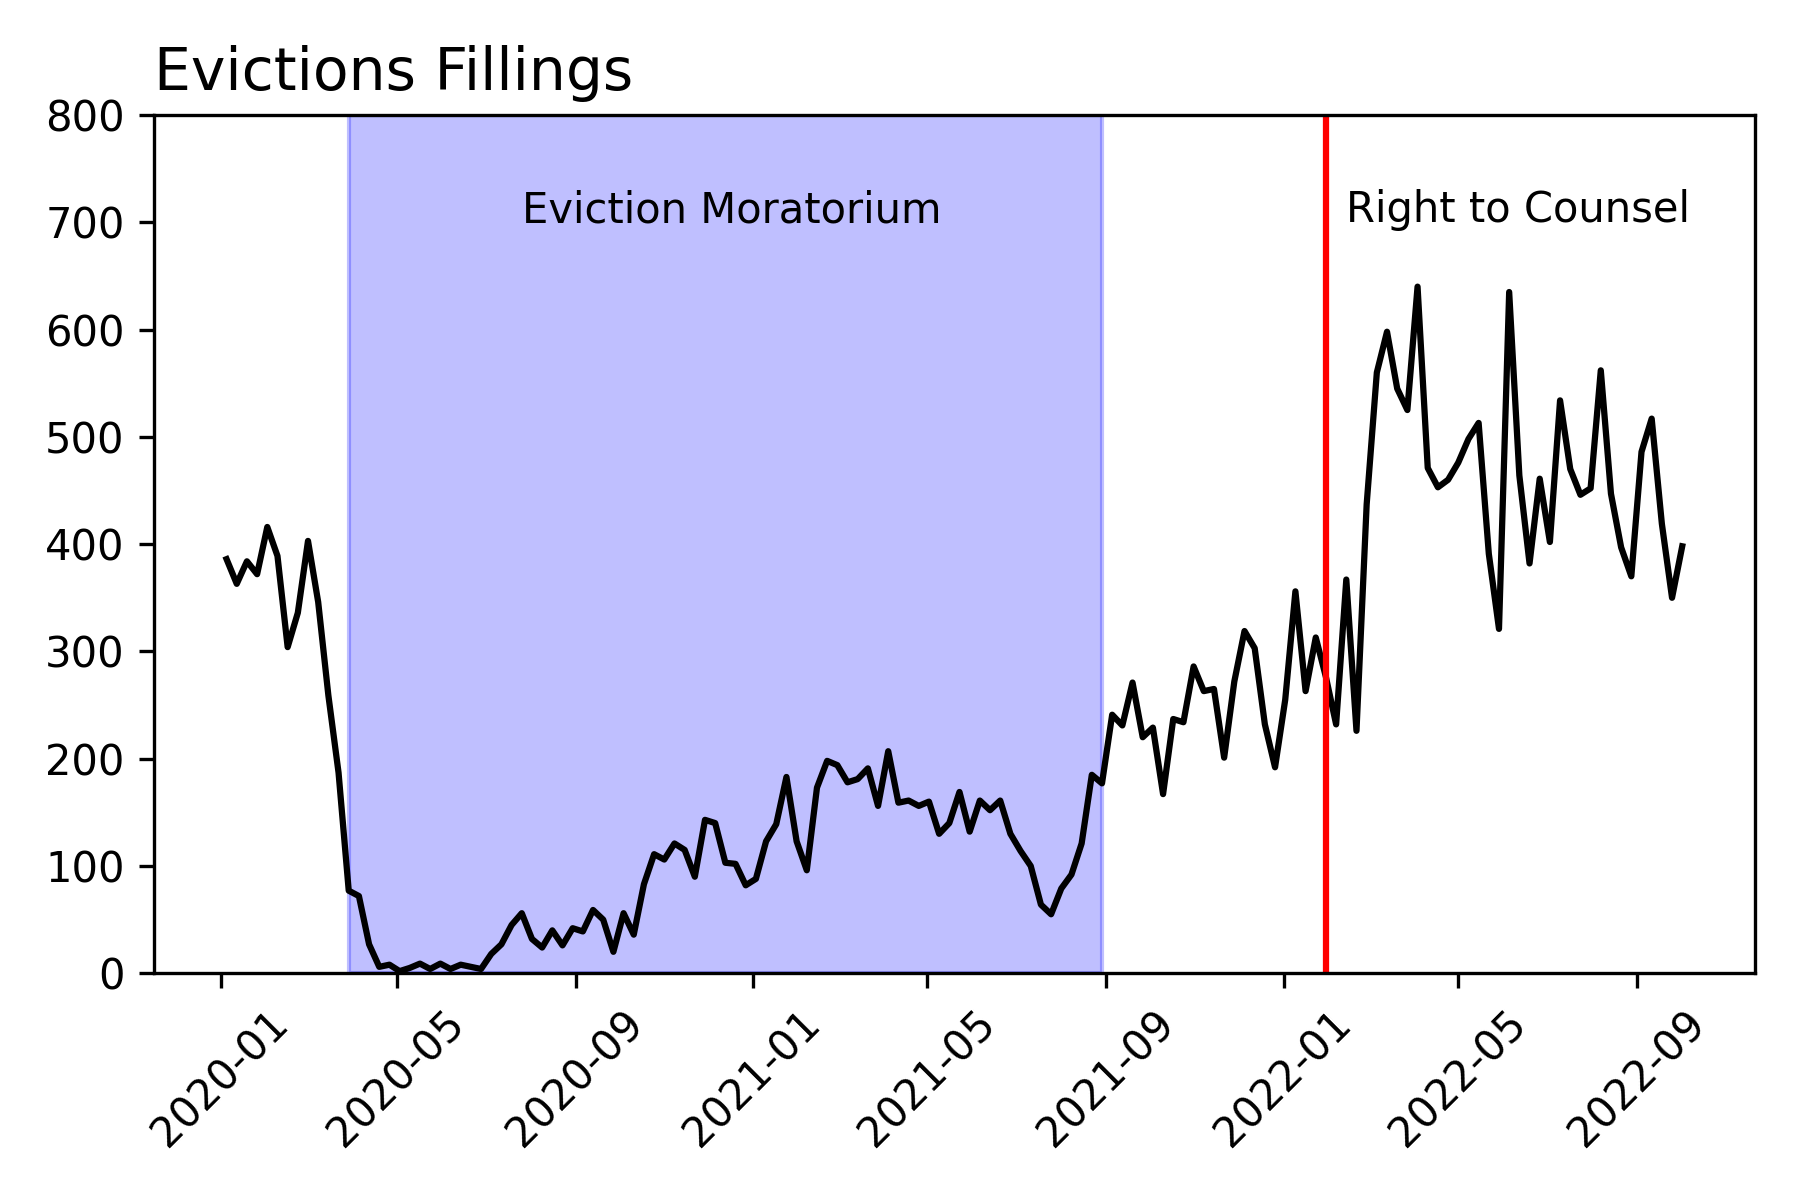
\includegraphics[width=.60\linewidth]{figures/rtc/context/evictions_conn.png}
    \caption{Weekly eviction fillings within the state of Connecticut as reported by the \href{https://evictionlab.org/}{Eviction Lab at Princeton}}
    \label{SUBFIGURE LABEL 3}
\end{figure}
\subsection{Treatment}

\footnote{CBF Assignment Sheet-- received via email on August 26th --}  Beginning earlier, on October 1, 2021, landlords were to notify individuals of the existence of this policy when serving tenants with a notice to quit (the first step in an eviction proceeding -- the entire process is described in more detail in the appendix). In addition to landlords, courts were expected to inform tenants of the policy when and if tenants appeared in court.\footnote{\href{https://www.cga.ct.gov/2021/ACT/PA/PDF/2021PA-00034-R00HB-06531-PA.PDF}{``On} and after October 1, 2021, an owner, lessor, landlord, legal
representative or agent of an owner, lessor or landlord, a housing
authority or a housing subsidy program administrator, as applicable,
shall attach a copy of the notice described under subdivision (1) of this
subsection, to (A) a notice to quit delivered to a covered individual
pursuant to chapter 832 or chapter 412 of the general statutes; (B) a
summons and complaint for a summary process action pursuant to
chapter 832 or chapter 412 of the general statutes; (C) a lease termination
notice for a public or subsidized housing unit; and (D) a notice to
terminate a state or federal housing subsidy''}\footnote{\href{https://www.cga.ct.gov/2021/ACT/PA/PDF/2021PA-00034-R00HB-06531-PA.PDF}{``An}y court notice scheduling a mediation or hearing that is sent to
a self-represented party in a covered matter shall include plain language
information about the availability of legal representation through the
right to counsel program and a phone number for accessing information
and applying for assistance.''} Given that the lack of enforcement with respect to landlords and that $37\%$ of Connecticut tenants fail to appear in court during eviction proceedings, it's quite possible that many eligible tenants are not yet aware of the policy's existence.\footnote{According to \href{https://www.ctpublic.org/news/2022-01-30/some-residents-facing-eviction-could-now-be-eligible-for-free-legal-aid}{article} $37\%$ of Connecticut tenants fail to appear in court during eviction proceedings, and their cases end in default, according to a 2021 report by the Connecticut Advisory Council on Housing Matters.}

\begin{figure}[htbp]
\centering
\begin{subfigure}{.48\textwidth}
    \centering
    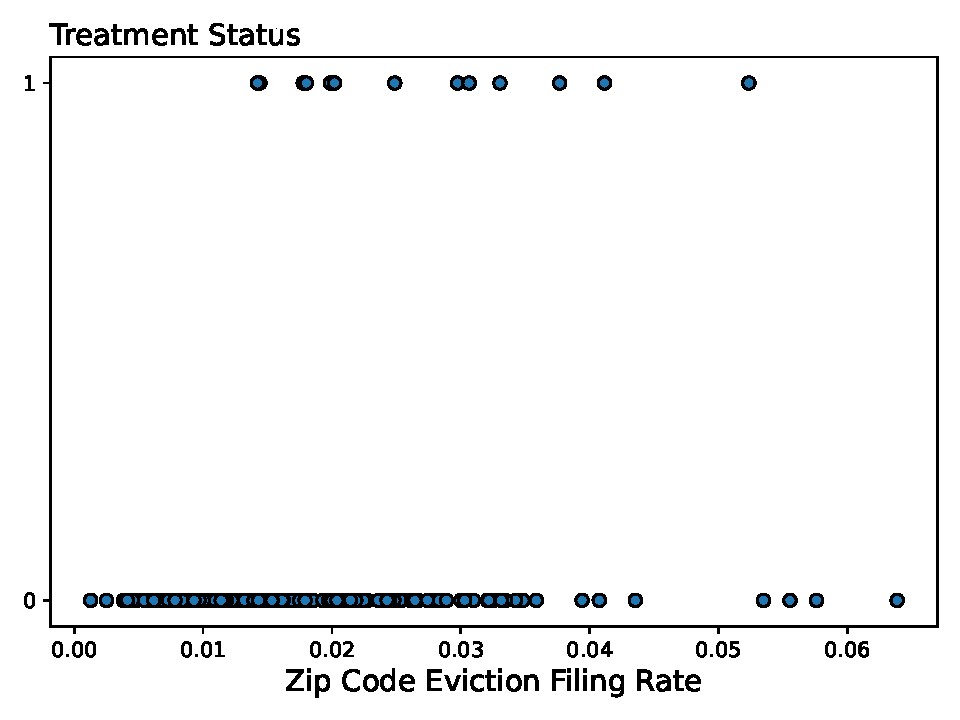
\includegraphics[width=.95\linewidth]{figures/rtc/context/eviction_filing_rate_per_pop.pdf}
    \caption{Eviction Filing Rates}
    \label{fig:efr}
\end{subfigure}
\begin{subfigure}{.48\textwidth}
    \centering
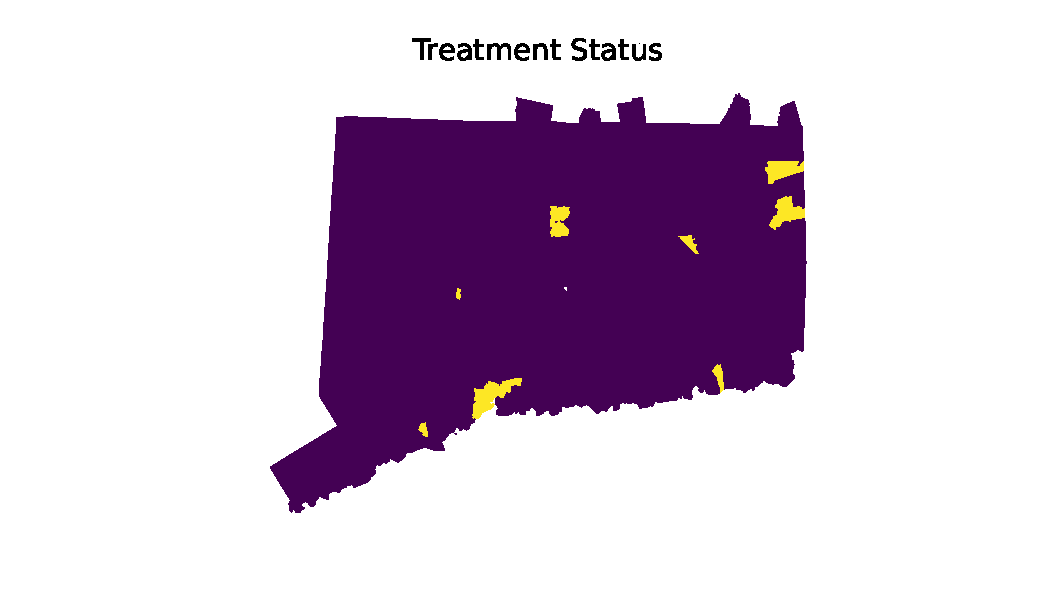
\includegraphics[width=0.95\textwidth]{figures/rtc/maps/zip_code_status.pdf}  
        \caption{Treatment status for each zip code (yellow indicates treated zip code): \href{https://github.com/pharringtonp19/evictions/blob/main/scripts/joint/maps/treatment_status.py}{Reproduced Here}}
    \label{fig:treated_areas}
\end{subfigure}
\caption{The general pattern that these figures try to highlight is that in order to fit the the `v`-shaped valley in the function, the model overfits the tails of the function -- \href{https://github.com/pharringtonp19/jmp_paper/blob/main/notebooks/gradient_descent_motivating_example.ipynb}{Reproduced Here}}
%\label{FIGURE LABEL}
\end{figure}

\subsection{Data \& Outcomes}
As referenced prior, the outcome of interest is the search length for households who are currently experiencing homelessness but face limited barriers to housing. Rapid Re-housing, a federally tracked program, provides limited short term assistance to exactly this population.\footnote{As \cite{evans2019reducing} explains, ``The
Homeless Management Information System (HMIS) is a nationwide network of local IT systems that collect
client-level data for people entering sheltered services. These systems are organized at the CoC level and most
homeless shelters across the country are part of the HMIS system''} Its aim is to help ``families exit shelters and get back into permanent housing quickly.''\footnote{\textrm{Missing Source}} While different in nature than an independent housing search, the search length of individuals in a Rapid Rehousing program a reasonable proxy for the following three reasons. First, Rapid Rehousing programs ``serve people experiencing homelessness with no preconditions such as employment, income, absence of criminal record, or sobriety.''\footnote{\href{https://www.urban.org/sites/default/files/publication/99153/rapid_re-housings_role_in_responding_to_homelessness_3.pdf}{Reference}} Second, the program does not target people who might need long-term assistance. Those individuals and families are helped by permanent supportive housing programs.\footnote{Very different from permanent supportive housing which is as Rosanne Haggerty writes in the NyTimes, ``is ideal for those with serious health challenges who have been homeless for long periods of time''.\footnote{\href{https://www.nytimes.com/roomfordebate/2015/02/19/homes-for-the-homeless/for-even-the-neediest-housing-is-the-solution-to-homelessness}{NyTimes}}}\footnote{ \textbf{Cost}: at $\$6,678$ per family, it is cheaper than transitional housing at $\$32,557$ per family.\footnote{\href{https://cceh.org/provider-resources/rapid-rehousing/}{CCEH Video}}} Third, the lease agreement households sign come with ``the same rights and responsibilities as a typical lease holder.''\footnote{\href{thttps://endhomelessness.org/resource/rapid-re-housing-a-history-and-core-components/}{It} is imperative that any lease agreement provides the tenant with **the same rights and responsibilities as a typical lease holder** and that the financial terms of the lease are such that the household has a reasonable ability to assume rental costs once financial support ends (keeping in mind that in the majority of cases, even households with no income at move-in retain their housing)"}
\begin{itemize}
    \item \cite{evans2019reducing}: The Family Options Study provides the primary experimental test of the effectiveness of rapid rehousing (RRH), but the results for this treatment arm are mixed. There were no statistically significant
differences in housing outcomes between the control and short-term subsidy group by the three-year followup. (Gubits et al. 2016).
\end{itemize}
\begin{figure}[htbp]
\centering
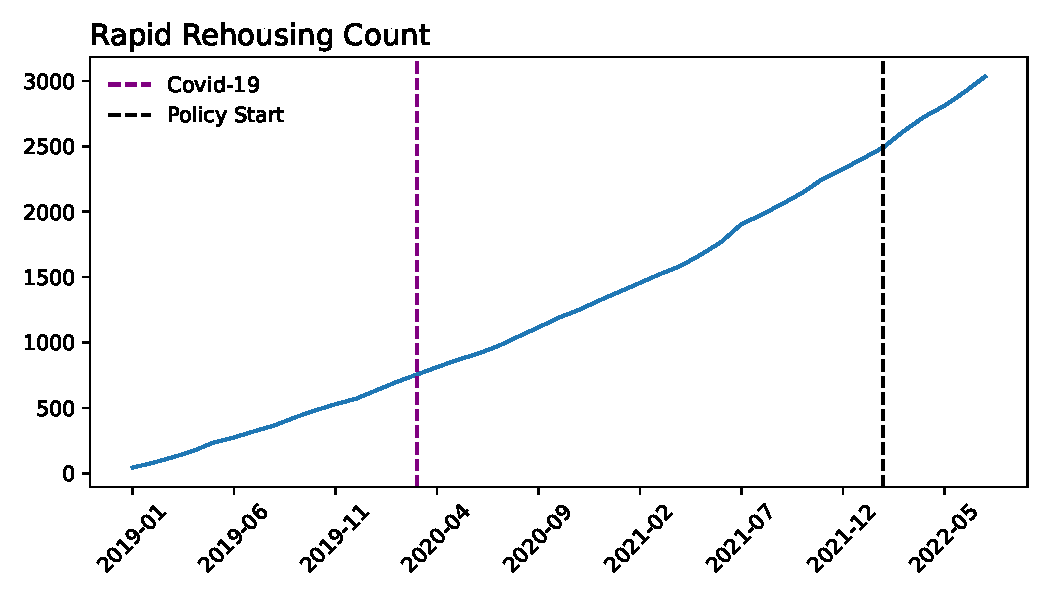
\includegraphics[width=0.7\textwidth]{figures/rtc/context/rrh_counts.pdf}
        \caption{Treatment status for each zip code (yellow indicates treated zip code): \href{https://github.com/pharringtonp19/evictions/blob/main/scripts/cceh/plot/summary_rrh.py}{Reproduced Here}}
\end{figure}
\section{Framework}
\label{sec:framework}
\subsection{Context}
To keep things simple, we describe our approach in the specific context of cluster-level randomized control trials where we're interested in estimating treatment heterogeneity. Cluster-level randomized control trials are randomized control trials where treatment varies at a level above the unit of interest. Such experiments are common in development, education, and health settings because they are (A) generally easier to implement (\cite{gerber2012field}), (B) better adhere to the potential outcome framework (\cite{imbens2015causal}) and perhaps most importantly (C) allow us to understand the the effects of scaling the treatment (\cite{list2021voltage}). 


\subsection{Challenge (\textcolor{blue}{The Tragic Triad})\footnote{The expression ``tragic triad" is taken from \cite{yu2020gradient}}}
In the absence of cluster data, under the selection on observable and stable unit treatment value assumptions, such an estimation problem is equivalent to solving the following optimization problem over the treatment and controls groups separately. 

\begin{align*}
    \underset{f \in \sigma(X)}{\textrm{inf}} \ \mathbb{E}\big[(Y-f )^2\big] 
\end{align*}
 
Under the potential outcome framework, clustered level treatment assignment poses a few challenges because in each group: (1) we observe only a subset of the clusters, (2) the distribution of covariates can differ across clusters, and (3) the distribution of outcomes conditional on covariates may differ across clusters. These issues are perhaps only magnified as we increase the dimensionality of the data. As shown in figure \ref{fig:high}, we extended the work of \cite{balestriero2021learning} to the situation of clustered sampling. As illustrated in figure \ref{fig:higha}, clustered sampling doesn't change the fundamental issue of learning in high dimensions  (extrapolation) so much as it motivates us to reconsider how we go about it, as highlighted in figure \ref{fig:highb}.
\begin{figure}[htbp]
\centering
\begin{subfigure}{.48\textwidth}
    \centering
    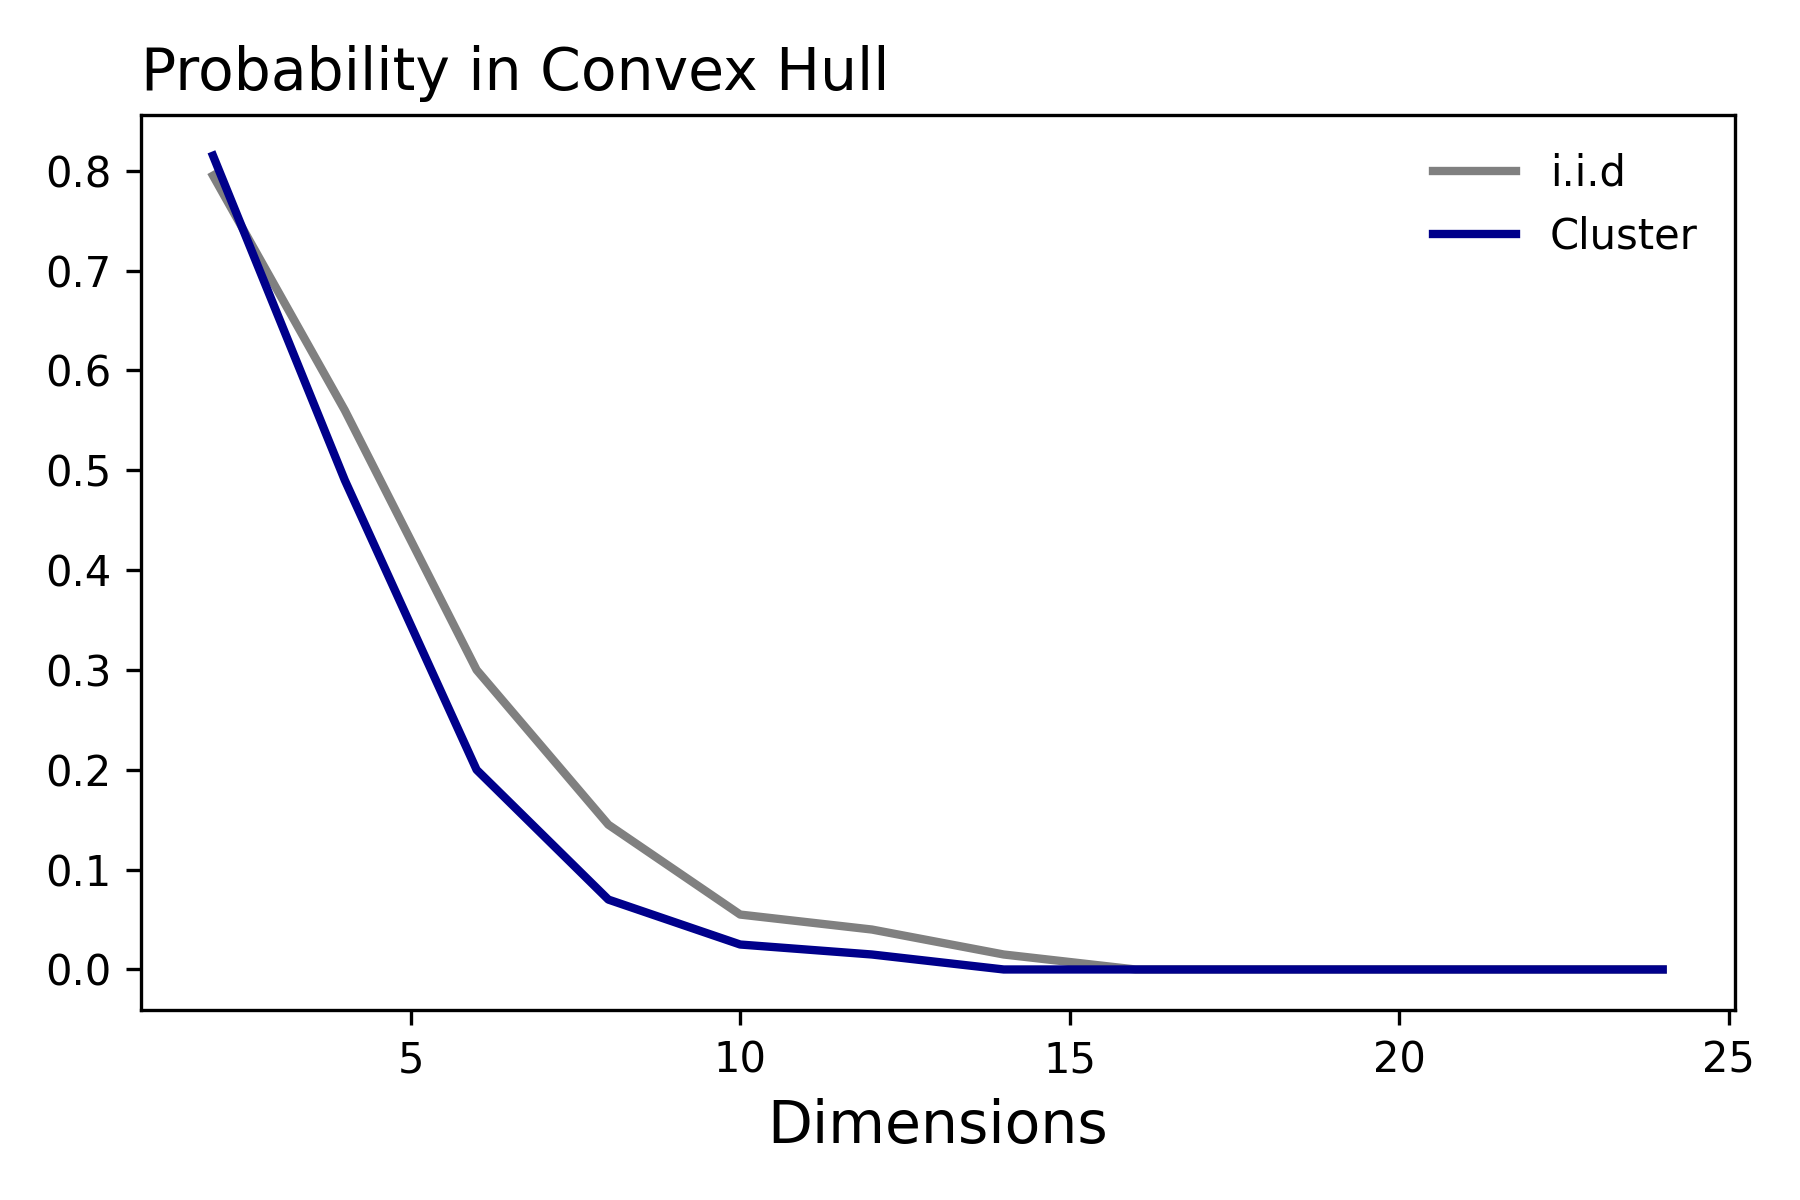
\includegraphics[width=.95\linewidth]{figures/framework/iid_cluster.png}
    \caption{}
    \label{fig:higha}
\end{subfigure}
\begin{subfigure}{.48\textwidth}
    \centering
    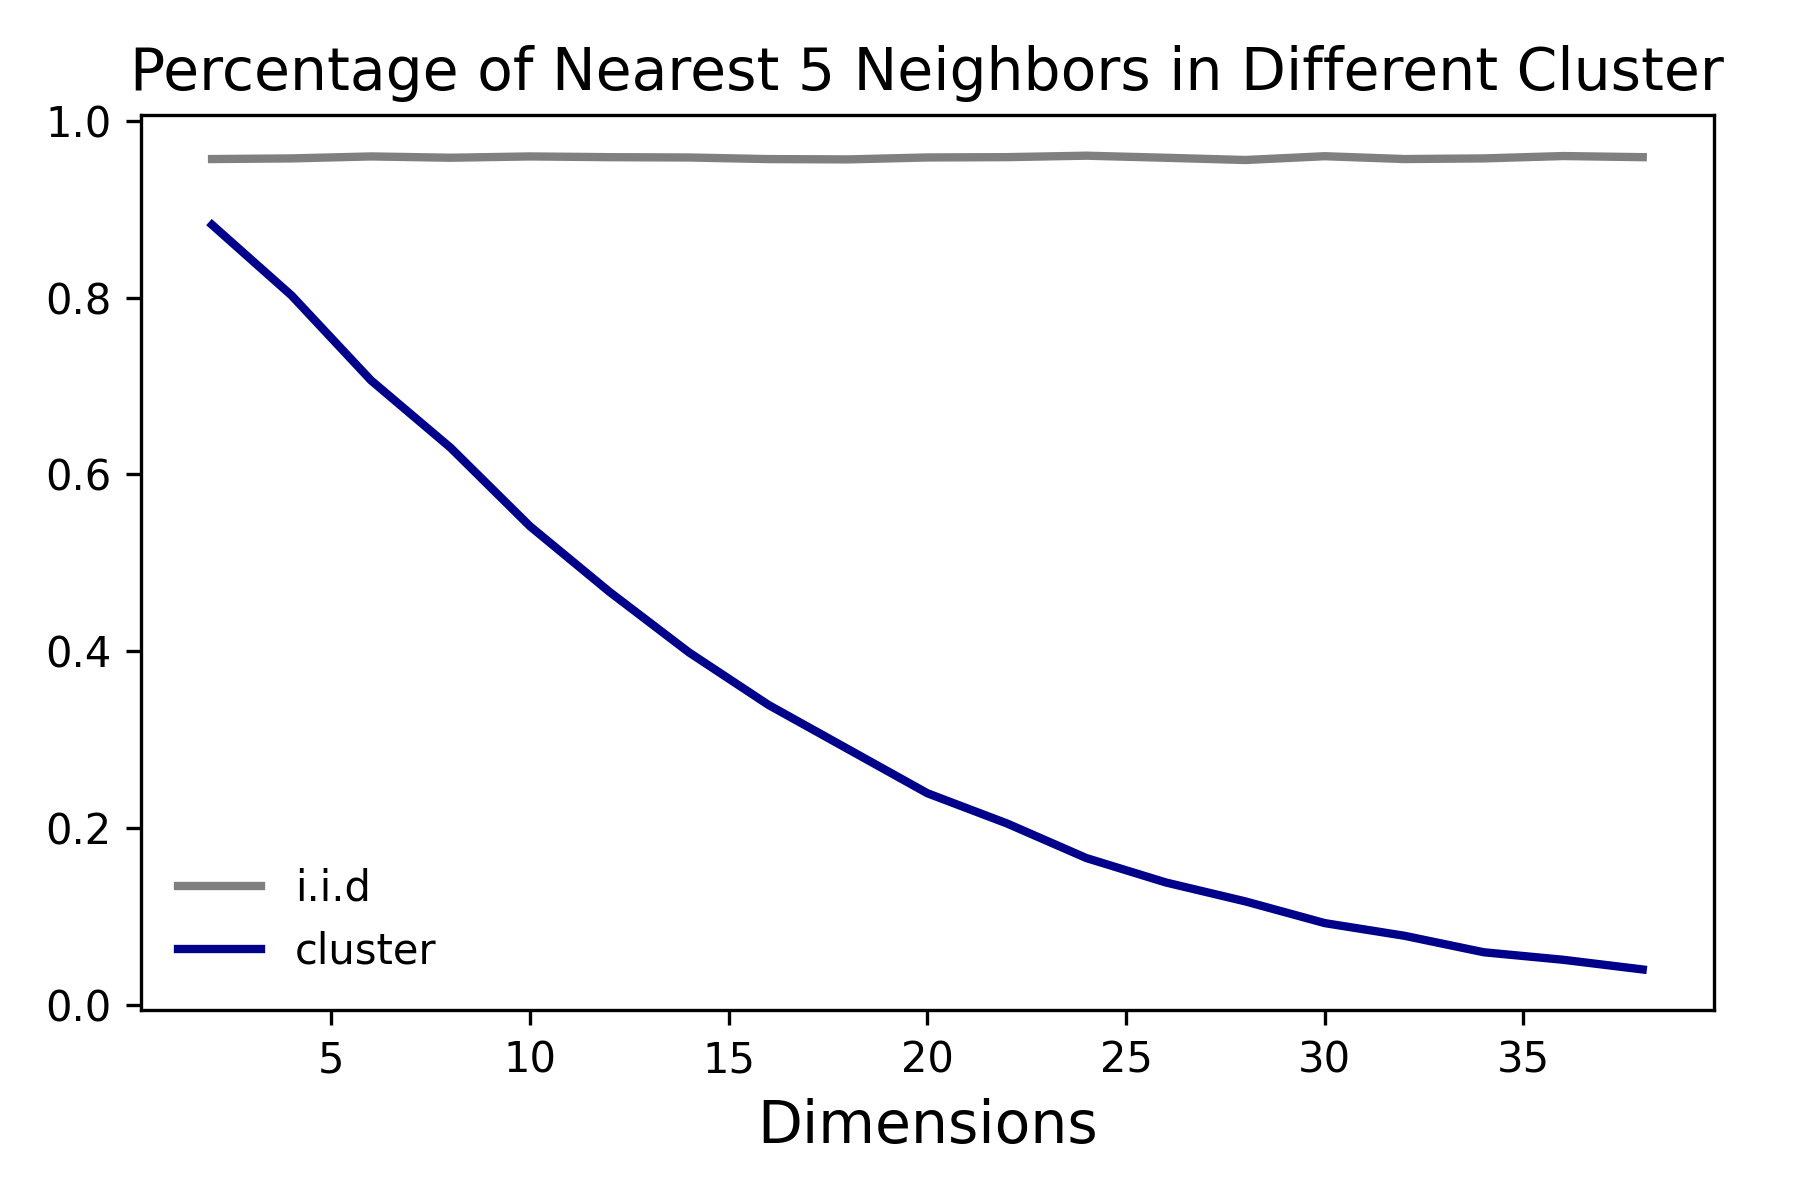
\includegraphics[width=.95\linewidth]{figures/framework/nearest_neighbors_increasing_correlation.png}
    \caption{}
    \label{fig:highb}
\end{subfigure}
\caption{(a) Probability that a observation in the test set is in the convex hull formed by the training set (b)  Fraction of the five nearest neighbors in a different cluster. Data consists of 25 cluster and 25 observations per cluster. Clusters differ only in the mean which is drawn from multivariate normal distribution with an identity covariance matrix: Reproduced \href{https://github.com/pharringtonp19/rfp/blob/main/notebooks/How_Input_Normalization_Changes_Our_Understanding_of_Interpolation_vs_Extrapolation_With_Clusters.ipynb}{Here} and  \href{https://github.com/pharringtonp19/rfp/blob/main/notebooks/Nearest_Neighbors_Example.ipynb}{Here}}
\label{fig:high}
\end{figure} \par 
We can use the following motivating example to illustrate the pratical challenge. The key issue is how to locally correct for the presence of clustered data. Intuitively, when there are a lot of clusters present, we would prefer a small bandwidth. When there are few clusters present, we would prefer a larger bandwidth. Figure \ref{fig:nonparametrics}
highlights why this local correction is necessary in that in order to fit the the `v`-shaped valley in the function, the model overfits the tails of the function.
\begin{figure}[htbp]
\centering
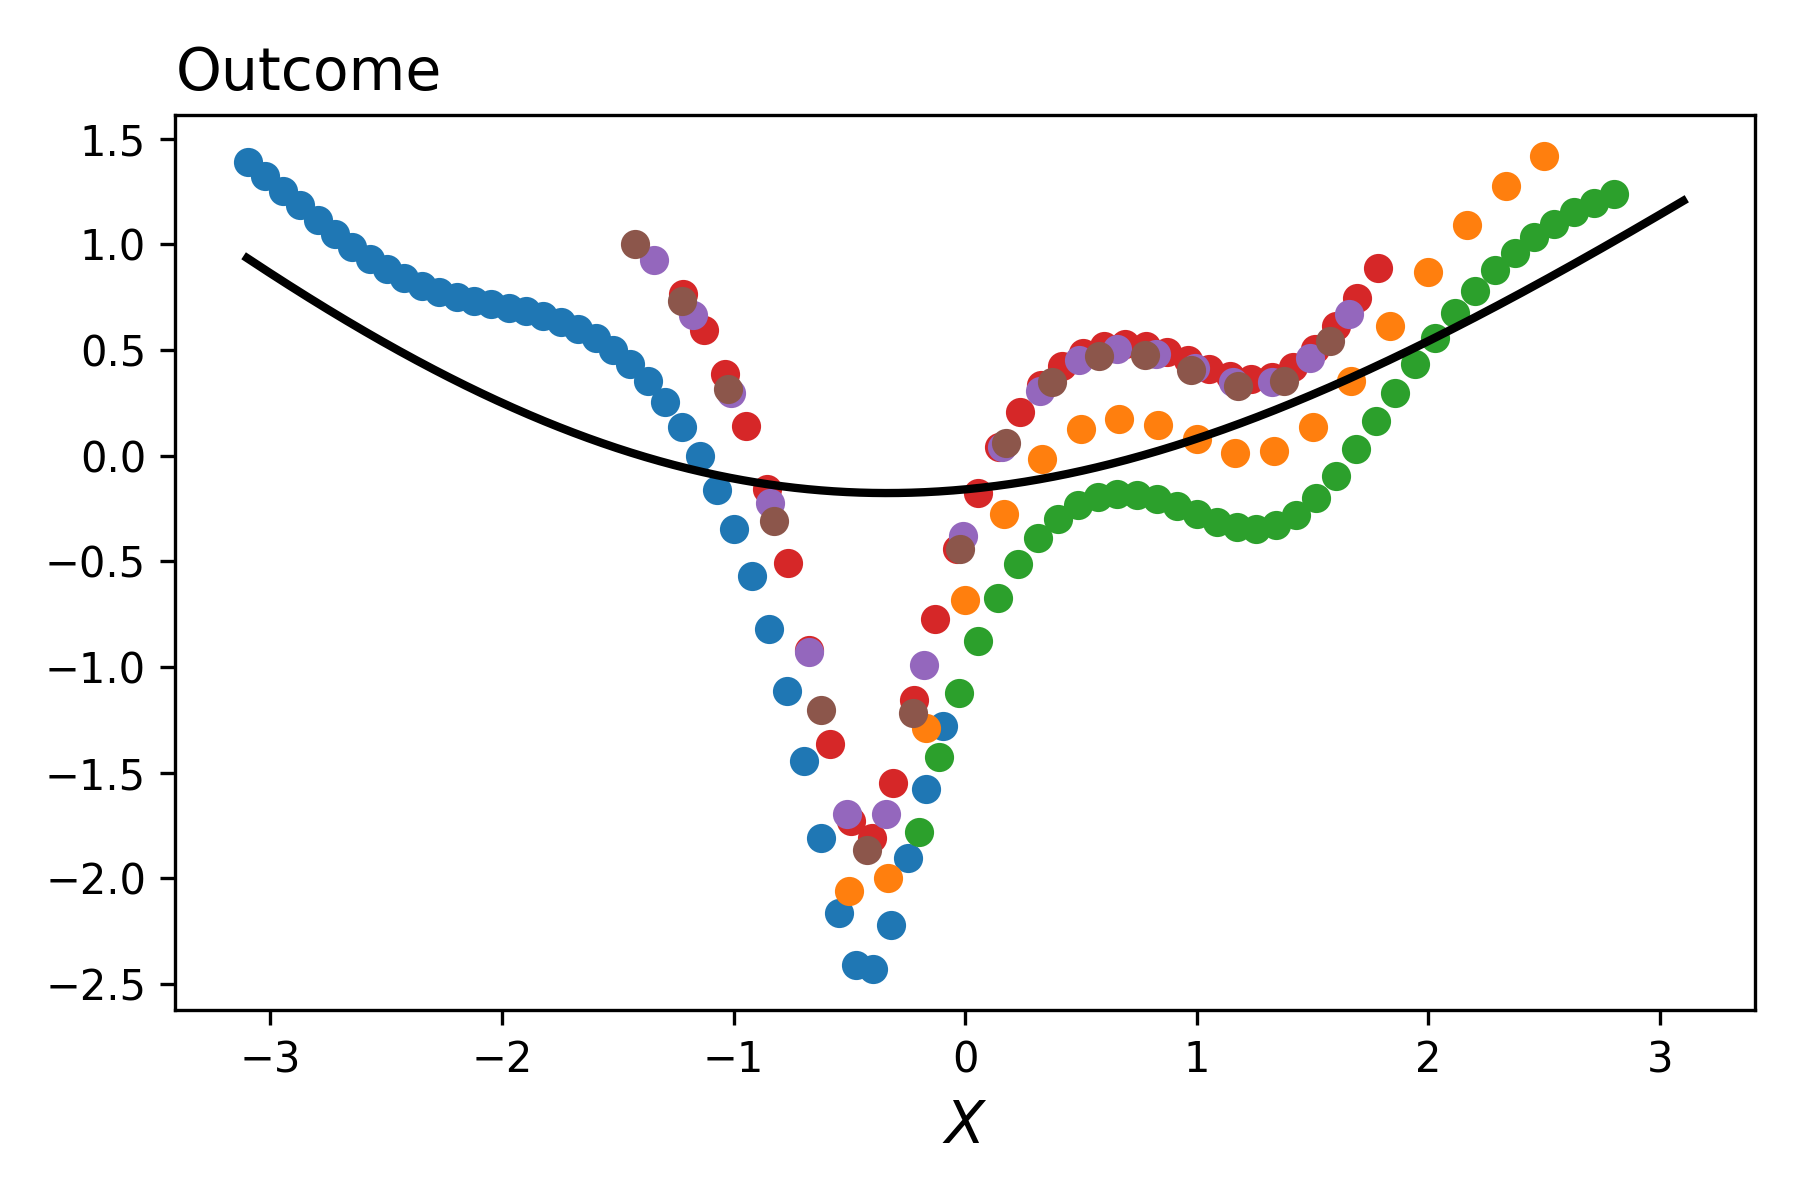
\includegraphics[scale=0.3]{figures/framework/local_linear_no_const_0.5_18_LM.png}
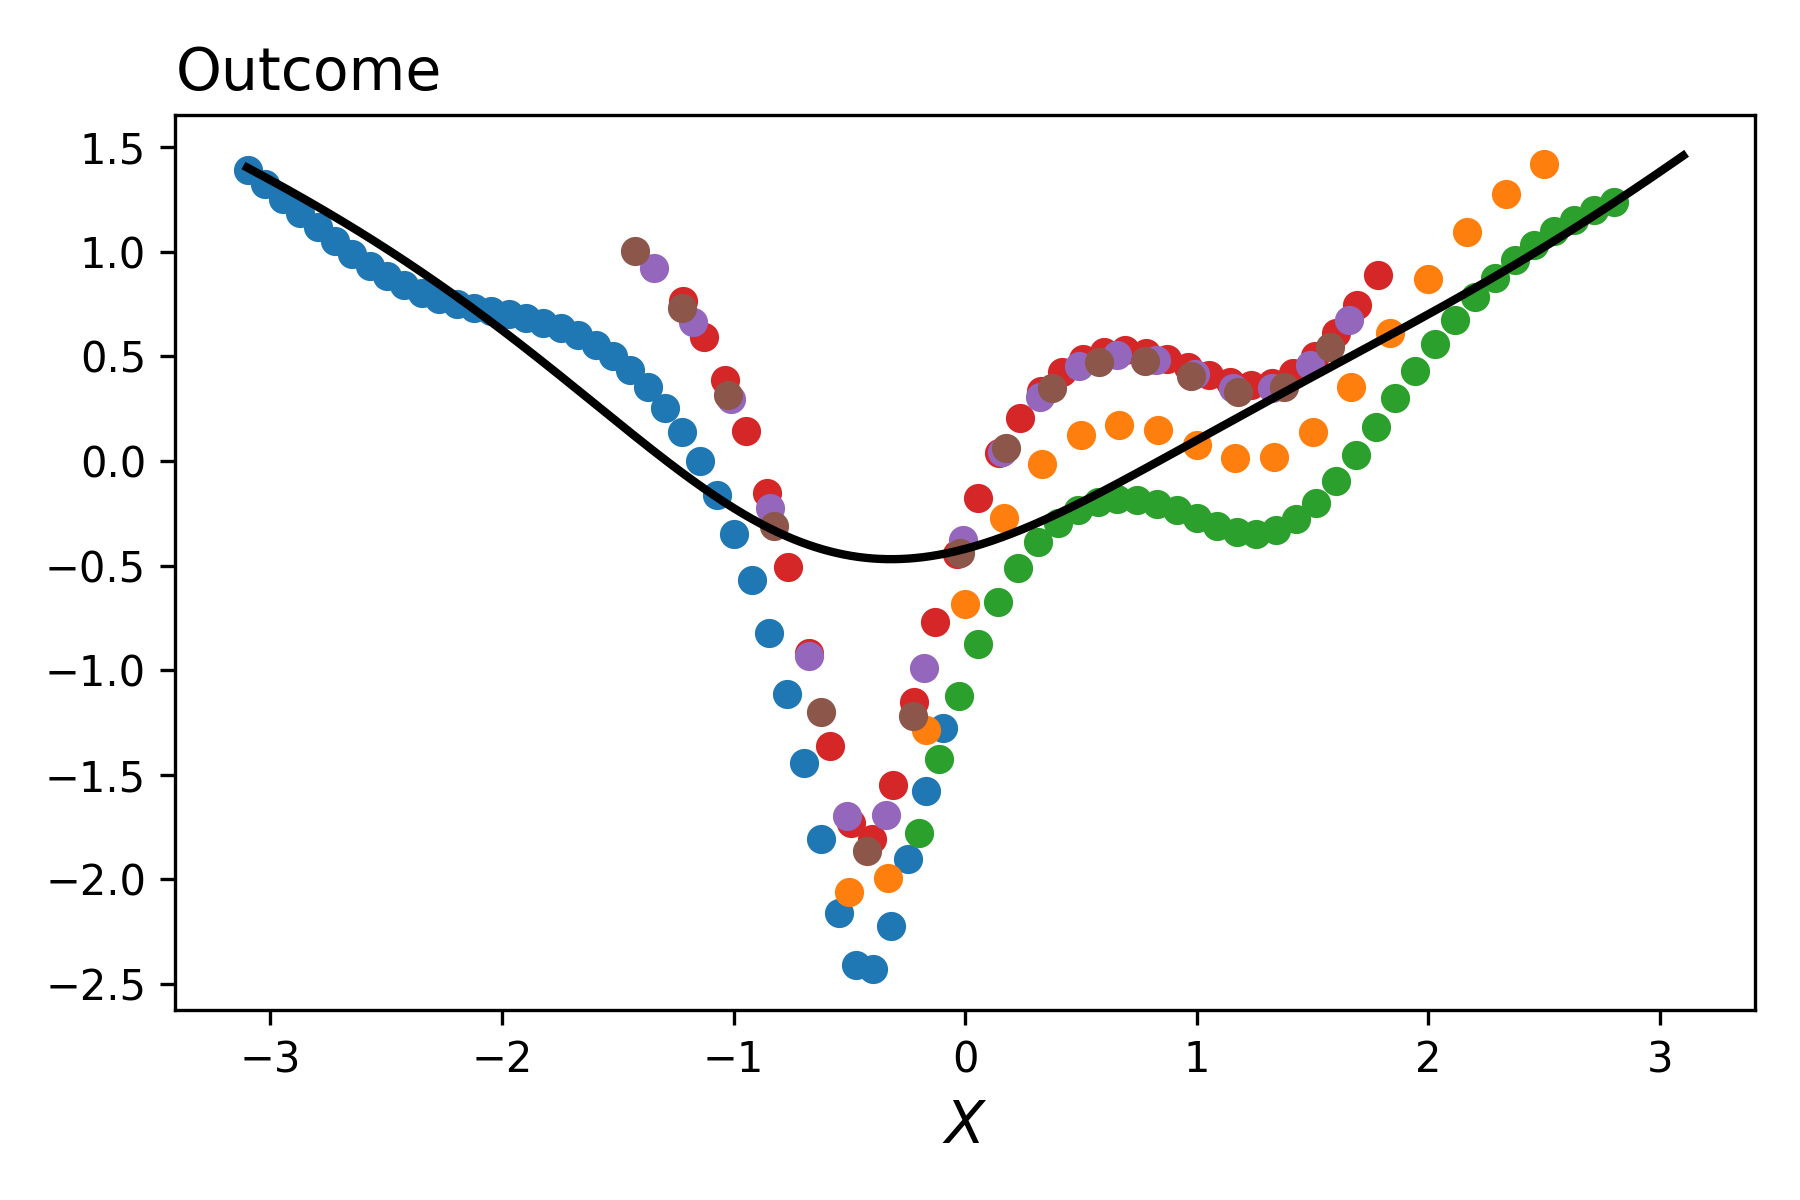
\includegraphics[scale=0.3]{figures/framework/local_linear_no_const_1.0_18_LM.png}
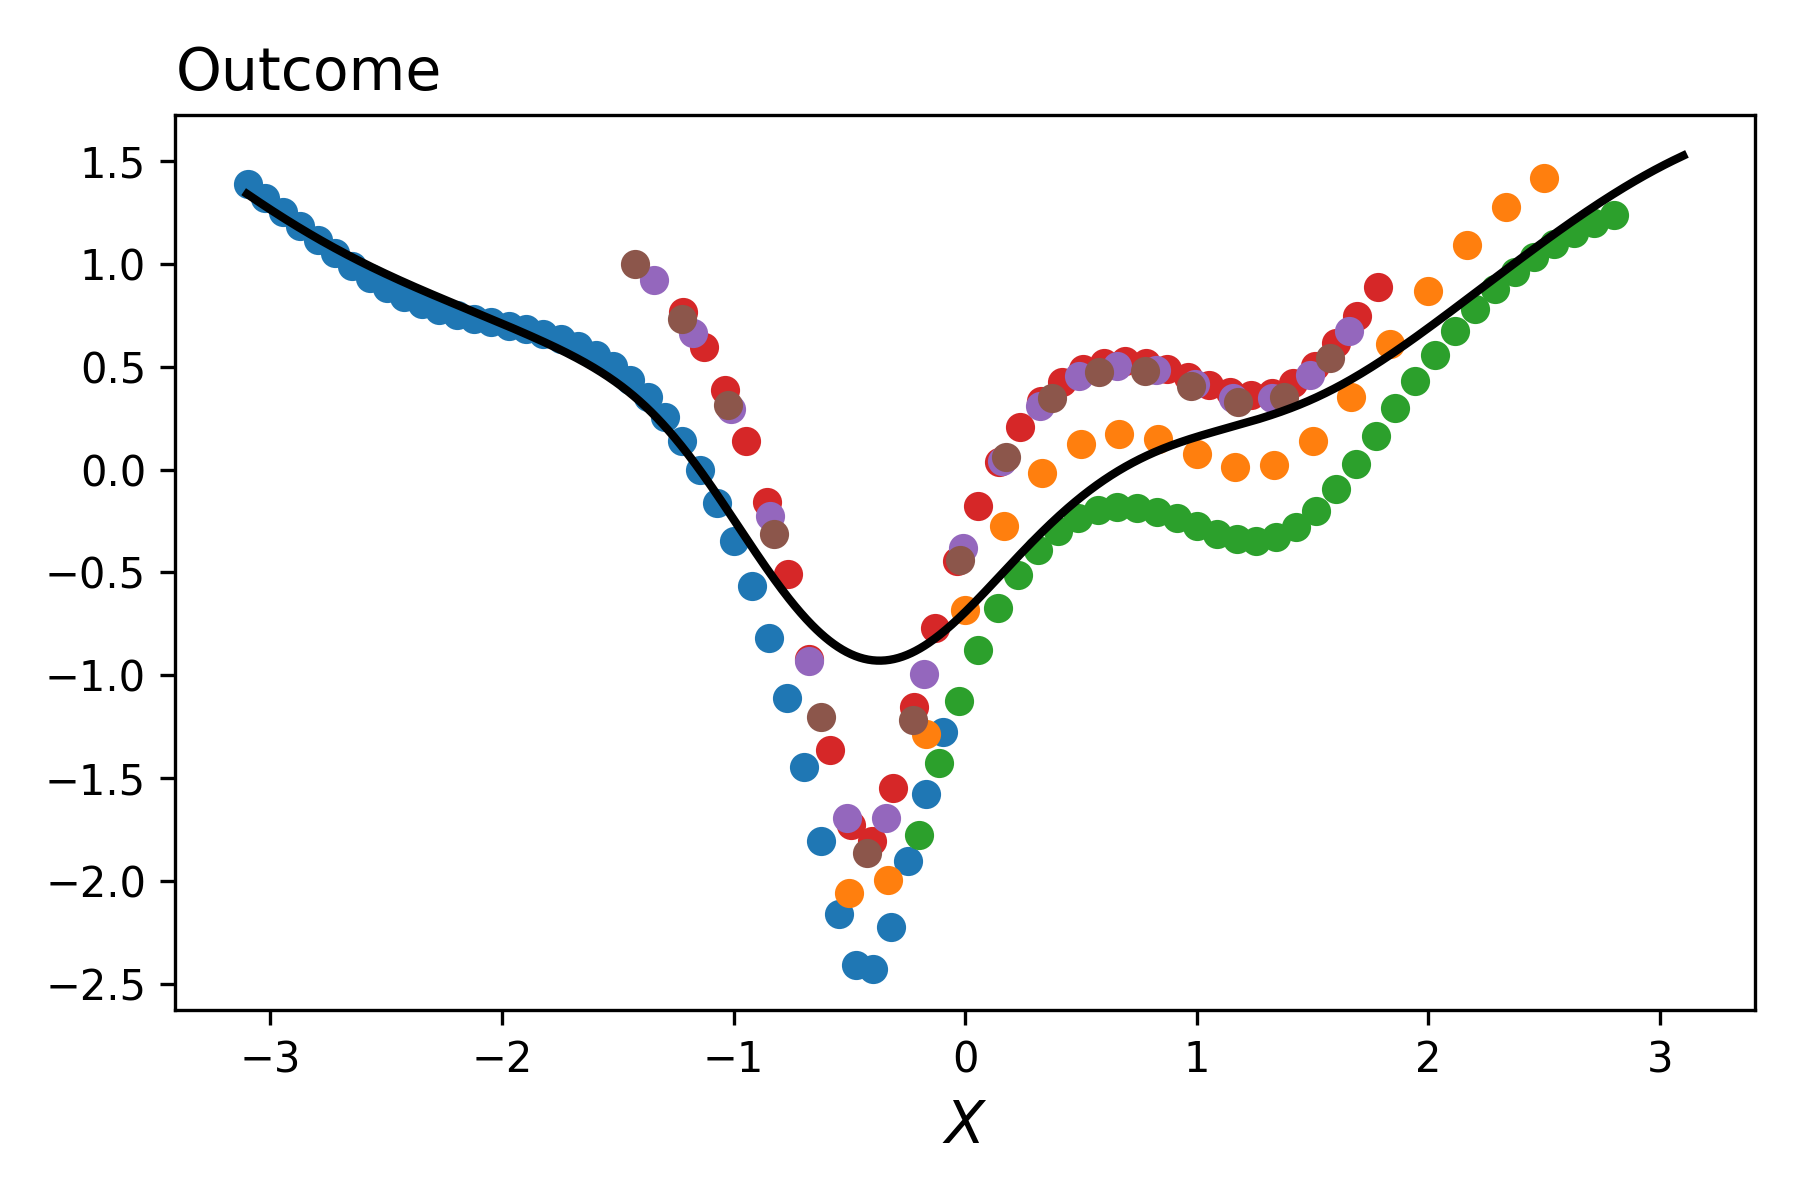
\includegraphics[scale=0.3]{figures/framework/local_linear_no_const_2.0_18_LM.png}
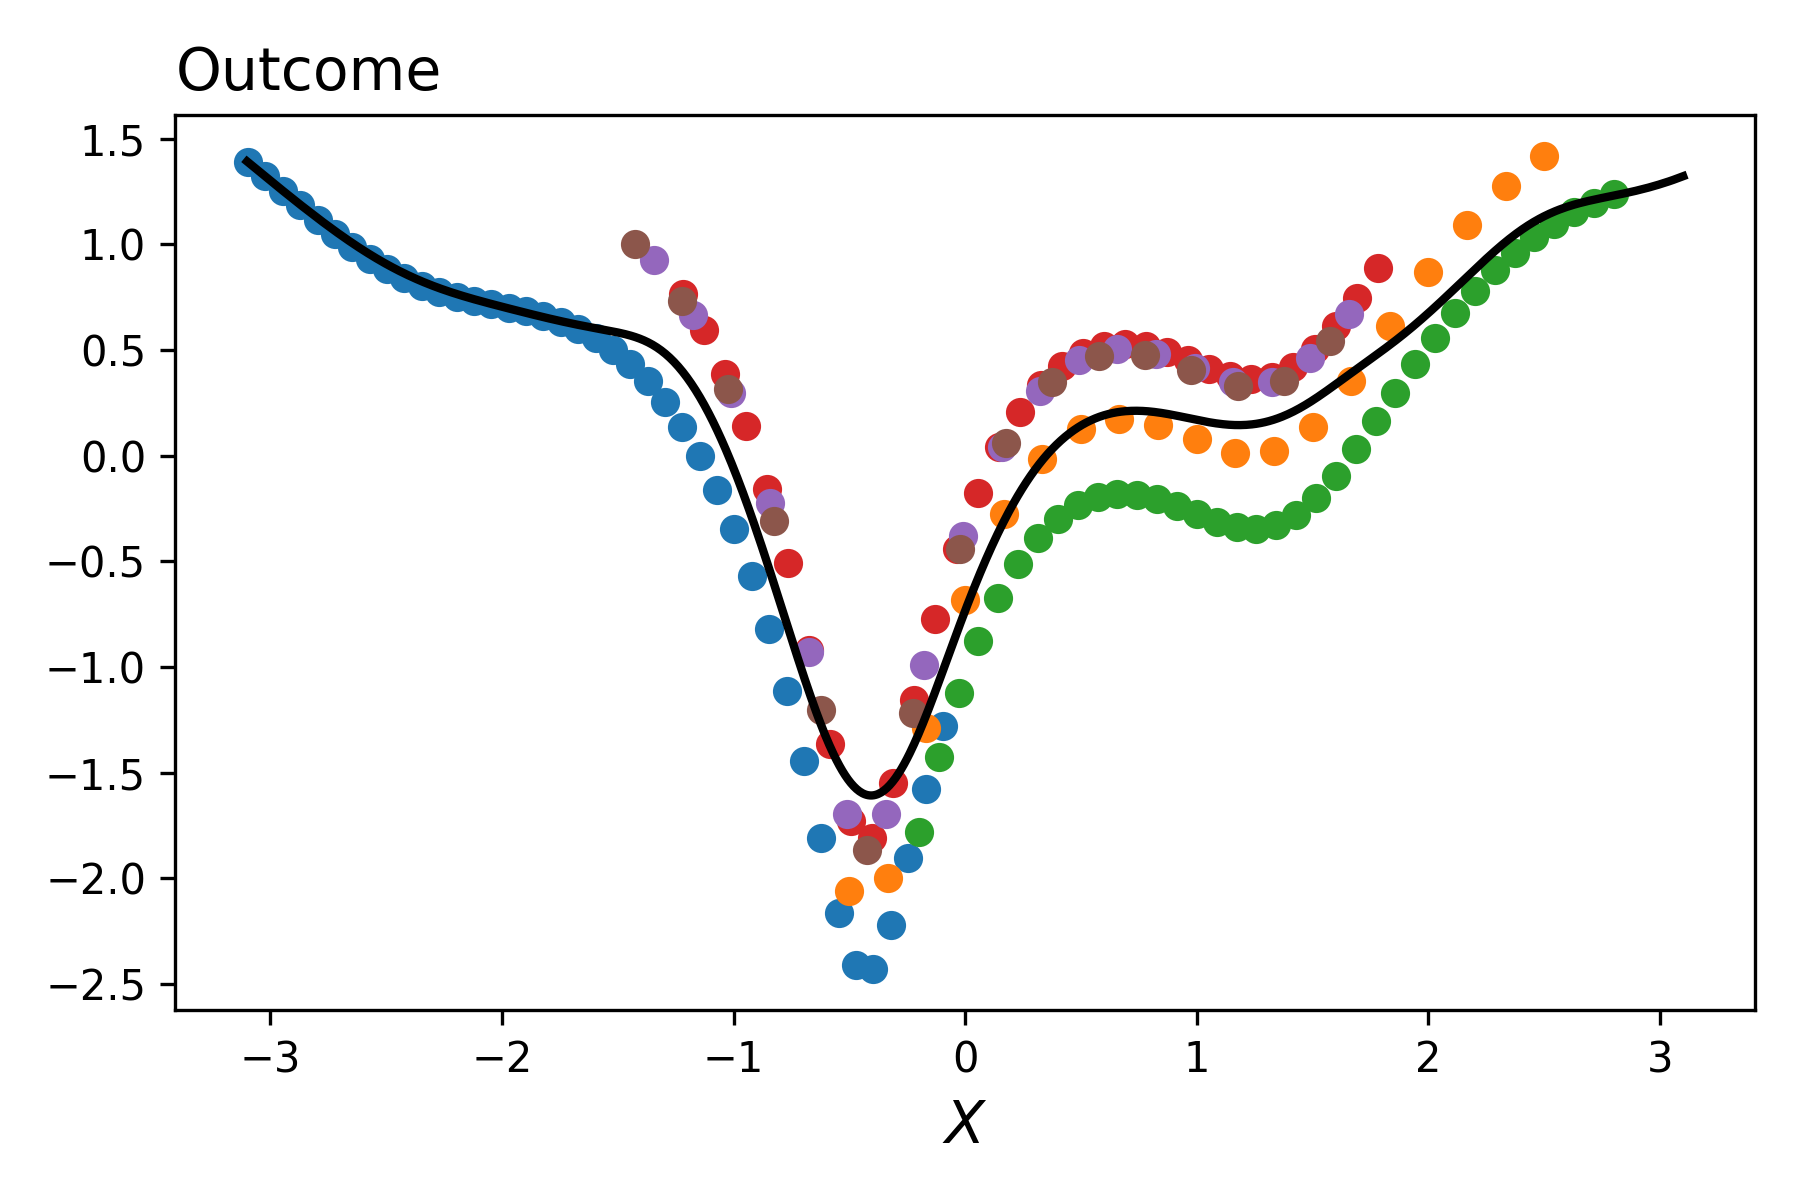
\includegraphics[scale=0.3]{figures/framework/local_linear_no_const_5.0_18_LM.png}
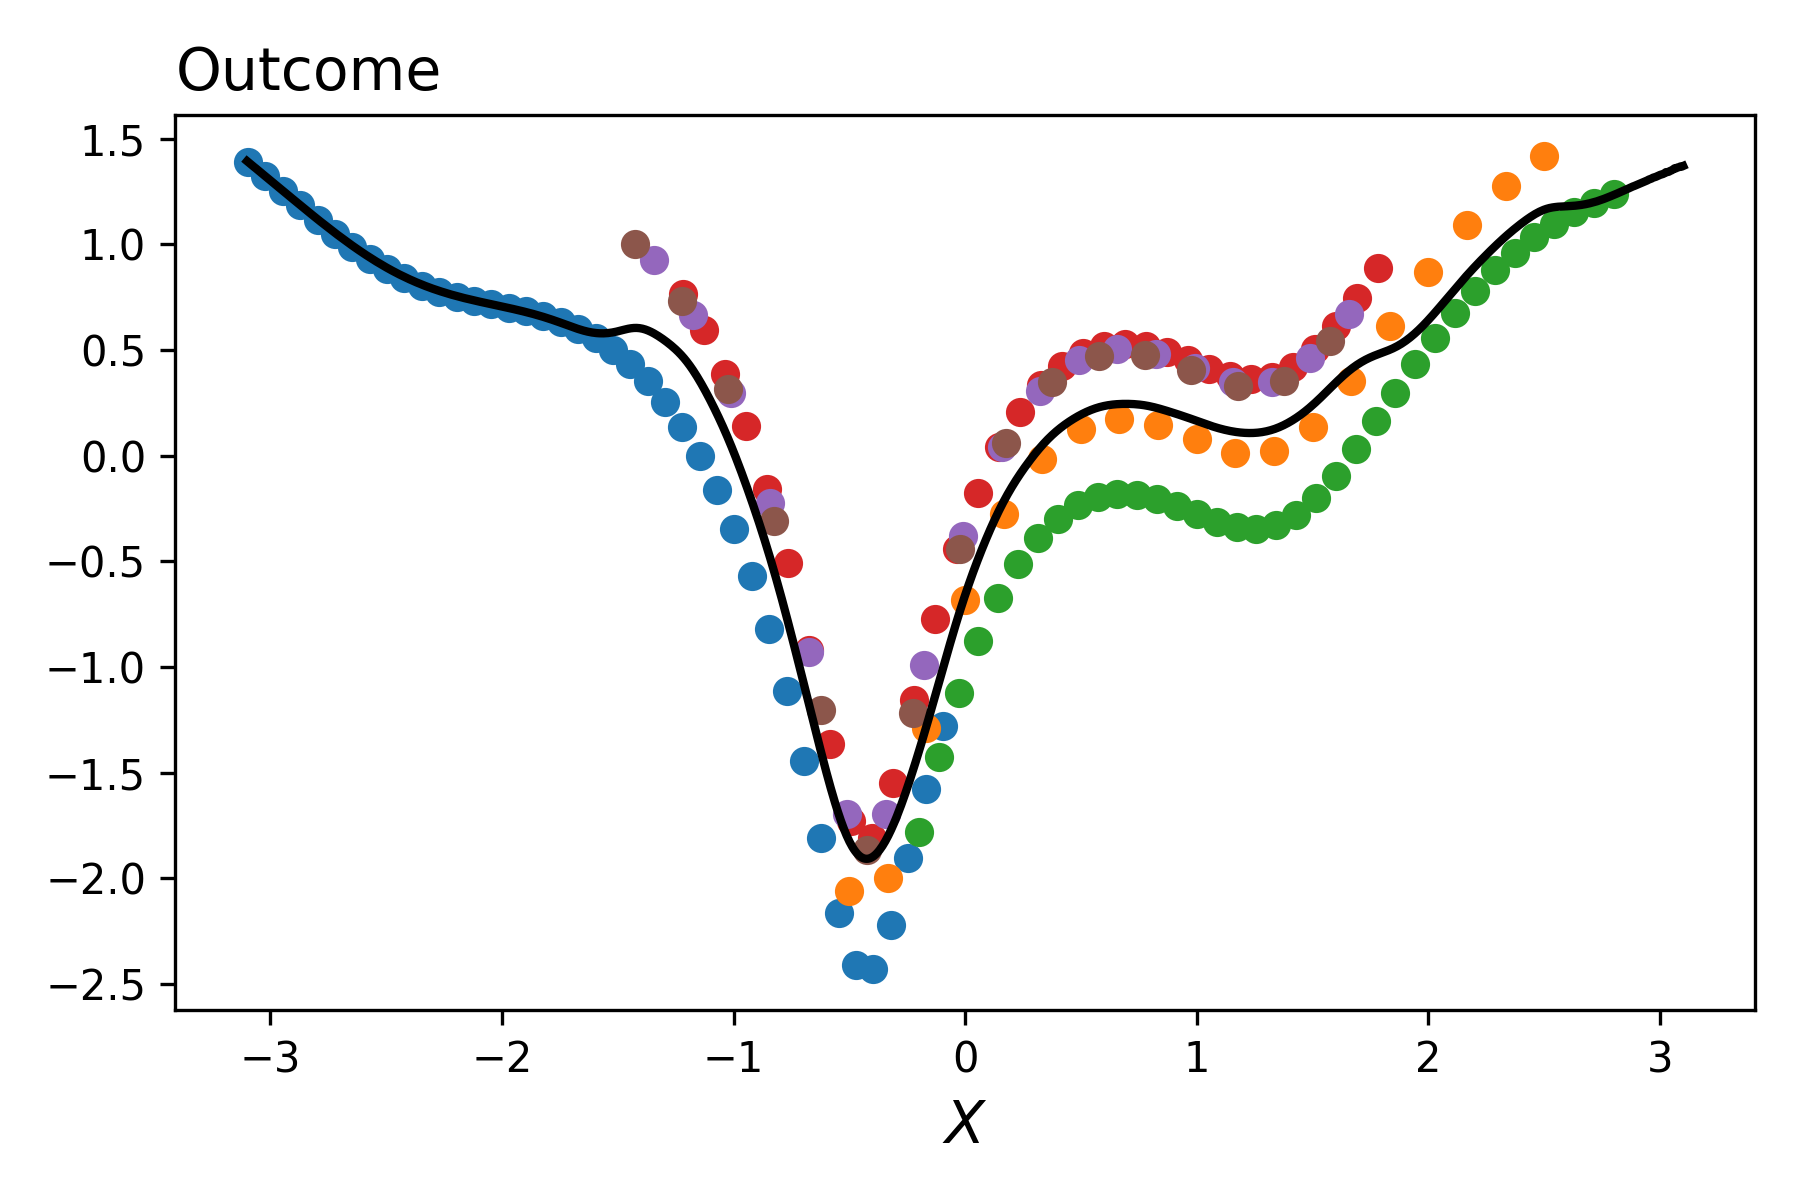
\includegraphics[scale=0.3]{figures/framework/local_linear_no_const_10.0_18_LM.png}
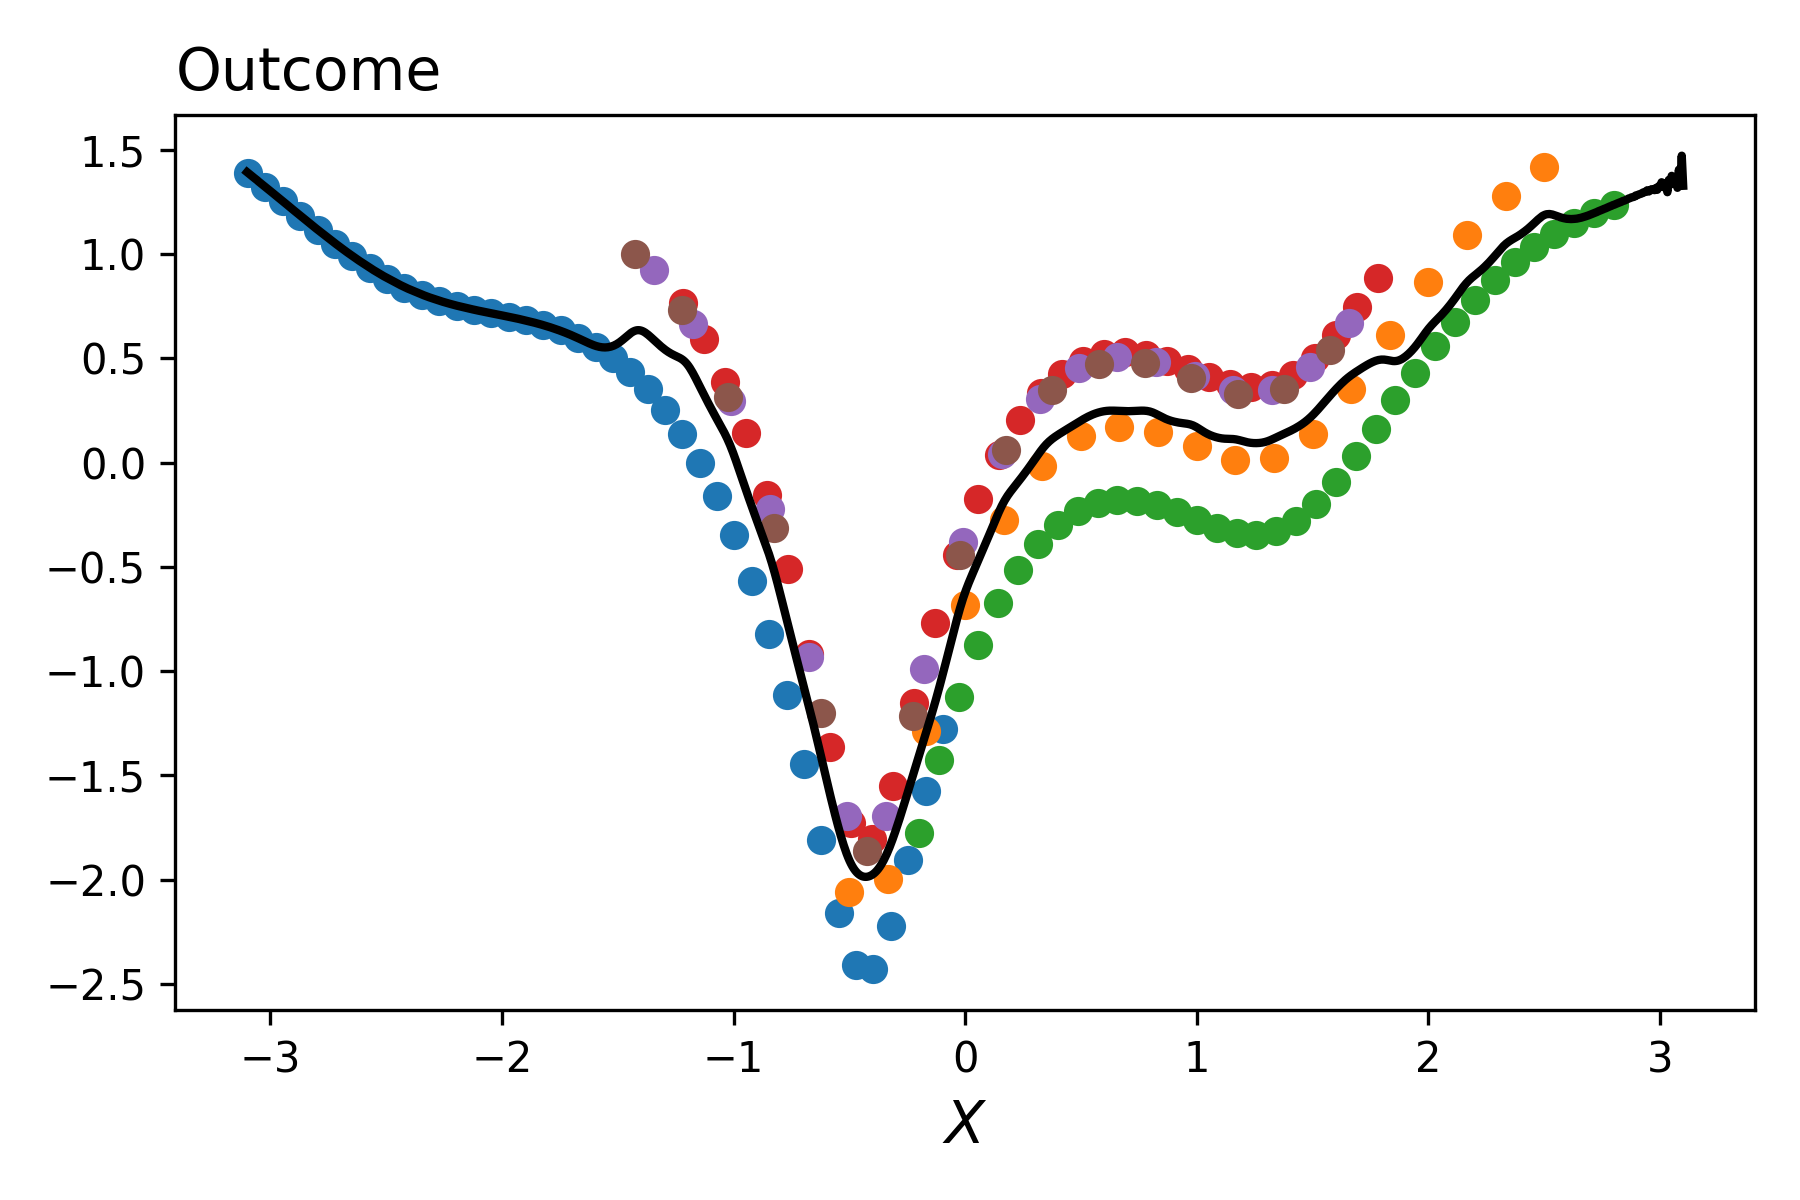
\includegraphics[scale=0.3]{figures/framework/local_linear_no_const_15.0_18_LM.png}
\caption{\href{https://github.com/pharringtonp19/rfp/blob/main/notebooks/local_weighted_linear_regression_no_avg_effect_LM.ipynb}{Reproduced Here}}
\label{fig:nonparametrics}
\end{figure}
Our approach is motivated in part by \cite{domingos2020every} which illustrates how neural networks can be understood within the framework of a kernel machine. The insight of the work is that the kernel, the similarity measure $k(x,x')$ can be understood as the inner product of the gradient of the partially evaluated neural network a the corresponding point. While such a relationships holds exactly only in the gradient flow regiem, it suggests that we can locally correct our model for the presence of clustered data in a global manner by adjusting how we take the gradients of the model. 

\begin{align*}
\intertext{Path Kernel}
K(x,x') = \int \Big \langle \nabla _{\theta} f_x\big(\theta(t)\big), \nabla _{\theta}f_{x'}\big(\theta(t)\big) \Big\rangle dt \\ 
\intertext{Model}
K_{\theta}(x,x') = \int _0^1 \Big \langle \nabla _{\theta} f_x\big(\theta(t)\big), \nabla _{\theta}f_{x'}\big(\theta(t)\big) \Big\rangle dt \\ 
\intertext{Cluster Specific Model}
K_{\theta^*_c(\theta)}(x,x') = K_{\theta}(x,x') + \int _1^{1+ \varepsilon} \Big \langle \nabla _{\theta} f_x\big(\theta(t)\big), \nabla _{\theta}f_{x'}\big(\theta(t)\big) \Big\rangle dt \\ 
\end{align*} 


illustrates that as the learning rate of a neural network approaches the gradient flow regime, the learned model can be represented by a kernel machine with the path kernel.\footnote{Kernel Machines\begin{align*}
    y = g \Big(\sum a_iK(x, x_i) + b \Big) 
\end{align*}} 




In contrast, subject to the appropriate hyperparameters, our method produces a reasonable estimate.

\begin{figure}[htbp]
\centering
\begin{subfigure}{.48\textwidth}
    \centering
    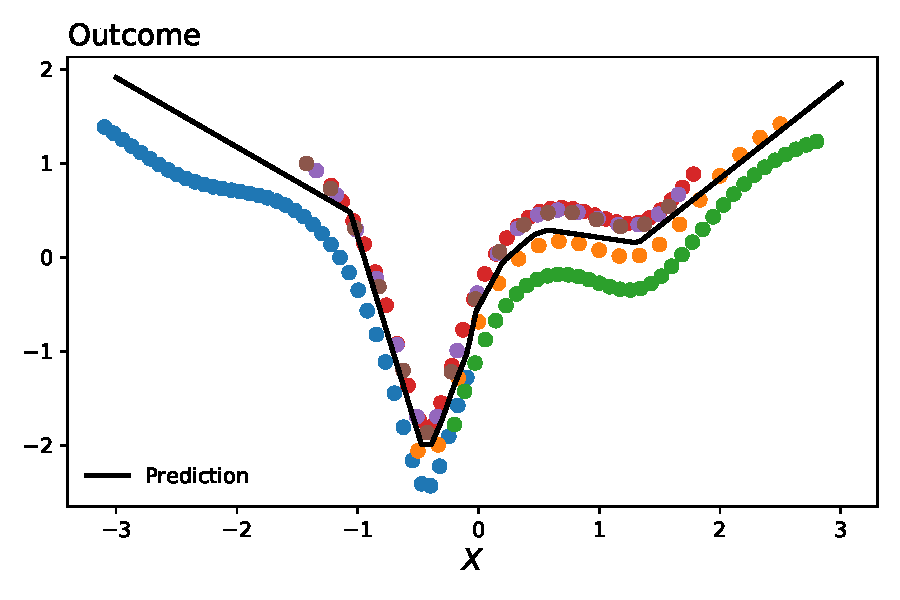
\includegraphics[width=.95\linewidth]{figures/framework/gradient_descent_motivating_example.pdf}
    %\caption{All zip codes}
    %\label{SUBFIGURE LABEL 3}
\end{subfigure}
\begin{subfigure}{.48\textwidth}
    \centering
    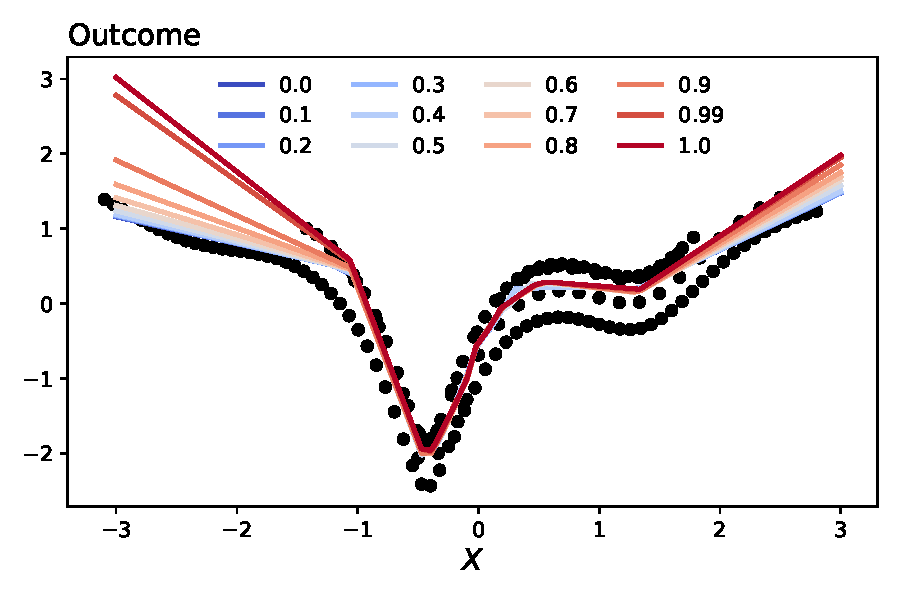
\includegraphics[width=.95\linewidth]{figures/framework/gradient_descent_motivating_example_tune.pdf}
    %\caption{High Eviction Zip Codes}
    %\label{SUBFIGURE LABEL 4}
\end{subfigure}
\caption{The general pattern that these figures try to highlight is that in order to fit the the `v`-shaped valley in the function, the model overfits the tails of the function -- \href{https://github.com/pharringtonp19/jmp_paper/blob/main/notebooks/gradient_descent_motivating_example.ipynb}{Reproduced Here}}
%\label{FIGURE LABEL}
\end{figure}
\subsection{Implicit Cluster Map}
\begin{itemize}
    \item In contrast to linear regression, we do it implicitly 
    \item In contrast to econometric, machine-learning agnostic, we're trying to leverage the success of deep learning models to define what's local. 
\end{itemize}
As mentioned in the introduction, our approach to modern statistical learning theory places less emphasis on understanding the statistical properties of the method (which are difficult to capture in a meaningful way) and more emphasis on the understanding the inductive bias of the algorithm. 
\textbf{TL;DR} In this section, we define our implicit cluster map as a regularized version of the popular gradient based meta-learning MAML.\footnote{Model Agnostic Meta-Learning (MAML), a method that consists of two optimization loops, with the outer loop finding a meta-initialization,
from which the inner loop can efficiently learn new tasks.-- \cite{raghu2019rapid}} While follow-up work such as \cite{raghu2019rapid} has shown that the ``the meta-initialization already providing high quality
representations'', such an analysis assumes a cluster specific head of the network. We show that empirically, without this cluster specific head, the meta-initialization is not done in the right space which motivates our need to add an additional form of regularization.

As applied microeconomists, we are accustomed to writing our problem as a bi-level optimization problem so as to better distinguish between the parameters of interest and the nuisance parameters. In this context, the nuisance parameters are cluster specific parameters that are ``fit'' during the inner optimization process. Below, we follow the language used by \cite{belkin2021fit} in distinguishing between classical and modern estimation techniques.
 
\begin{align*}
    \mathcal{L}(\theta) &:= \sum _c \mathcal{L}_c(\theta), \quad \mathcal{L}_c(\theta) := G(\theta, \theta^*_c(\theta)), \quad  \theta_c^*(\theta) := \underset{\theta_c}{\textrm{argmin}} \ F(\theta, \theta_c) 
\end{align*}

With “Classical” under-parameterized models, as in the case of linear regression, $F$, the clustere-specific empirical loss function is exactly what you would expect. 
\begin{align*}
    F(\theta, \theta_c^*(\theta)) := \sum _{i \in c}\big(y_i - \theta^Td_i - \theta _c^*(\theta)^Tx_i \big)^2
\end{align*}
 With“Modern” over-parameterized models, though, like the ones that we target in this paper, we make the following adjustments. 
 We restrict the objective function that is used to implicitly define the cluster specific maps. First, we generalize the above set-up by allowing the cluster specific parameters to be in one-to-one correspondance with the parameters of interest. Second, we constrain the implicit cluster function $\theta_c^*(\theta)$. Without some form of regularisation, given the flexibility of neural network models as illustrated in \cite{zhang2021understanding}, the jacobian of this function can easily be zero. We illustrate this concern in figure \ref{fig:Missinggrads}. And finally, we add a penalty term to the cluster specific loss function to ensure that adaptation happens in the right space. 
 

\begin{align*}
\intertext{Define our empirical cluster parameters in relation to the parameters of interest}
    G(\theta) &:= \sum _{i \in c}\big(y_i - f(\theta_c^*(\theta), x_i)\big)^2
\intertext{Implicit Cluster Map}
\theta_c^*(\theta) &:= \theta^t - \alpha \nabla_{\theta}G(\theta^{t-1}), \quad \theta^{0} = \theta 
\intertext{As well as introduce an auxilliary term to the cluster specific loss function}
    \mathcal{L}_{c}(\theta) &:= G(\theta) + H(\textrm{Path}(\theta, \hat{\theta}^*_c(\theta)))
\end{align*}
We illustrate the relative importance of our design choices in figure \ref{fig:mamlablation}. In figure \ref{fig:overfittails} we see that supverized learning overfits to the clusters in the tails of their distributions. In figure \ref{fig:wrongspace}, we see that MAML meta initialization is in the wrong space. And finally in figure \ref{fig:rfp}, we see that a regularized version of MAML appears to learn something reasonable. 
\begin{figure}[htbp]
\centering
\begin{subfigure}{.32\textwidth}
    \centering
    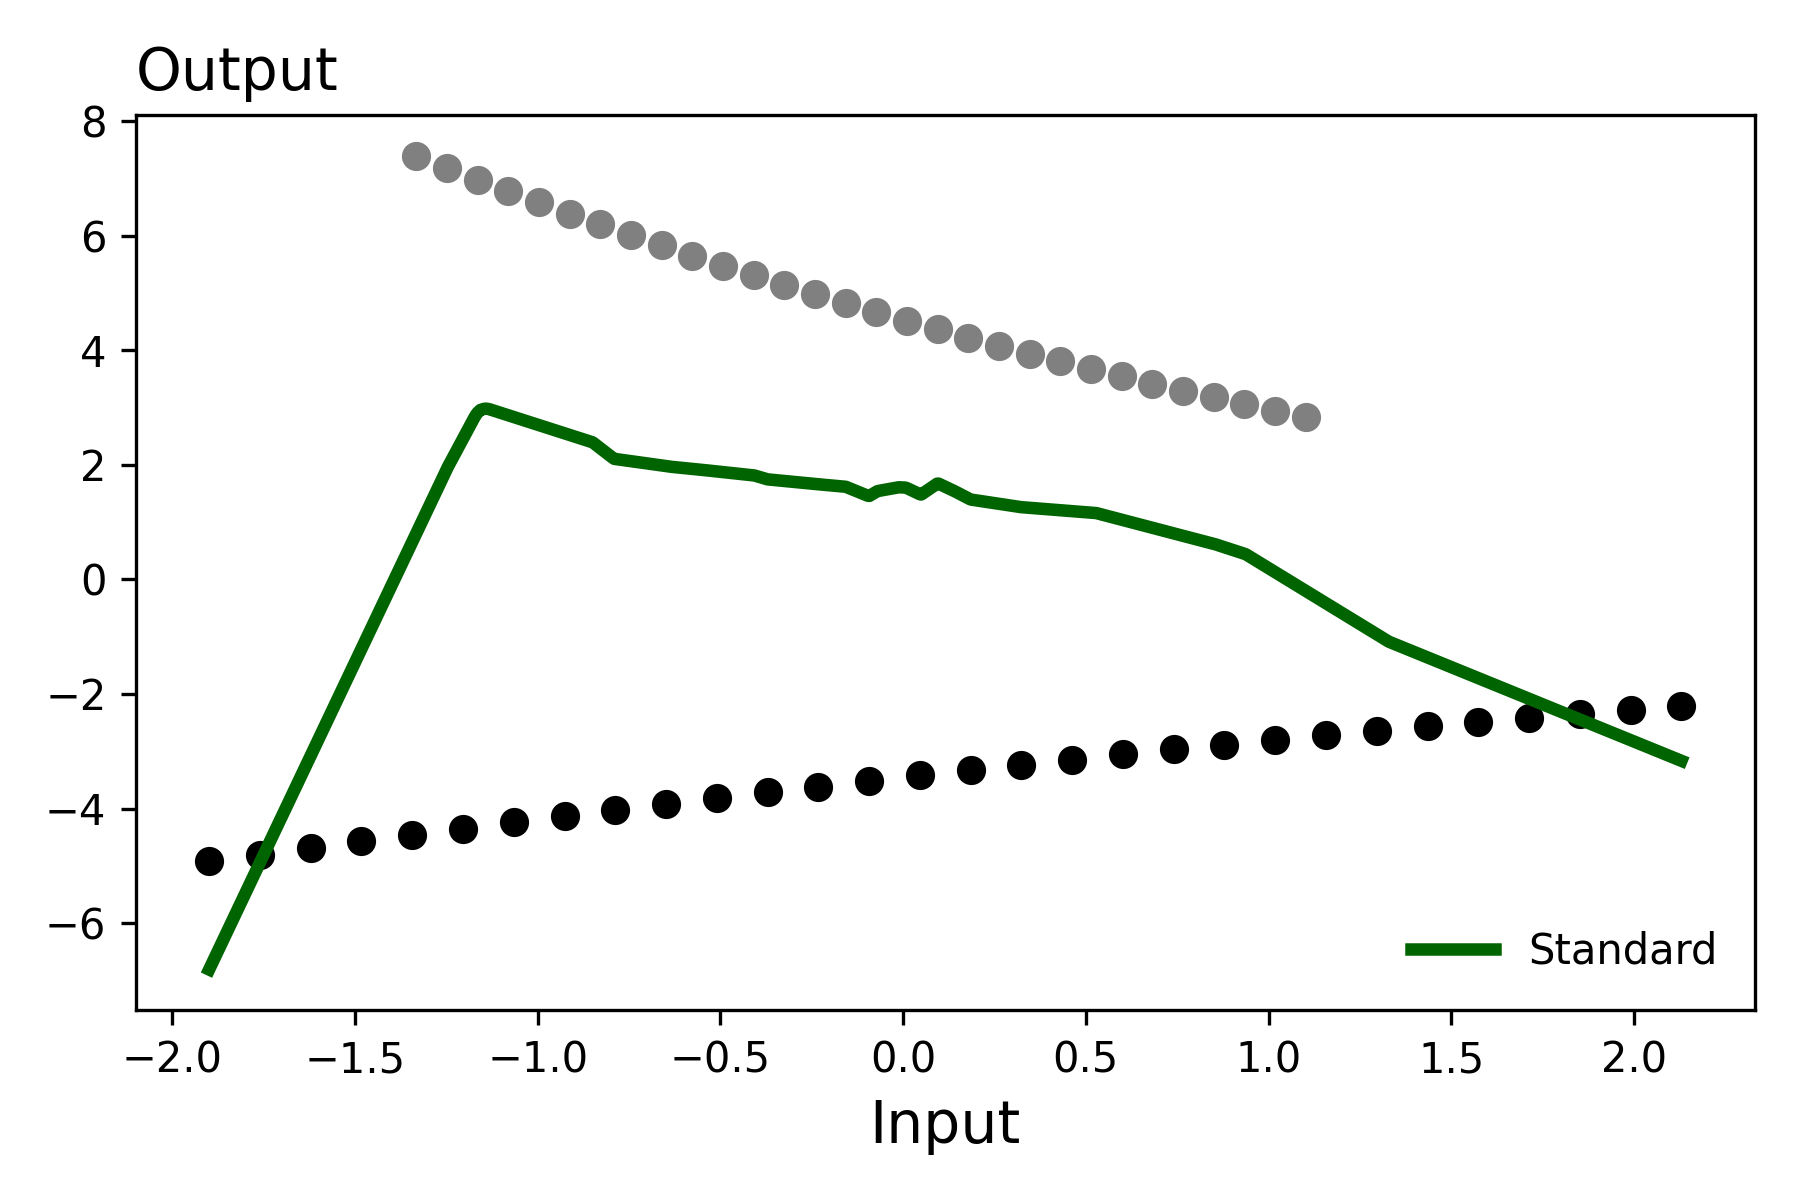
\includegraphics[width=.95\linewidth]{figures/framework/grad_desc_toy_Standard.png}
    \caption{Standard Training}
    \label{fig:overfittails}
\end{subfigure}
\begin{subfigure}{.32\textwidth}
    \centering
    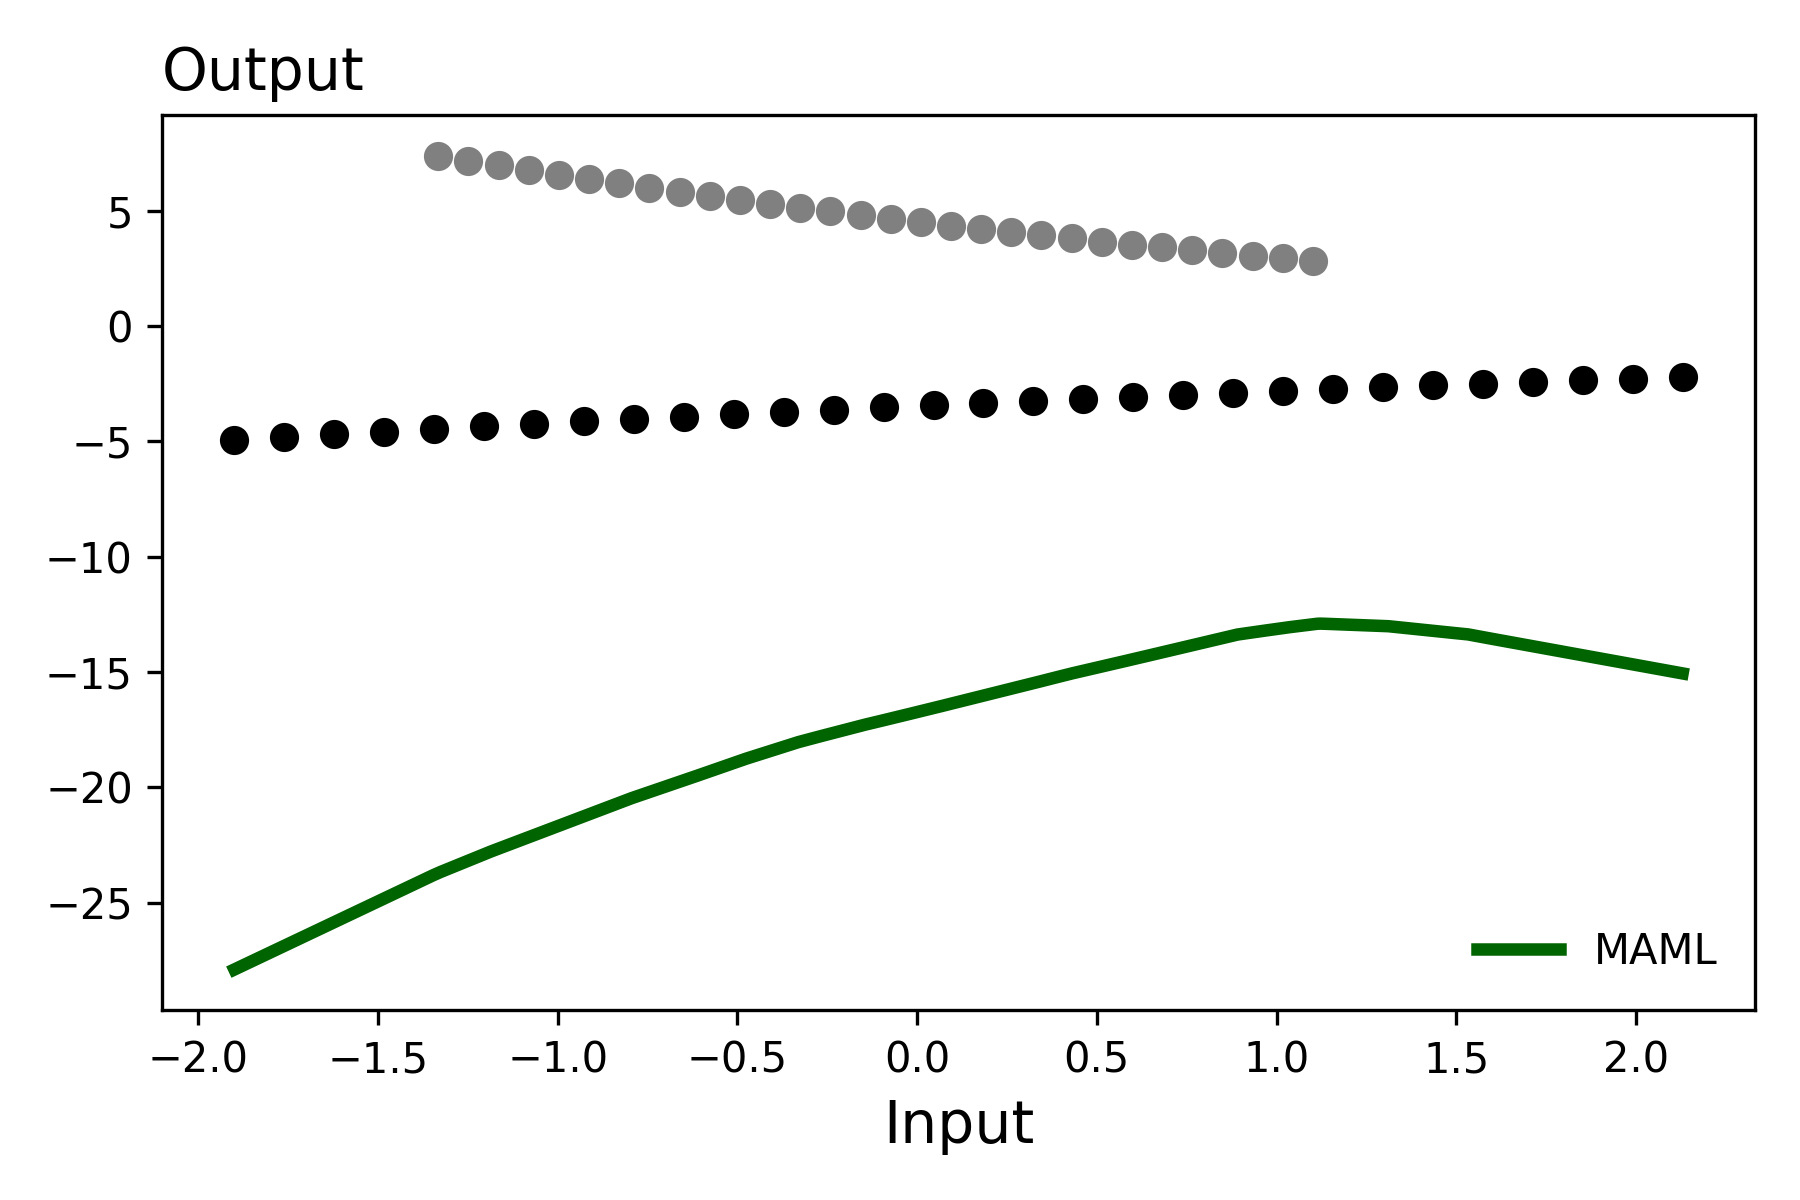
\includegraphics[width=.95\linewidth]{figures/framework/grad_desc_toy_MAML.png}
        \caption{MAML}
    \label{fig:wrongspace}
\end{subfigure}
\begin{subfigure}{.32\textwidth}
    \centering
    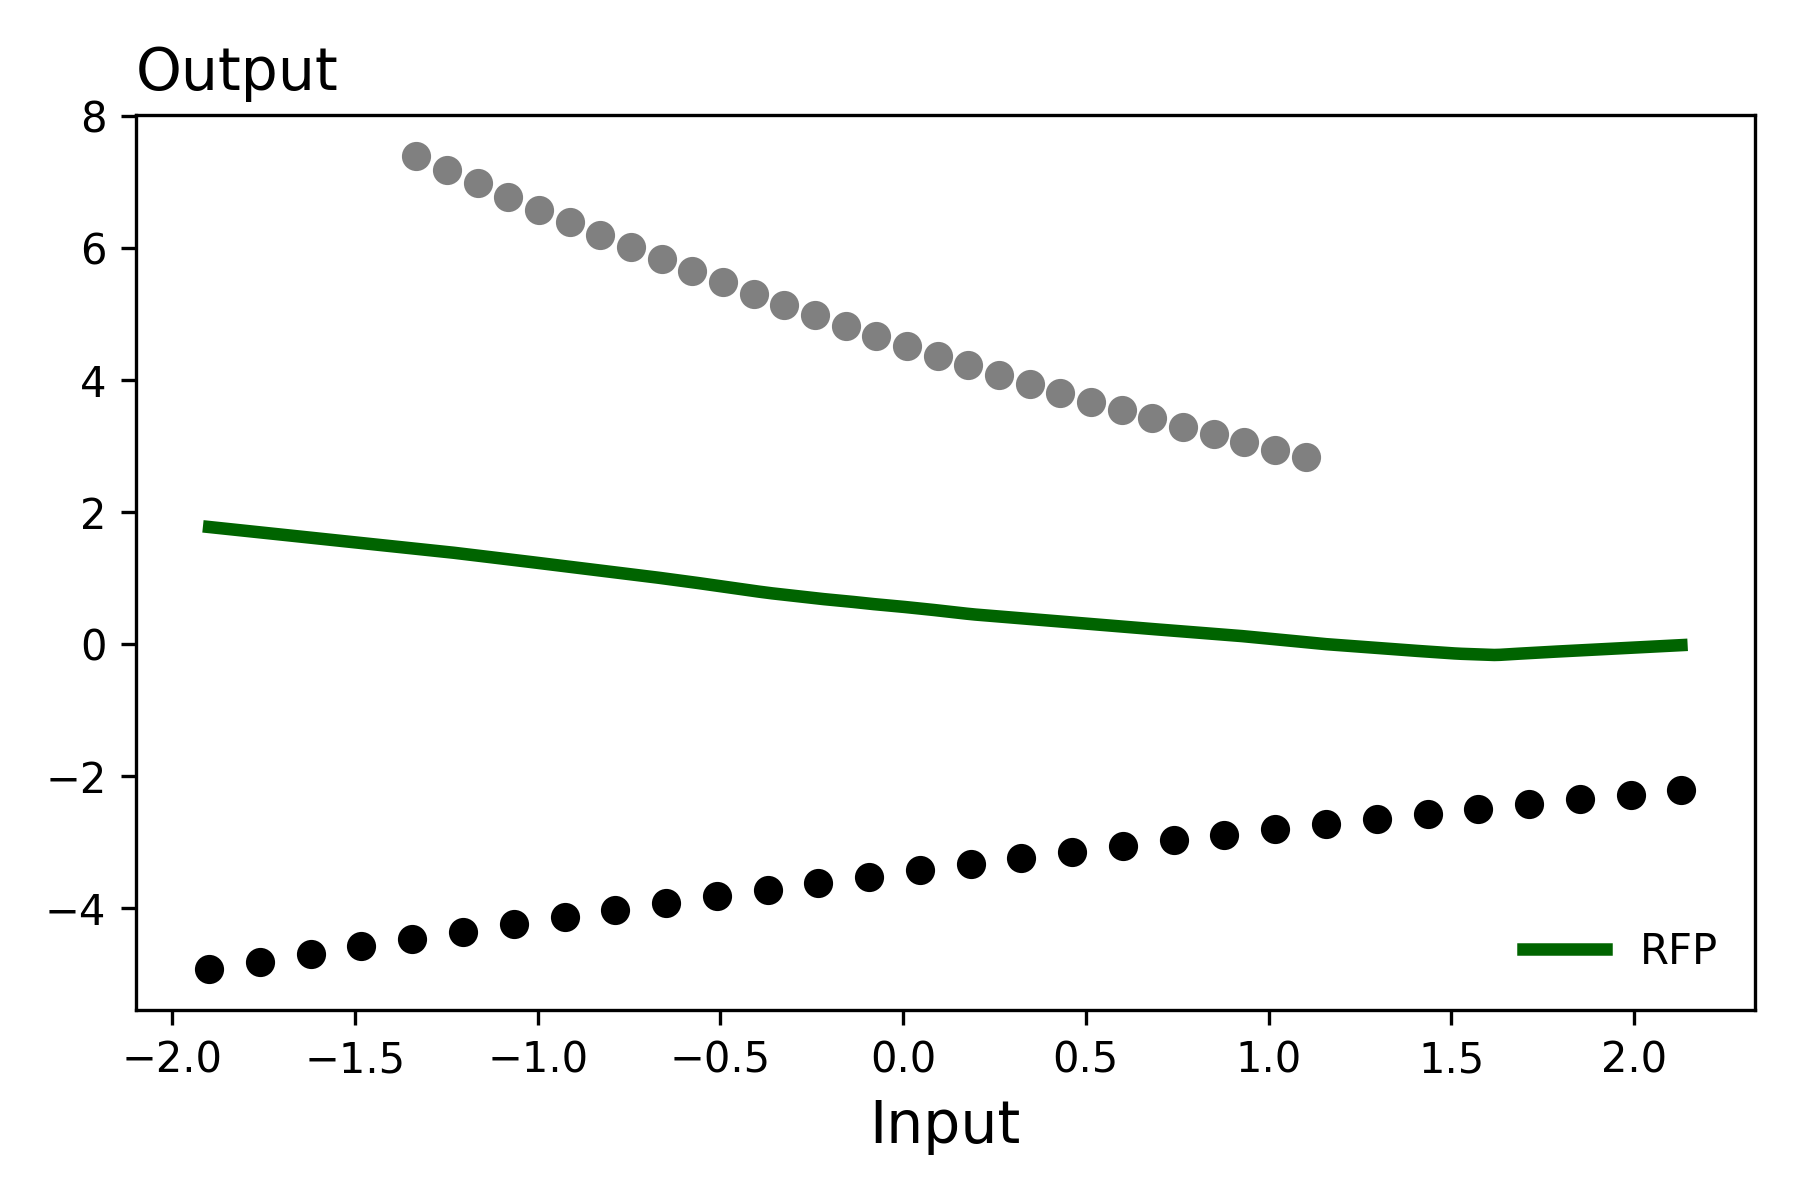
\includegraphics[width=.95\linewidth]{figures/framework/grad_desc_toy_RFP.png}
        \caption{RFP}
    \label{fig:rfp}
\end{subfigure}
\caption{ \href{https://github.com/pharringtonp19/rfp/blob/main/notebooks/grad_desc_toy.ipynb}{Reproduced Here}: The grey and black dots represent data from separate clusters. Each figure corresponds to fitting a neural network to this data under different training algorithms}
\label{fig:mamlablation}
\end{figure}

\begin{figure}[htbp]
\centering
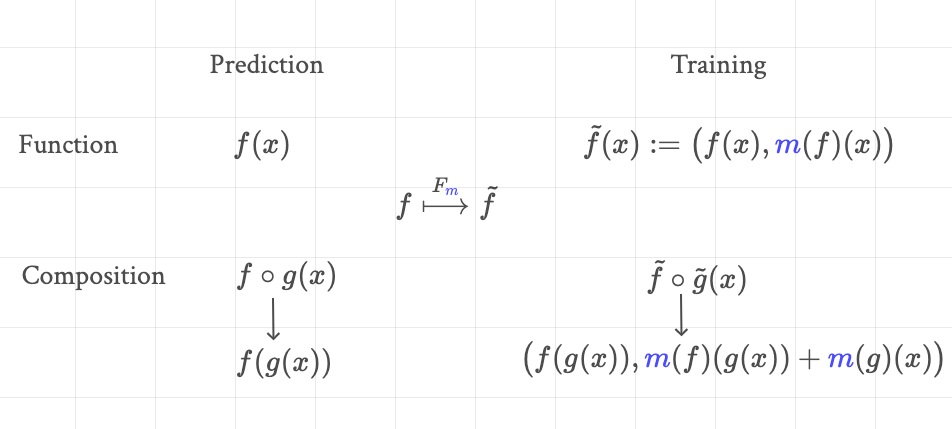
\includegraphics[width=0.8\textwidth]{figures/framework/cat.png}
        \caption{High Level Summary}
        \label{fig:hls}
\end{figure}

Such an approach is inspired/related by proximal methods (\cite{parikh2014proximal}).\footnote{Note that the codomain of $f$ is taken to be $\mathcal{R} \cup \{ \infty\}$, while the domain are set of inputs that take finite values.} Which can be thought of as generalized projections, as well as gradient steps. 


 


\section{Toy Model}
We write down the following model in order to clarify our estimand of interest. The key detail is that we parameterize the ``consumer's'' constraint function with a variable that denotes the status of the Right to Counsel (where 1 means in the policy is in effect, and 0 means it is not). We allow the parameters of the constraint and utility functions to differ across individuals, and define our estimand as the expected value taken with respect to these the probability law induced by these random variables. \textbf{Notationally}, we denote the partial evaluation of a function by subscripting the function with the argument.\par 
We define an element of the choice set as a bundle of housing related features. The first component we include, which is the most relevant to our dataset, is housing search length. It's important to acknowledge that individuals may be substituting across a wide range of housing aspects (such as the price of the house and the quality of the house) among other features. For the purposes of this model, we omit these, as we do not observe these features in the data. 
\begin{align*}
    x := (\textrm{search period}, \textrm{quality}, \textrm{price}, \dots ) \in \mathcal{X}
\end{align*}




As indicated by its signature, we introduce a parameterized constraint function where we allow the parameters to vary across individuals. This constraint function not only incorporates the macroeconomic features of the housing market, but also the effects of the landlords actions/policies towards individual tenants.
\begin{align*}
   F :: \textrm{Params} \to  \textrm{RTC} \to \mathcal{X} \to \{0, 1\} %Shomik: This formulation seems unclear to me.
\end{align*}
The utility function then captures the value of each housing option. 
\begin{align*}
U :: \textrm{Params} \to \mathcal{X} \to \mathcal{R}_+ 
\end{align*}

%================
%Shomik: I think instead of saying params, we should put some notation. Like H (for housing) or something). Makes it a bit cleaner IMO. Or is that what you're using P for later? Then make it P from the get go.

%
%=====================
With the essential components of the model defined, we can express the individual choice problem as follows. The following problem would model an individual not in a treated zip code or prior to the policy implementation as the second parameter of the constraint function takes the value $0$. The pre-image of $0$ under the constraint function defines the feasibility set. 
\begin{align*}
\underset{x \in F_{p, 0}^{-1}(0)}{\textrm{maximize}} \ U_{\alpha} (x)
\end{align*}
Via-this parameterized optimization problem, we can then define the implicit function of interest which captures the effects of the individual-level parameters and the policy on the search length. 
\begin{align*}
s^*(\textrm{rtc}, p, \alpha) := \underset{x \in F_{p, \textrm{rtc}}^{-1}(0)}{\textrm{argmax}_0} \ U_{\alpha} (x) \\ 
\end{align*}
As we are only interested in the later effects, we integrate over the individual-level parameters leading to the estimand defined below.
\begin{align*}
&\theta := \mathbb{E}[s^*(1, p, \alpha) - s^*(0,  p, \alpha)] \\
&\quad = \int _{\Omega} s^*\big(1, p, \alpha\big) - s^*\big(0, p, \alpha\big)d\mathbb{P}
\end{align*}

 
%Shomik: We need a conclusion to this. Say what it is and why.




\section{Empirical Strategy}
The following notation defines the key variables used in the estimators defined below. 
\begin{align*}
    &Y_i:  \textrm{Search Duration}\\
    &X_i: \textrm{Age, Gender, Race, Family Size}\\ 
    %&P_i: \textrm{Rapid Rehousing Provider}\\ 
    &Z_i: \textrm{Zip Code} \\
    &D_i: \textrm{Treated Zip Code}
\end{align*}
\textbf{Note}: Subscripts on the outcome corresponding to subsets of individuals who are observed in that corresponding time period. 

\subsection{Difference-in-Difference}

%Thought: Change Y_i to Y_id (maybe?) where d is the number of days. Not t because that will give the wrong impression.
We fit the following difference-in-difference estimator. In this specification and for the ones that follow, $Y_i$ is a binary variable that indicates whether the search length was less than some specified number of days. We run multiple regressions where we vary what this cutoff is, be it ten, twenty, or sixty days. These results are illustrated in figure \ref{fig:diff_mean}, where we run a number of Difference-in-Difference regressions by changing the cutoff point and graphing the estimates. As we can see the percentage point effect of the Right to Counsel (the y-axis) is relatively constant as we vary the acceptable move-in-date threshold.

%=================
%What's the best way of saying what this means and why we should care?

%We need some of the tables at a specific value. Like a standard regression table of the diff in diff at some cutoff values. Both for the appendix and your presentation (if you can swing it)
%=================
\begin{align*}
    \beta_0 &= \mathbb{E}[Y_1 -Y_0 \mid D=1] -  \mathbb{E}[Y_1 - Y_0 \mid D=0] \end{align*}
Importantly, when we restrict the sample to only high eviction zip codes in figure \ref{fig:diff_mean_high}, we see a relatively consistent negative effect on the probability of moving into housing by a certain date.
\begin{figure}[htbp]
\centering
\begin{subfigure}{.48\textwidth}
    \centering
    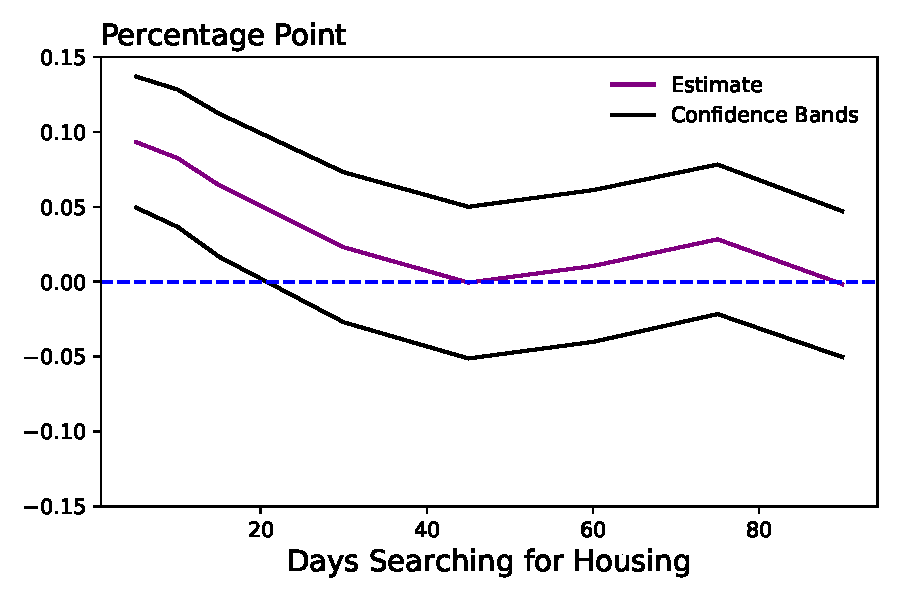
\includegraphics[width=.95\linewidth]{figures/rtc/results/cceh/diff_in_mean_False_False.pdf}
    \caption{All zip codes}
    \label{SUBFIGURE LABEL 3}
\end{subfigure}
\begin{subfigure}{.48\textwidth}
    \centering
    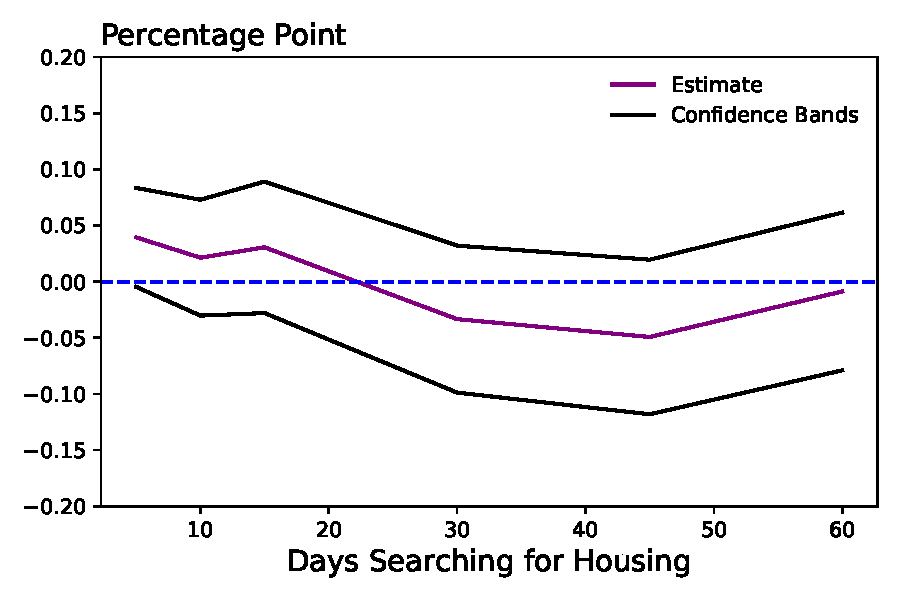
\includegraphics[width=.95\linewidth]{figures/rtc/results/cceh/diff_in_mean_True_False.pdf}
    \caption{High Eviction Zip Codes}
    \label{fig:diff_mean_high}
\end{subfigure}
\caption{ \href{https://github.com/pharringtonp19/evictions/blob/main/scripts/cceh/primary/diff_n_mean_rrh.py}{Reproduced Here}: Confidence Bands formed via stratified bootstrapped sampling without replacement with a $75\%$ sampling rate.)}
\label{fig:diff_mean}
\end{figure}

\subsection{Difference-in-Difference with Controls}
Adding individual level controls as well as zip code fixed effects makes a material difference for the magnitude of the effect but not the sign when we again restrict the sample to high eviction zip codes in figure \ref{fig:diff_control_high}.

%Shomik: My dumb ass says that this is impacting the signs since the estimates are more consistently negative. We need to say why this is happening and what that means.

\begin{align*}
    Y_i &= \alpha _0 + \beta_0 \textrm{Post}_i \times \textrm{Treated}_i + \beta_1  \textrm{Post}_i + \beta_2 \textrm{Treated}_i \\ 
    &\quad + \beta _3X_i + \beta_4 Z_i + \varepsilon_i
\end{align*}
\begin{figure}[htbp]
\centering
\begin{subfigure}{.48\textwidth}
    \centering
    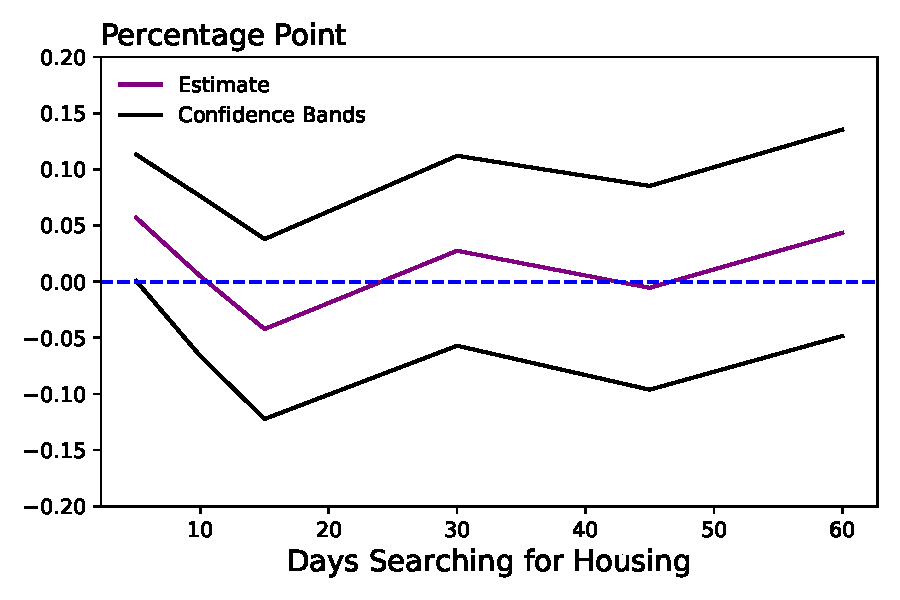
\includegraphics[width=.95\linewidth]{figures/rtc/results/cceh/linear_reg_False_False.pdf}
    \caption{All zip codes}
    \label{SUBFIGURE LABEL 3}
\end{subfigure}
\begin{subfigure}{.48\textwidth}
    \centering
    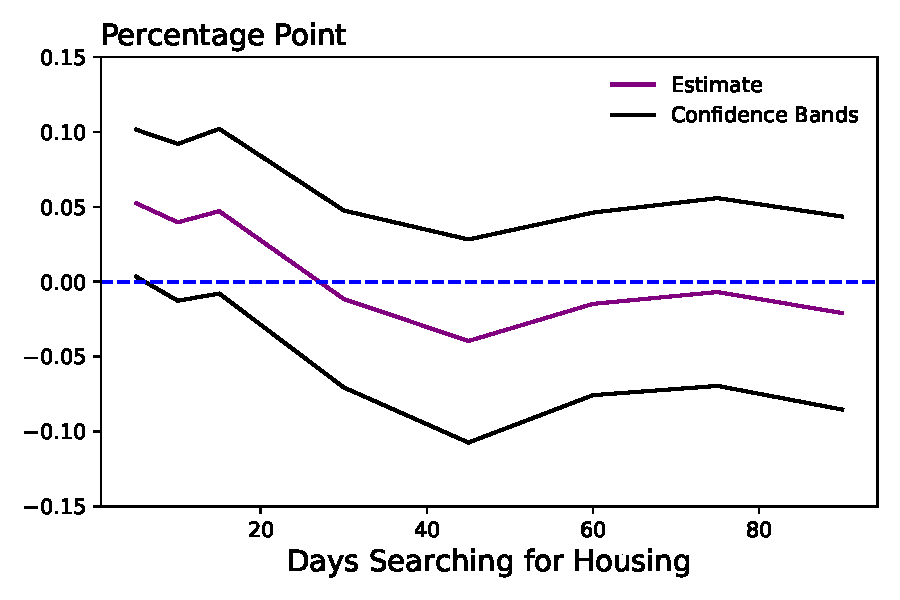
\includegraphics[width=.95\linewidth]{figures/rtc/results/cceh/linear_reg_True_False.pdf}
    \caption{High Eviction Zip Codes}
\label{fig:diff_control_high}
\end{subfigure}
\caption{ \href{https://github.com/pharringtonp19/evictions/blob/main/scripts/cceh/primary/diff_n_mean_rrh.py}{Reproduced Here}: Confidence Bands formed via stratified bootstrapped sampling without replacement (75\%)}
\label{fig:diff_control}
\end{figure}

%\subsection{Partially Linear Difference-in-Difference}

\subsection{Regularizing the Forward Pass}
It's possible to re-write the difference-in-difference model with controls as a linear version of the following estimator. Doing to we see that there are two potential concerns. The first is that the model fails to correct for the propensity score which as highlighted in figure \ref{fig:DML} can be problematic in certain contexts.  

\begin{align*}
\tilde{Y}_i - \mathbb{E}[ \tilde{Y}_i | X_i] = \beta_0 \big(D_i - \mathbb{E}[D_i |X_i]\big) + \varepsilon_i, \quad \textrm{where} \ \tilde{Y}_i =  Y_{1i} - Y_{0i} 
\end{align*}
\begin{comment}

\begin{figure}[htbp]
\centering
\begin{subfigure}{.48\textwidth}
    \centering
    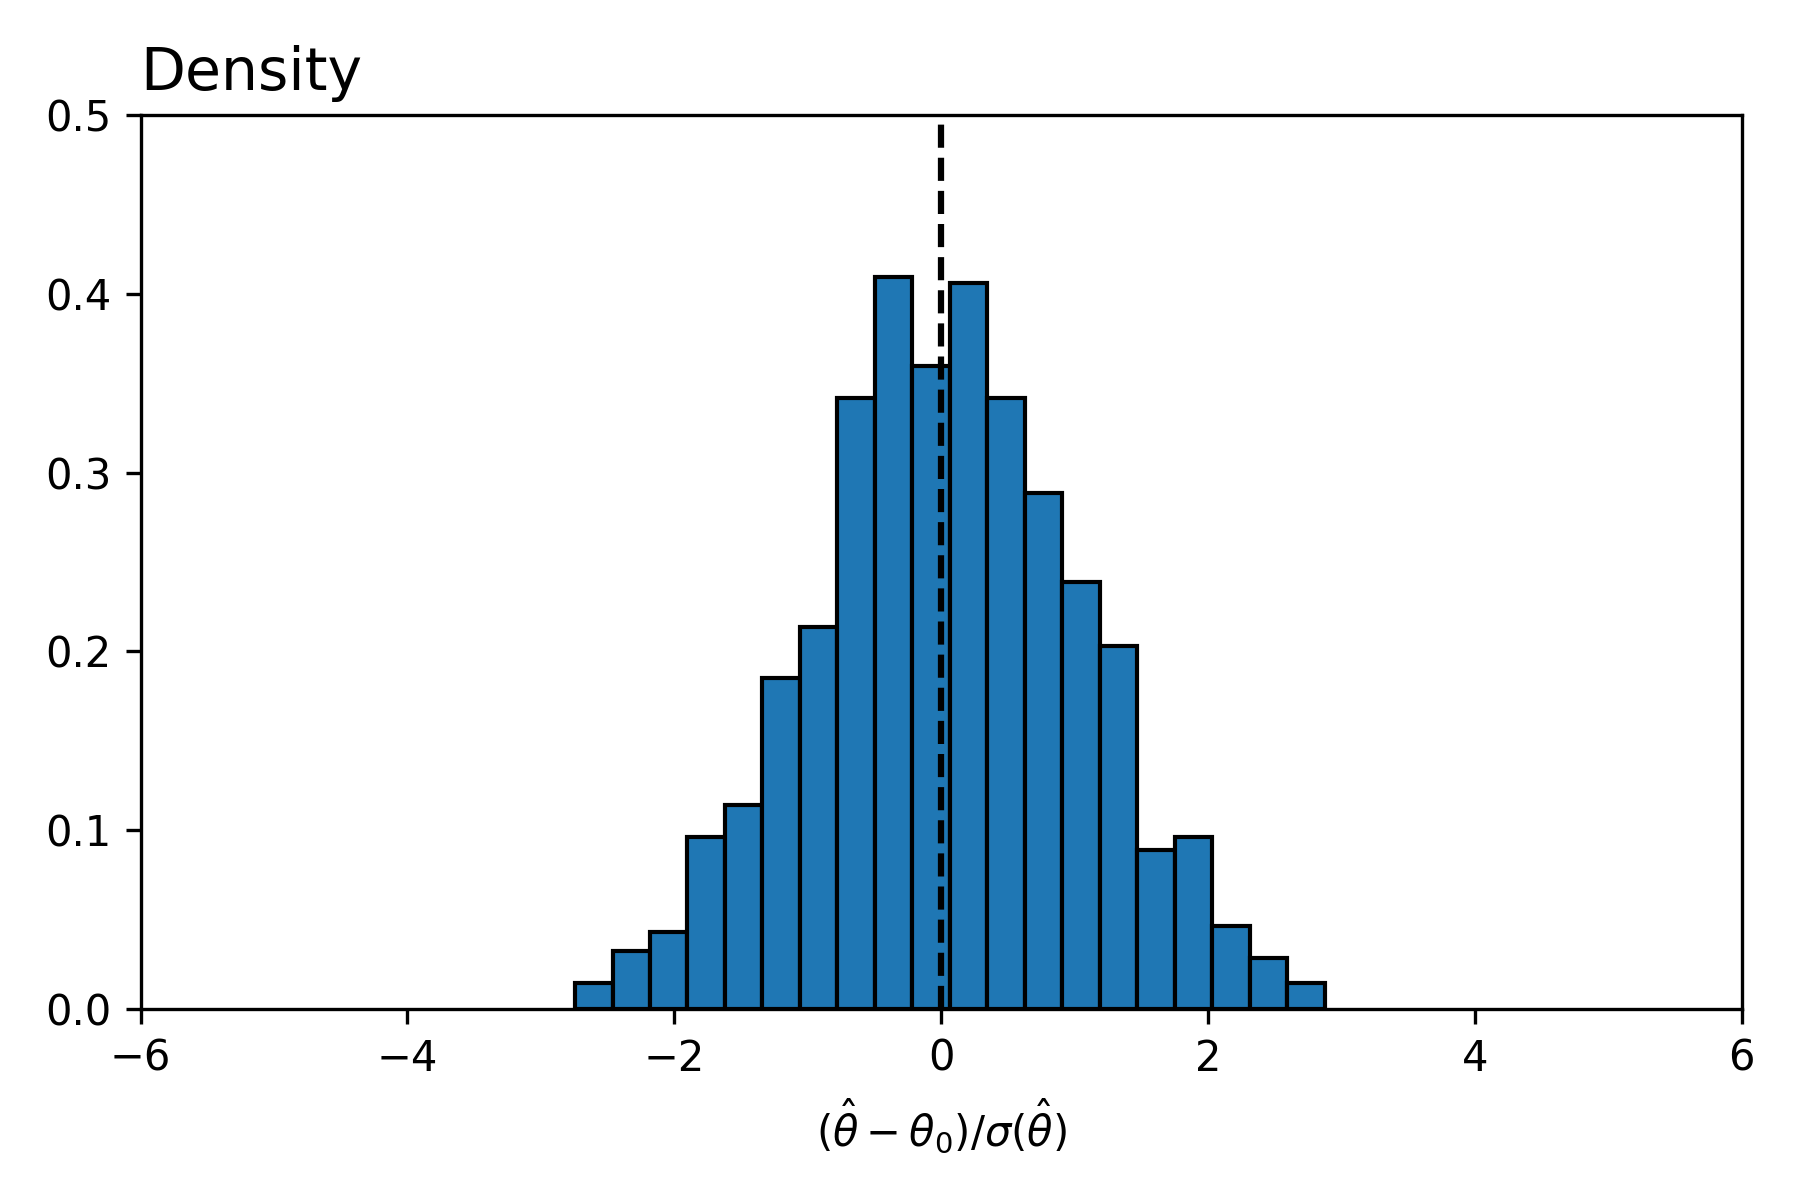
\includegraphics[width=.95\linewidth]{figures/framework/dml_True.png}
    \caption{Original Paper}
    %\label{SUBFIGURE LABEL 3}
\end{subfigure}
\begin{subfigure}{.48\textwidth}
    \centering
    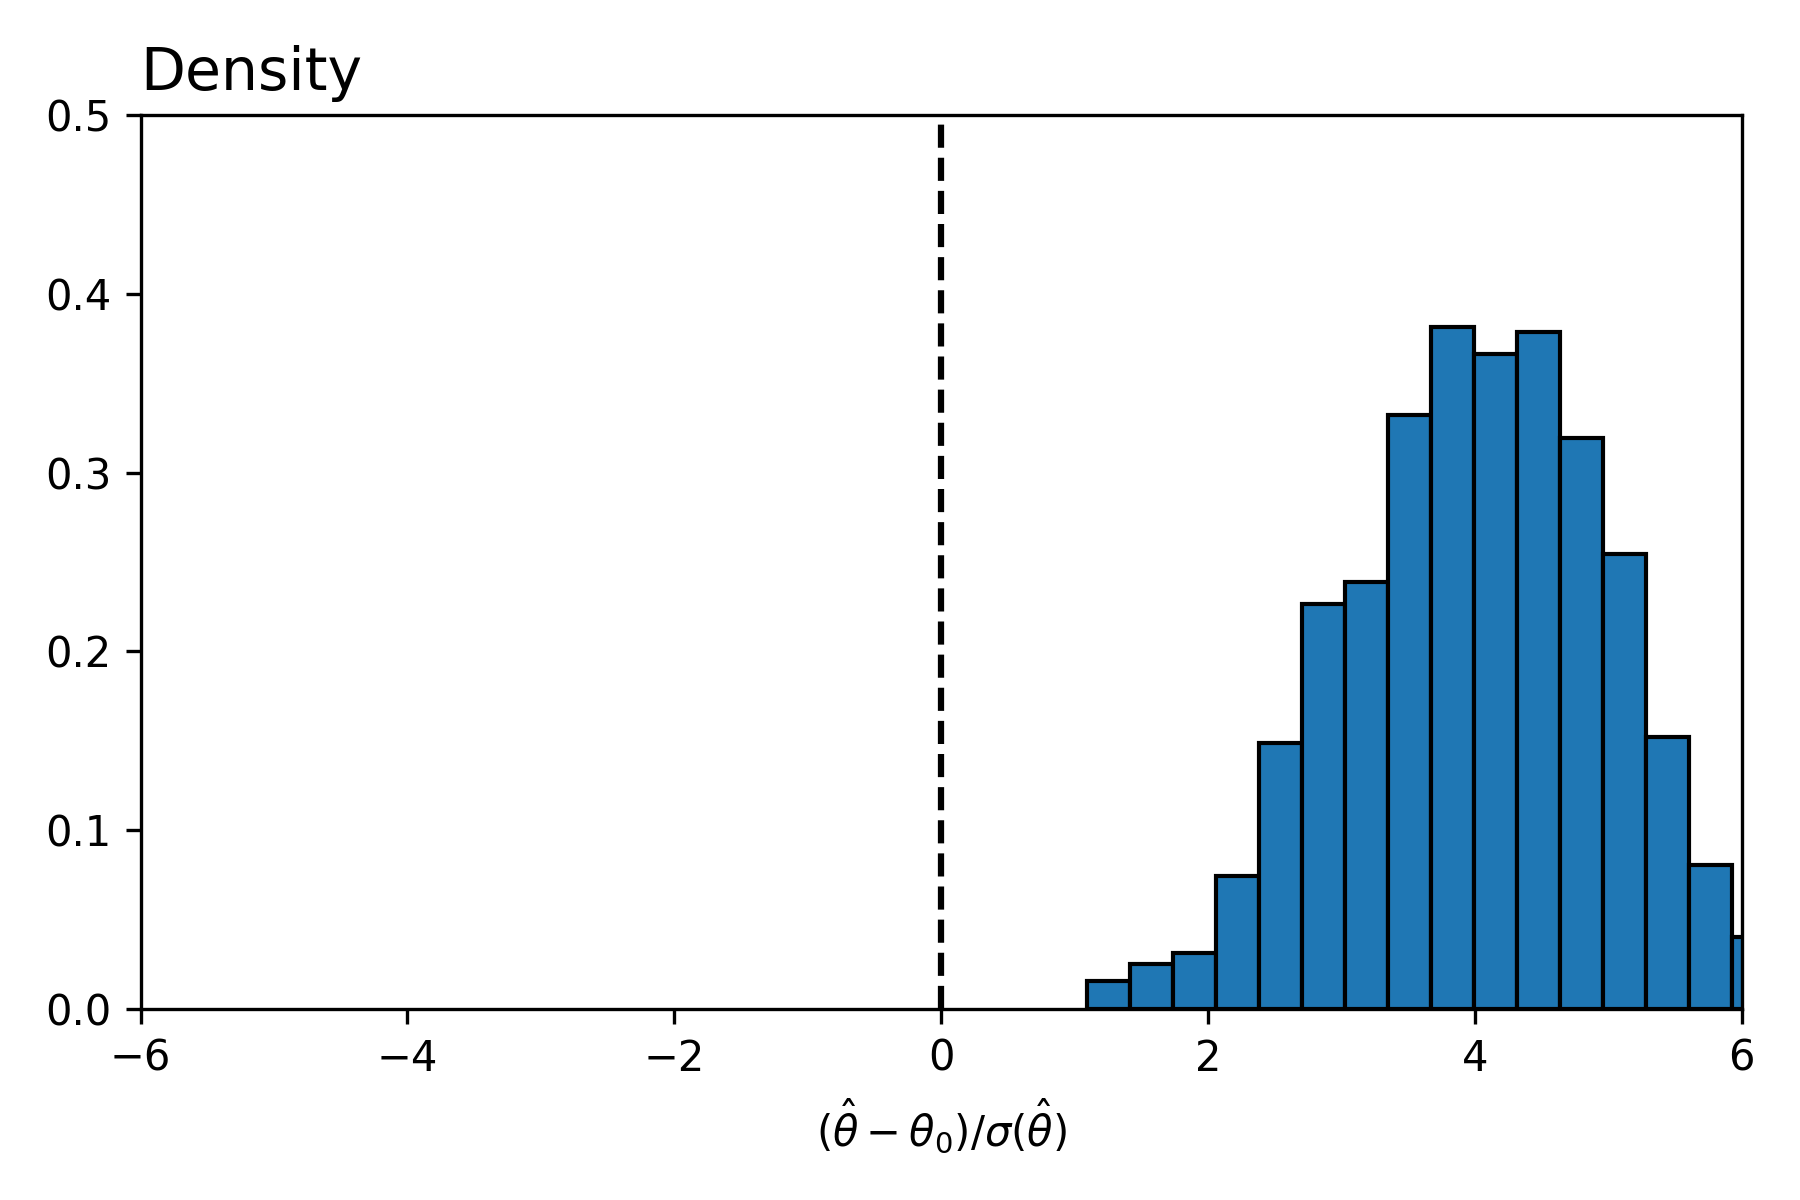
\includegraphics[width=.95\linewidth]{figures/framework/dml_False.png}
        \caption{Nonuniform Propensity Score}
    %\label{SUBFIGURE LABEL 4}
\end{subfigure}
\caption{ \href{https://github.com/pharringtonp19/rfp/blob/main/examples/scripts/dml.py}{Reproduced Here}: The sampling distribution of a Double Machine Learning Based Neural Network Estimator under selection on observables. In (a), we replicate the results of the original paper where the authors assume a constant treatment effect. Under a non-constant treatment effect as captured in (b), a failure to correct for the propensity score can introduce bias.}
\label{fig:DML}
\end{figure}
\end{comment}
The natural correction is to then deploy a fully-nonparametric model. 
\begin{align*}
\beta_0 := \int \mathbb{E}[\tilde{Y}_i | X_i, D_i=1] - \mathbb{E}[\tilde{Y}_i | X_i, D_i=0] d\mathbb{P}_X
\end{align*}
As previously illustrated, though, when treatment varies at the cluster level such estimators are susceptible to the tragic triad. We therefore implicitly partiall out the cluster effects by fitting these conditional expectations using our regularized forward pass framework which generates the results captured in figure \ref{fig:rfp_results}. Note, in order to limit the computation burden of these models we fit the following model. The only difference is that it removes the first step of estimating $\tilde{Y}$. 

\begin{align*}
    \beta _0 := \int d\mathbb{P}_X\Big(\big(\mathbb{E}[Y_1 |X,D=1] - \mathbb{E}[Y_0 |X,D=1]\big) -  \big(\mathbb{E}[Y_1 |X,D=0] - \mathbb{E}[Y_0 |X,D=0]\big)\Big)
\end{align*}

\begin{align*}
\intertext{Cross-Sectional Setting}
    \hat{\theta}_t(X) &:= \mathbb{E}[Y_{it} |X_{it}, D_{it}=1, C_{it} \in A] - \mathbb{E}[Y_{it} |X_{it}, D_{it}=0, C_{it} \in A^c] \\ 
    &= \mathbb{E}[Y_{it}(1) |X_{it}, C_{it} \in A] - \mathbb{E}[Y_{it}(0) |X_{it}, C_{it} \in A^c] \\ 
\intertext{Repeated Cross-Sectional Setting}
    \hat{\theta}(X) &:=     \hat{\theta}_t(X)  - \hat{\theta}_{t-1}(X)  \\ 
    &= \mathbb{E}[Y_{t}(1) - Y_{t-1}(0)|X, C \in A] -  \mathbb{E}[Y_{t}(0) - Y_{t-1}(0)|X, C \in A^c] \\ 
    &= \mathbb{E}[Y_{t}(1) - \textcolor{blue}{Y_{t}(0)}|X, C \in A] \\ 
    &+ \underbrace{ \mathbb{E}[\textcolor{blue}{Y_{t}(0)} - Y_{t-1}(0)|X, C \in A] -  \mathbb{E}[Y_{t}(0) - Y_{t-1}(0)|X, C \in A^c]}_{\approx 0 } \\ 
    &= \mathbb{E}[Y_{t}(1) -  Y_{t}(0)|X, C \in A], \quad \quad  \textrm{Local Treatment Effect on the Treated} \\ \\
\hat{\theta} &:= \int \hat{\theta}(X)d\mathbb{P}_X, \quad \quad  \textrm{Average Treatment Effect on the Treated}
\end{align*}


\begin{figure}[htbp]
\centering
\begin{subfigure}{.48\textwidth}
    \centering
    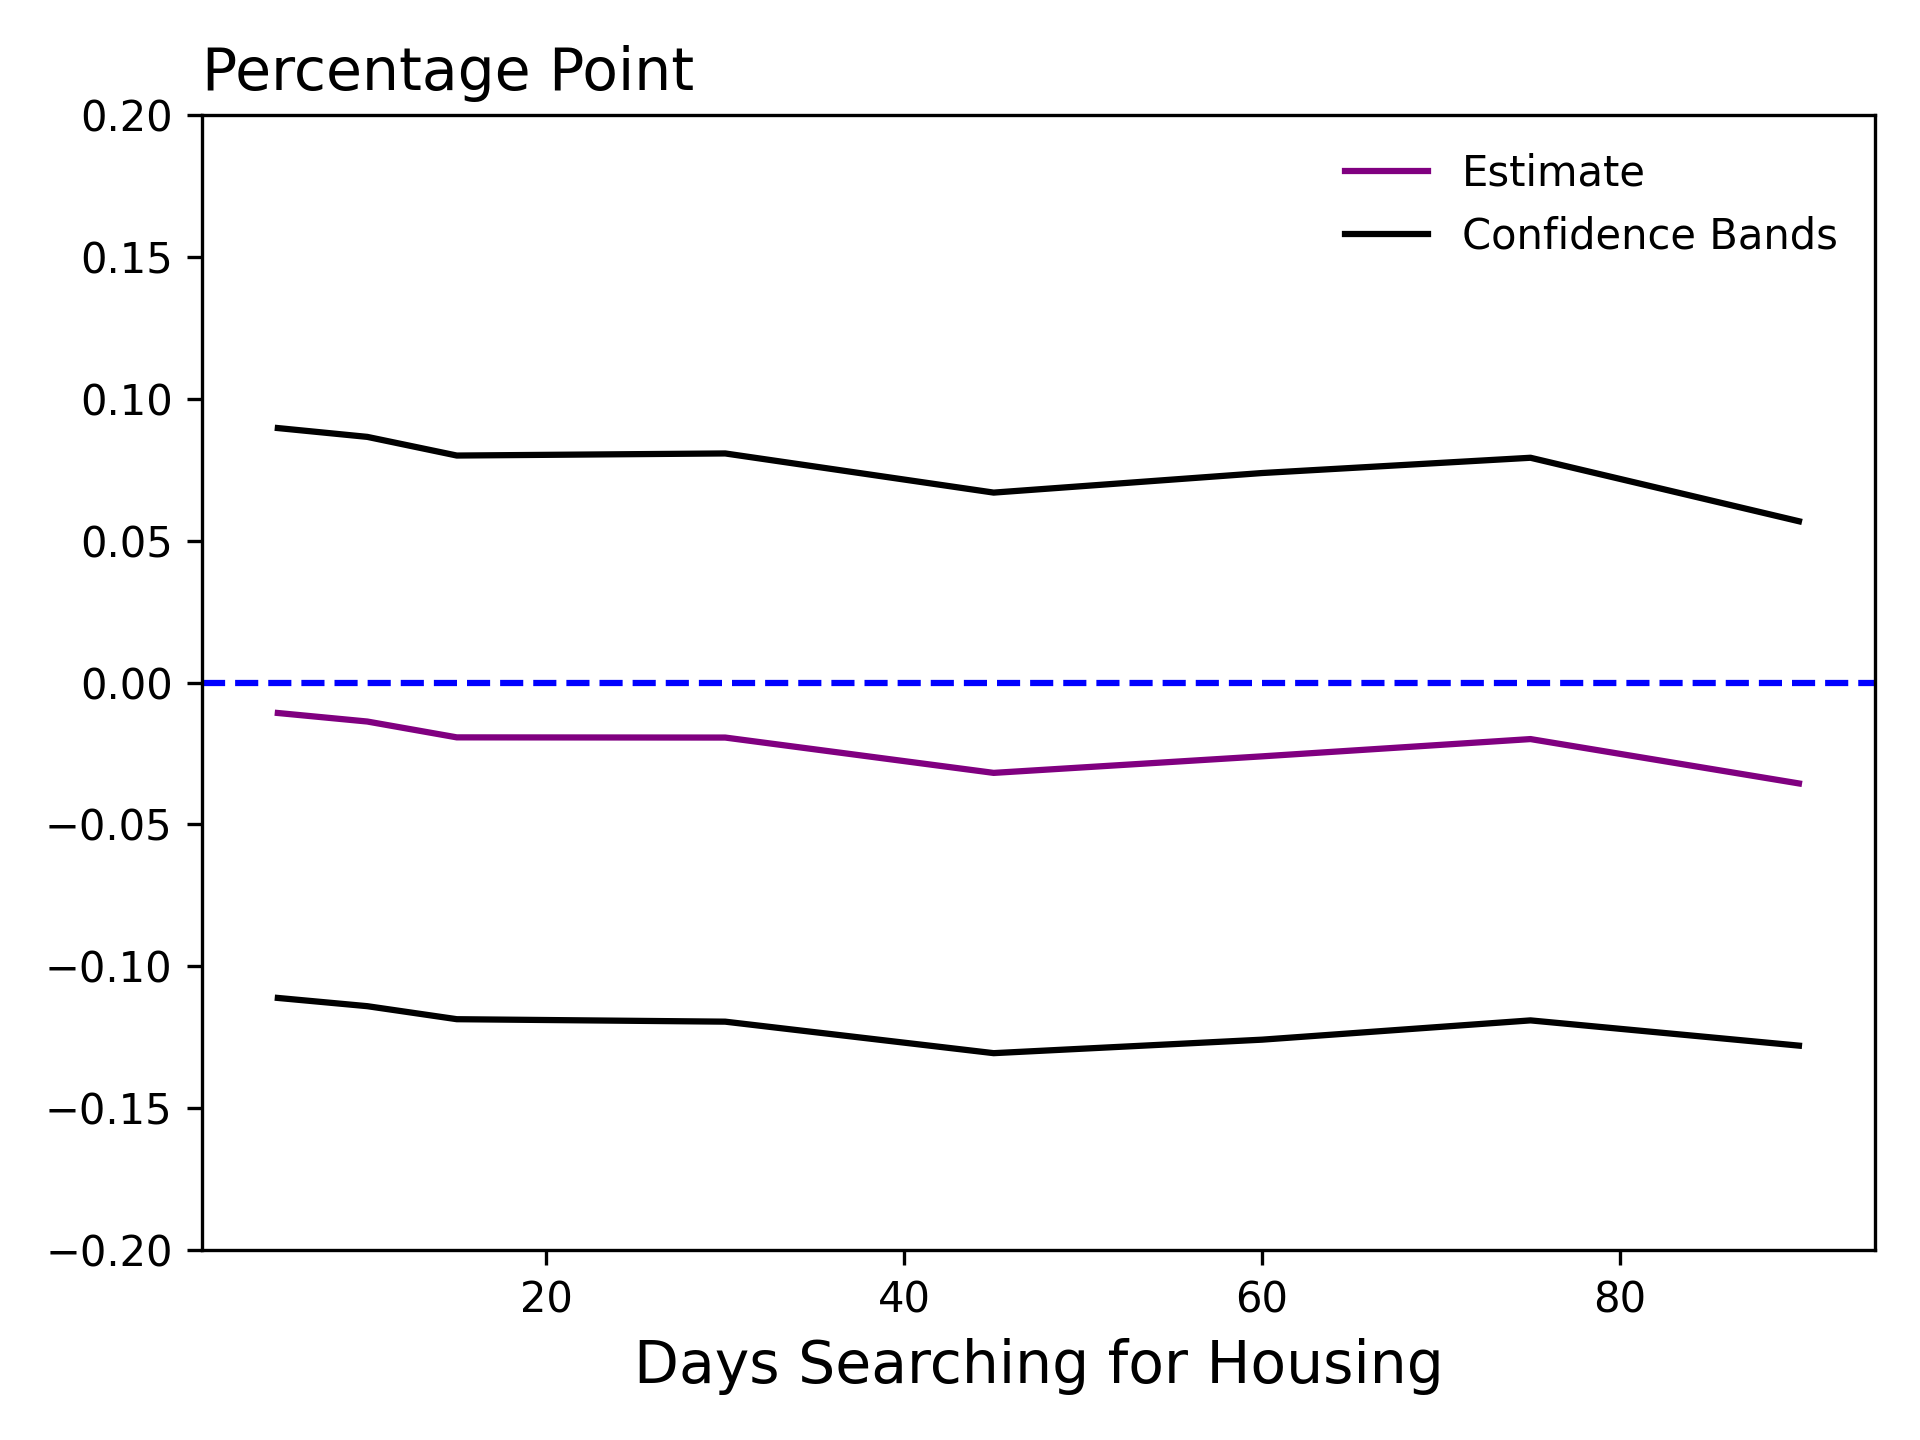
\includegraphics[width=.95\linewidth]{figures/rtc/results/cceh/rfp_False_False.png}
    \caption{All zip codes}
    \label{SUBFIGURE LABEL 3}
\end{subfigure}
\begin{subfigure}{.48\textwidth}
    \centering
    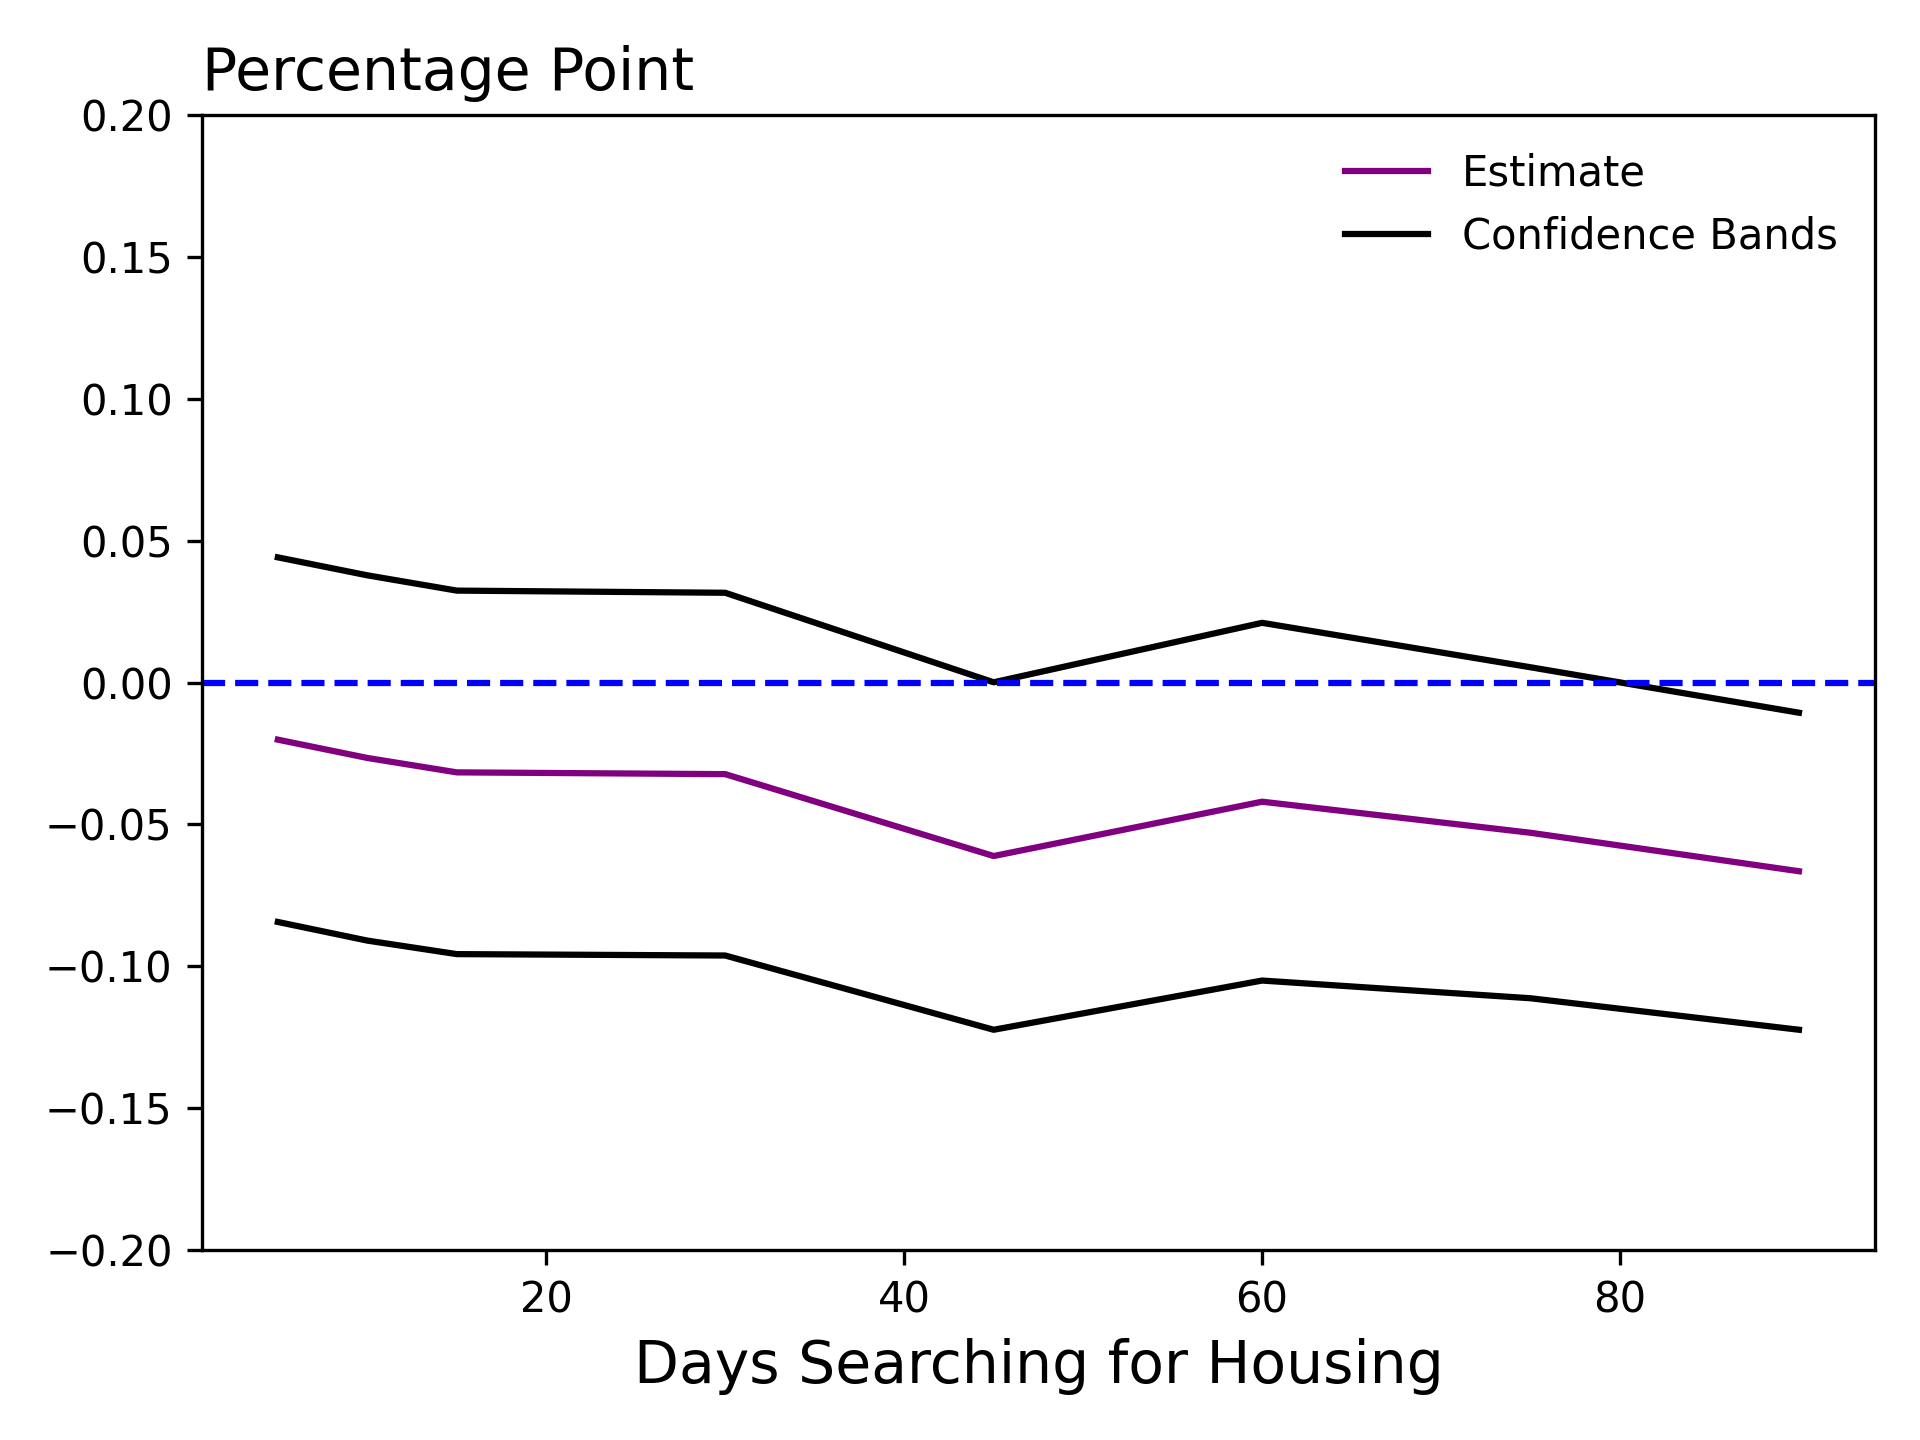
\includegraphics[width=.95\linewidth]{figures/rtc/results/cceh/rfp_True_False.png}
    \caption{High Eviction Zip Codes}
    \label{SUBFIGURE LABEL 4}
\end{subfigure}
\caption{ \href{https://github.com/pharringtonp19/evictions/blob/main/scripts/cceh/primary/cluster_diff_n_diff.py}{Reproduced Here}: Confidence Bands formed sampling across random parameter initializations}
\label{fig:rfp_results}
\end{figure}

\begin{figure}[htbp]
\centering
\begin{subfigure}{.48\textwidth}
    \centering
    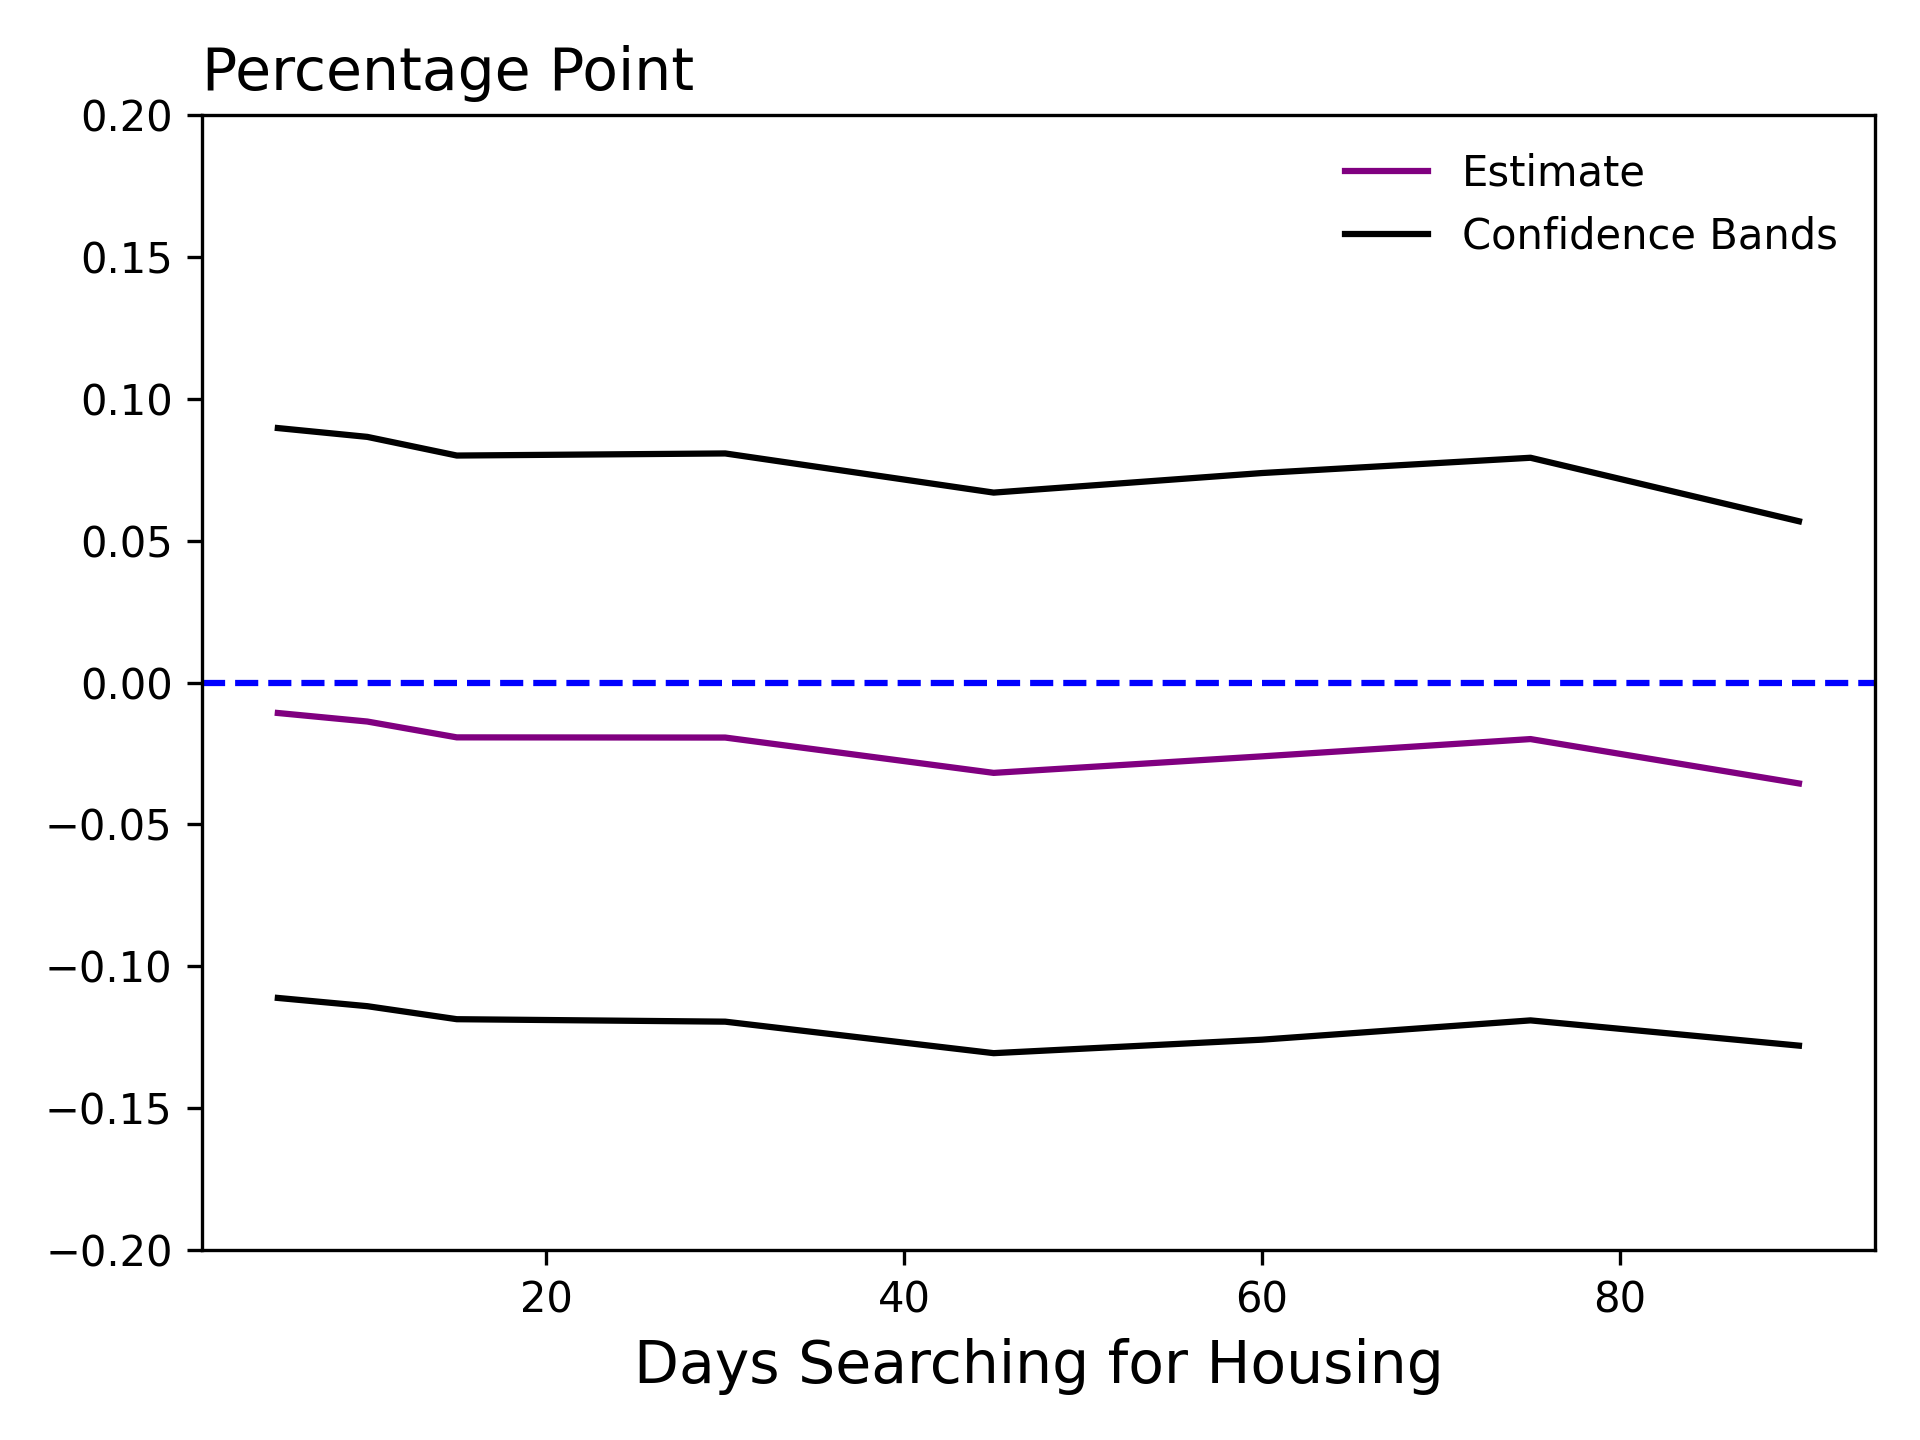
\includegraphics[width=.95\linewidth]{figures/rtc/results/cceh/rfp_False_False.png}
    \caption{All zip codes}
    \label{SUBFIGURE LABEL 3}
\end{subfigure}
\begin{subfigure}{.48\textwidth}
    \centering
    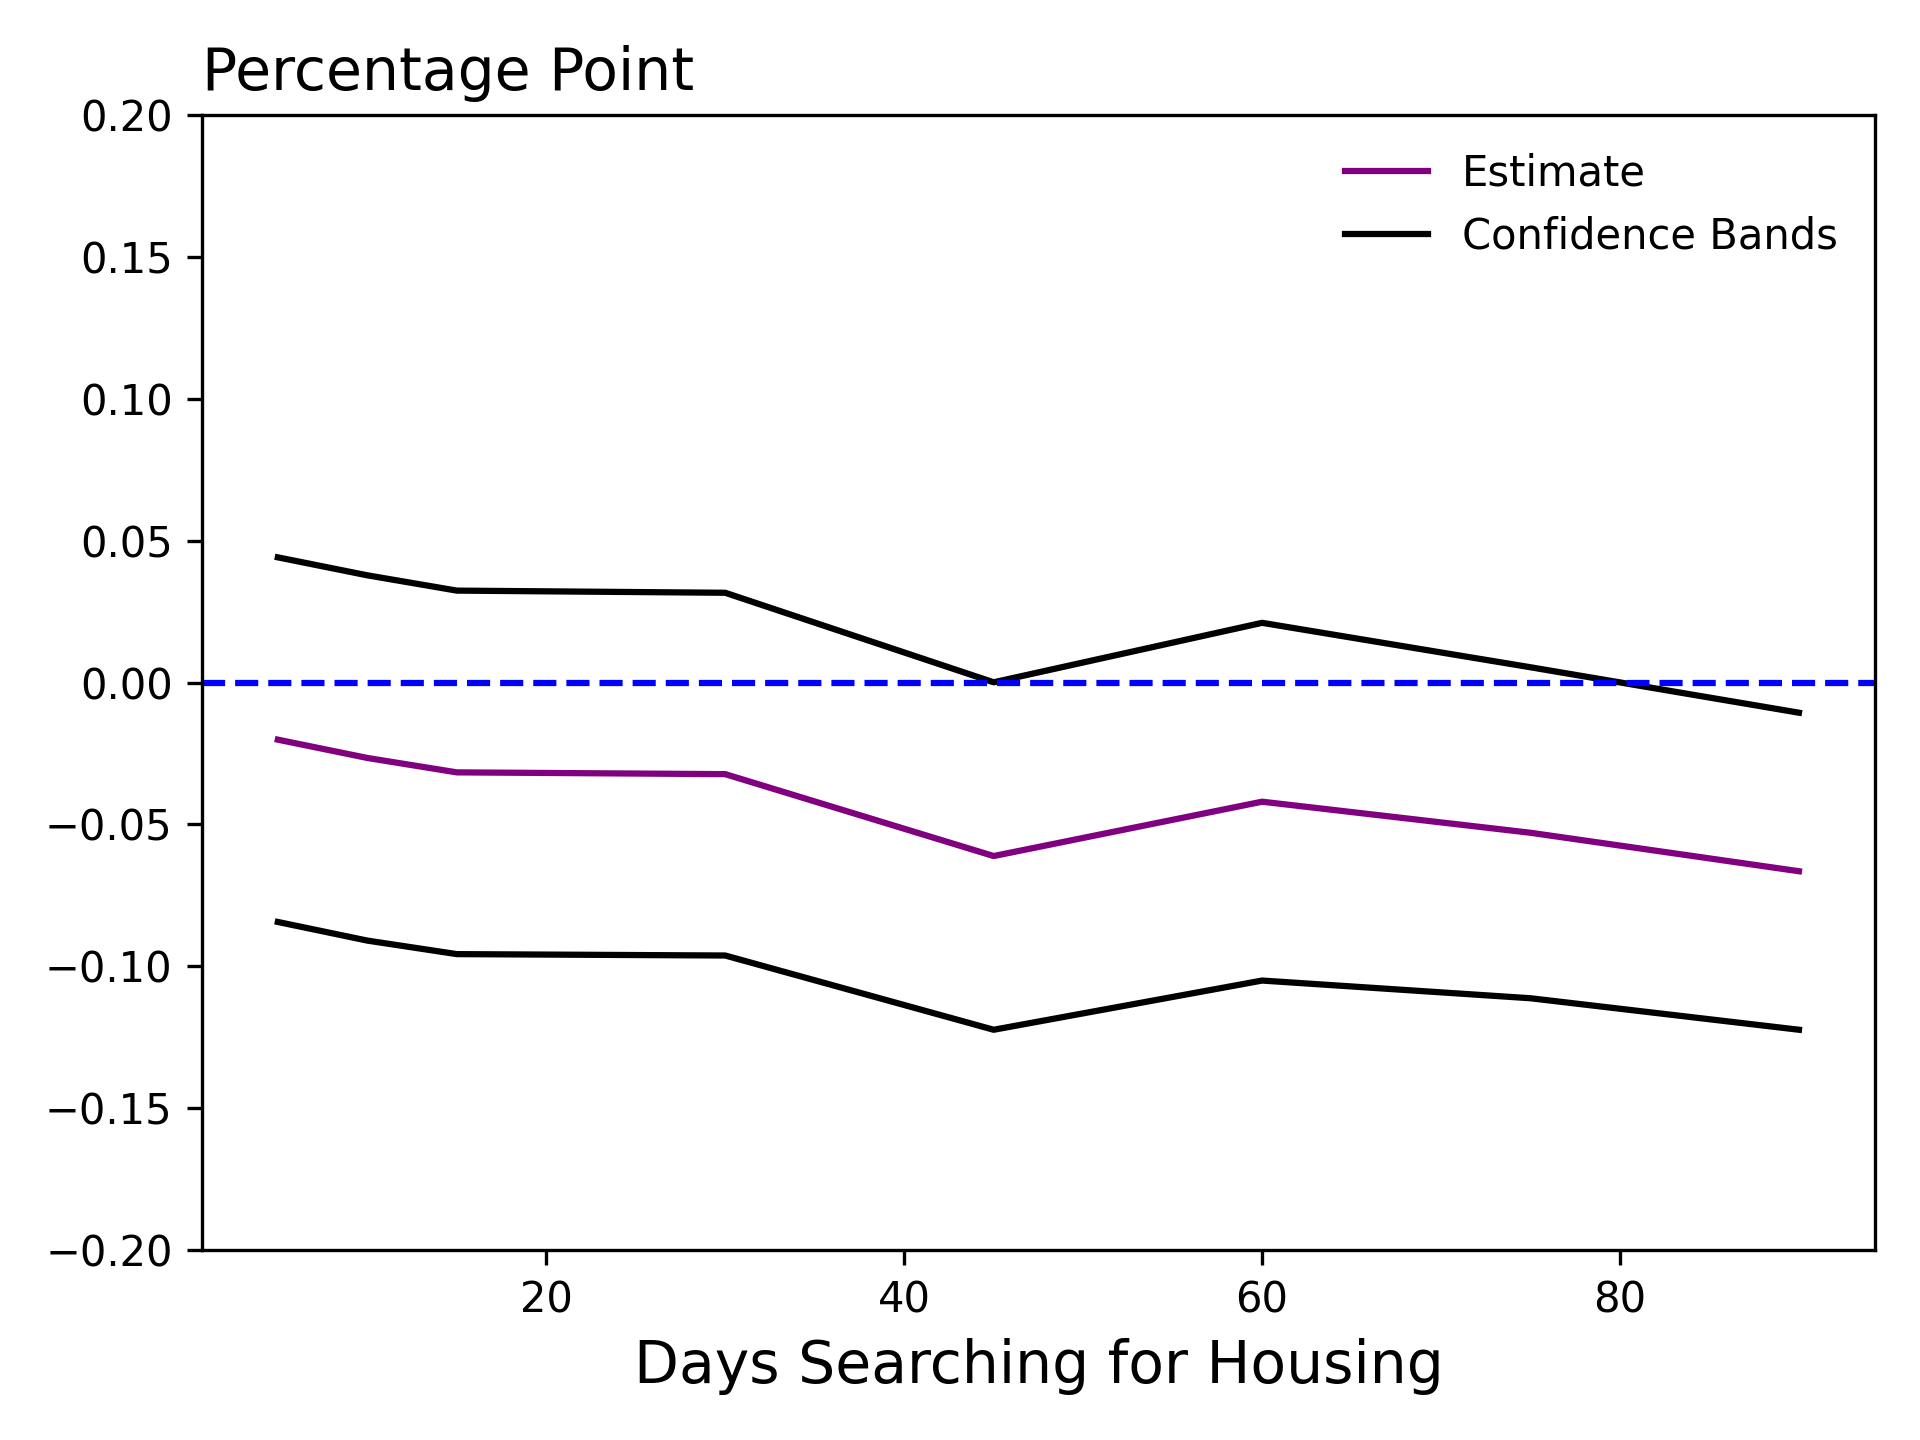
\includegraphics[width=.95\linewidth]{figures/rtc/results/cceh/rfp_True_False.png}
    \caption{High Eviction Zip Codes}
    \label{SUBFIGURE LABEL 4}
\end{subfigure}
\caption{ \href{https://github.com/pharringtonp19/evictions/blob/main/scripts/cceh/primary/cluster_diff_n_diff.py}{Reproduced Here}: Confidence Bands formed sampling across random parameter initializations}
\label{fig:rfp_results}
\end{figure}
While the magnitude of the effect shrinks, the sign of the effect is relatively constant and negative when restricting the sample to high eviction zip codes. We also note that the difference in the estimated effects when considering the all zip codes and only high eviction zip codes decrease. \par 
Over a long time frame, it would be interesting to assess whether the tail of the distribution increased. As \cite{evans2019reducing} notes in summaring previous homelessness related work, the costs are often associated with those in the tail.\footnote{\cite{evans2019reducing} notes that In Spellman et al. (2010), the costliest 10 percent of people incur up to 83 percent of the total costs of shelter
during homelessness. In Flaming et al. (2015), individuals with costs in the top 5 percent of the public costs
incur 47 percent of all costs. Hence, whether a program targets the costliest cases matters significantly for the
mean costs reported above.''}



\begin{align*}
    \tilde{Y}_i - \mathbb{E}[\tilde{Y}_i | X_i] &= \beta_0 (D_i - \mathbb{E}[D_i | X_i]) + v_i, \quad \tilde{Y}_i = Y_i - \mathbb{E}_{\textrm{pre}}[Y_i|X_i, Z_i] \\
\intertext{Extending the regression model in a nonparametric way is straightforward: simply integrate the transformed outcome across the features/covariates within each treatment group and take the difference. Presented in this way, it's clear that this approach only corrects for the presence of clustered data by using pre-treatment information and leaves to the post-treatment information on the table. Our framework can leverage both sources of information. While we leave a technical description of the framework to section \ref{sec:framework} of the paper}
\beta_0 &:= \int \mathbb{E}[ \tilde{Y}_i | X_i, D_i=1] - \mathbb{E}[ \tilde{Y}_i | X_i, D_i=0] d\mathbb{P}_X \\ 
\end{align*}
 
\section{Conclusion}
\begin{itemize}
    \item \href{https://nlihc.org/sites/default/files/Overview-of-National-Eviction-Moratorium.pdf}{Reference} Additional renter protections, such as right to counsel, expungement of eviction records, and just-cause
eviction standards, are needed to help protect renters now and in the long term.
\end{itemize}
The recent events of Covid-19 and rising inflation have magnified the importance and fragility of housing for low-income individuals. Indeed homelessness itself has become a staple in the news and political conversations (\href{https://www.nytimes.com/2022/10/31/opinion/oregon-governor-race.html}{NyTimes}). In response to this, we empirically assess the effectiveness of an initiative, growing in popularity across the U.S., known as the Right to Counsel (RTC). Currently adopted in 15 cities and 3 states, the initiative aims to combat the 3.6 million eviction fillings that occur each year in the U.S. by closing the gap in legal representation between landlord and tenant. Closing such a gap entails providing legal representation for tenants which as the case of Boston in 2019 which saw 39,594 eviction cases filed only  with only $8.7\%$ of tenants represented.\footnote{(\href{https://bostonbar.org/app/uploads/2022/06/rtc-report-for-web-or-email.pdf}{Samuelson et a. [2020]})}
Lastly, while no pre-analysis plan accompanies this paper, the only source of heterogeneity explored is the effects of the policy on Black and female tenants. As well documented in the eviction literature, these subgroups share the greatest likelihood and costs of evictions, as \cite{desmond2019unaffordable} writes, ``Low-income women, especially poor black women, are at high risk of eviction'', and \cite{collinson2022eviction} notes that with regards to the costs of evictions, ``We find particularly sharp negative impacts for female and Black tenants,\footnote{\cite{evans2019reducing} writes `} who drive the effects on labor market outcomes, residential mobility, and interactions with homelessness.'' It seems likely, therefore, that if landlords respond in an adverse way to The Right to Counsel, it would be be towards this sub-population in particular. Hence, all regression specifications are fit both over the entire sample and this sub-sample of interest. 
As a general statement, Economists are interested in understanding the effects of policies at scale. Almost by definition, though, these effects are not well identified. The aim, therefore, is to capture a particular effect of the policy as it's in the process of being deployed with the hope that this intermediate measurement might be informative about the effect under the new equilibrium.\par 
In this paper, we take as our intermediate measurement the housing search length for low-income individuals. As explained in the body of the paper, this is a far from perfect or comprehensive outcomes variable. That said, we regard as a meaningful signal in the sense that if there are adverse effects of the policy -- if landlords decide to re-optimize in an adverse fashion in response to the Right to Counsel -- we would likely see it via the housing search channel. \par 
And indeed, while extremely preliminary, we see some indication that there may be adverse effects along this channel. Across a series of estimators, each of which fits within a general empirical estimation structure of ``Regularizing the Forward Pass'' which we introduce in this paper, we see that search length increases.

%\bibliographystyle{plainnat}
\bibliography{bibliography.bib}

\section{Appendix}

\subsection{Regularized ODE}
\begin{align*}
    \textrm{prox}_{\lambda, f}(v) := \underset{x}{\textrm{argmin}} \ \Big( f(x) + \frac{1}{2\lambda} \| x - v \|^2\Big)
\end{align*}
\begin{figure}[htbp]
\centering
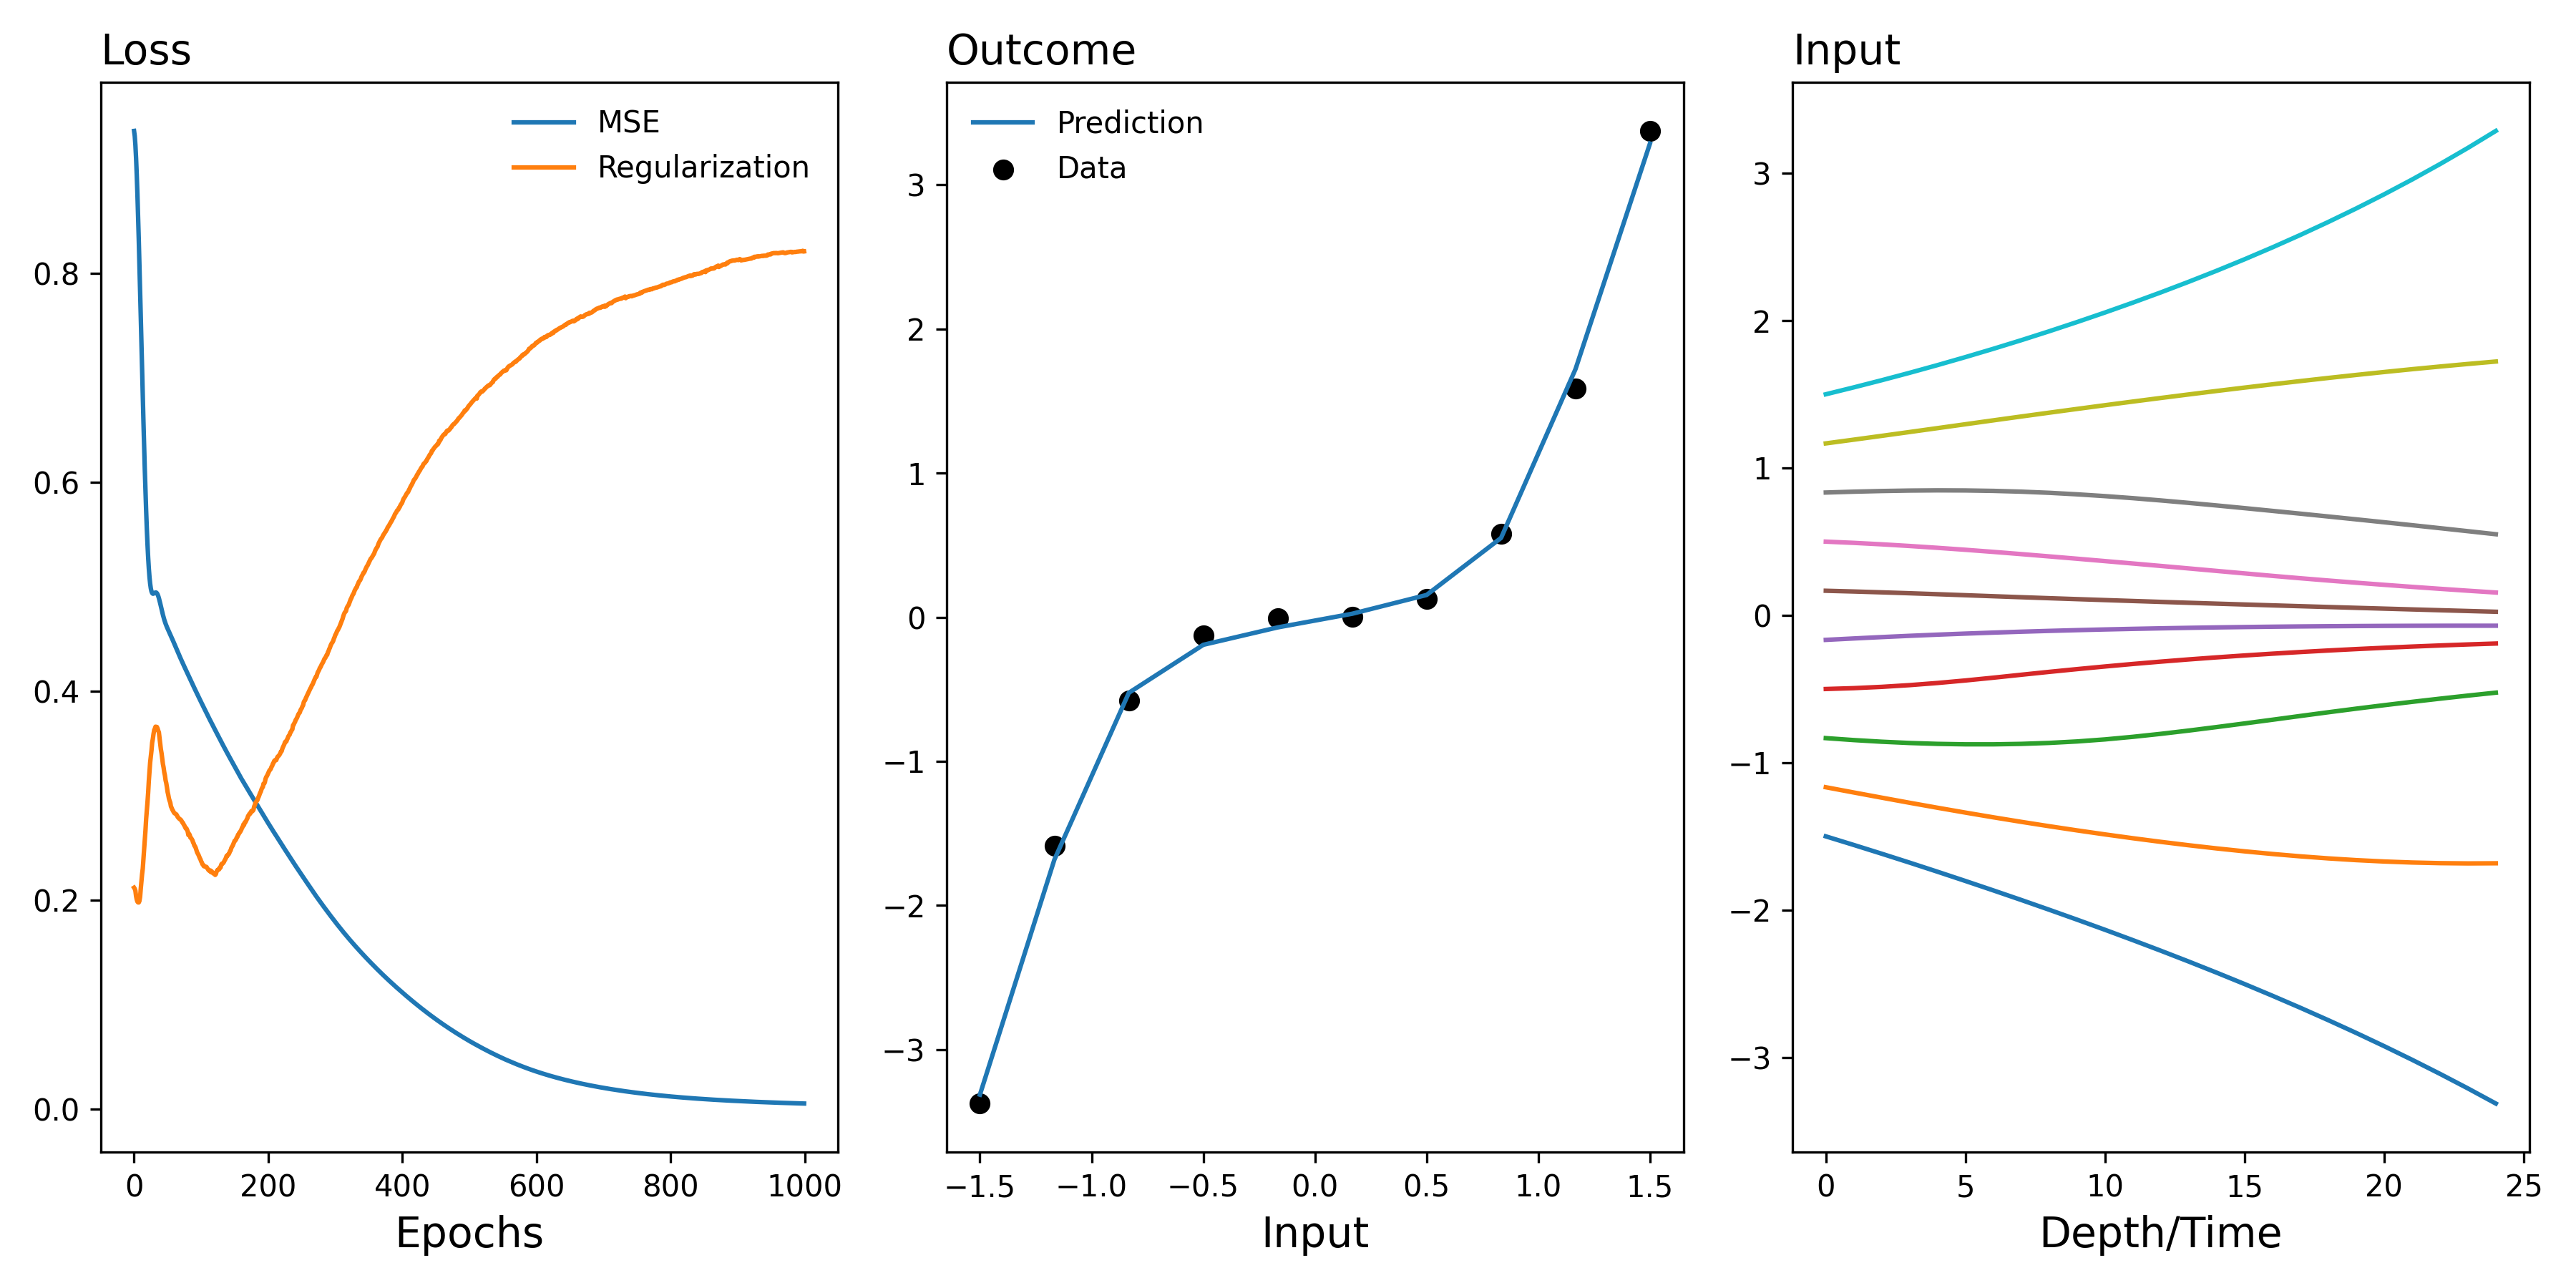
\includegraphics[width=0.8\textwidth]{figures/framework/reg_ode_0.0.png}
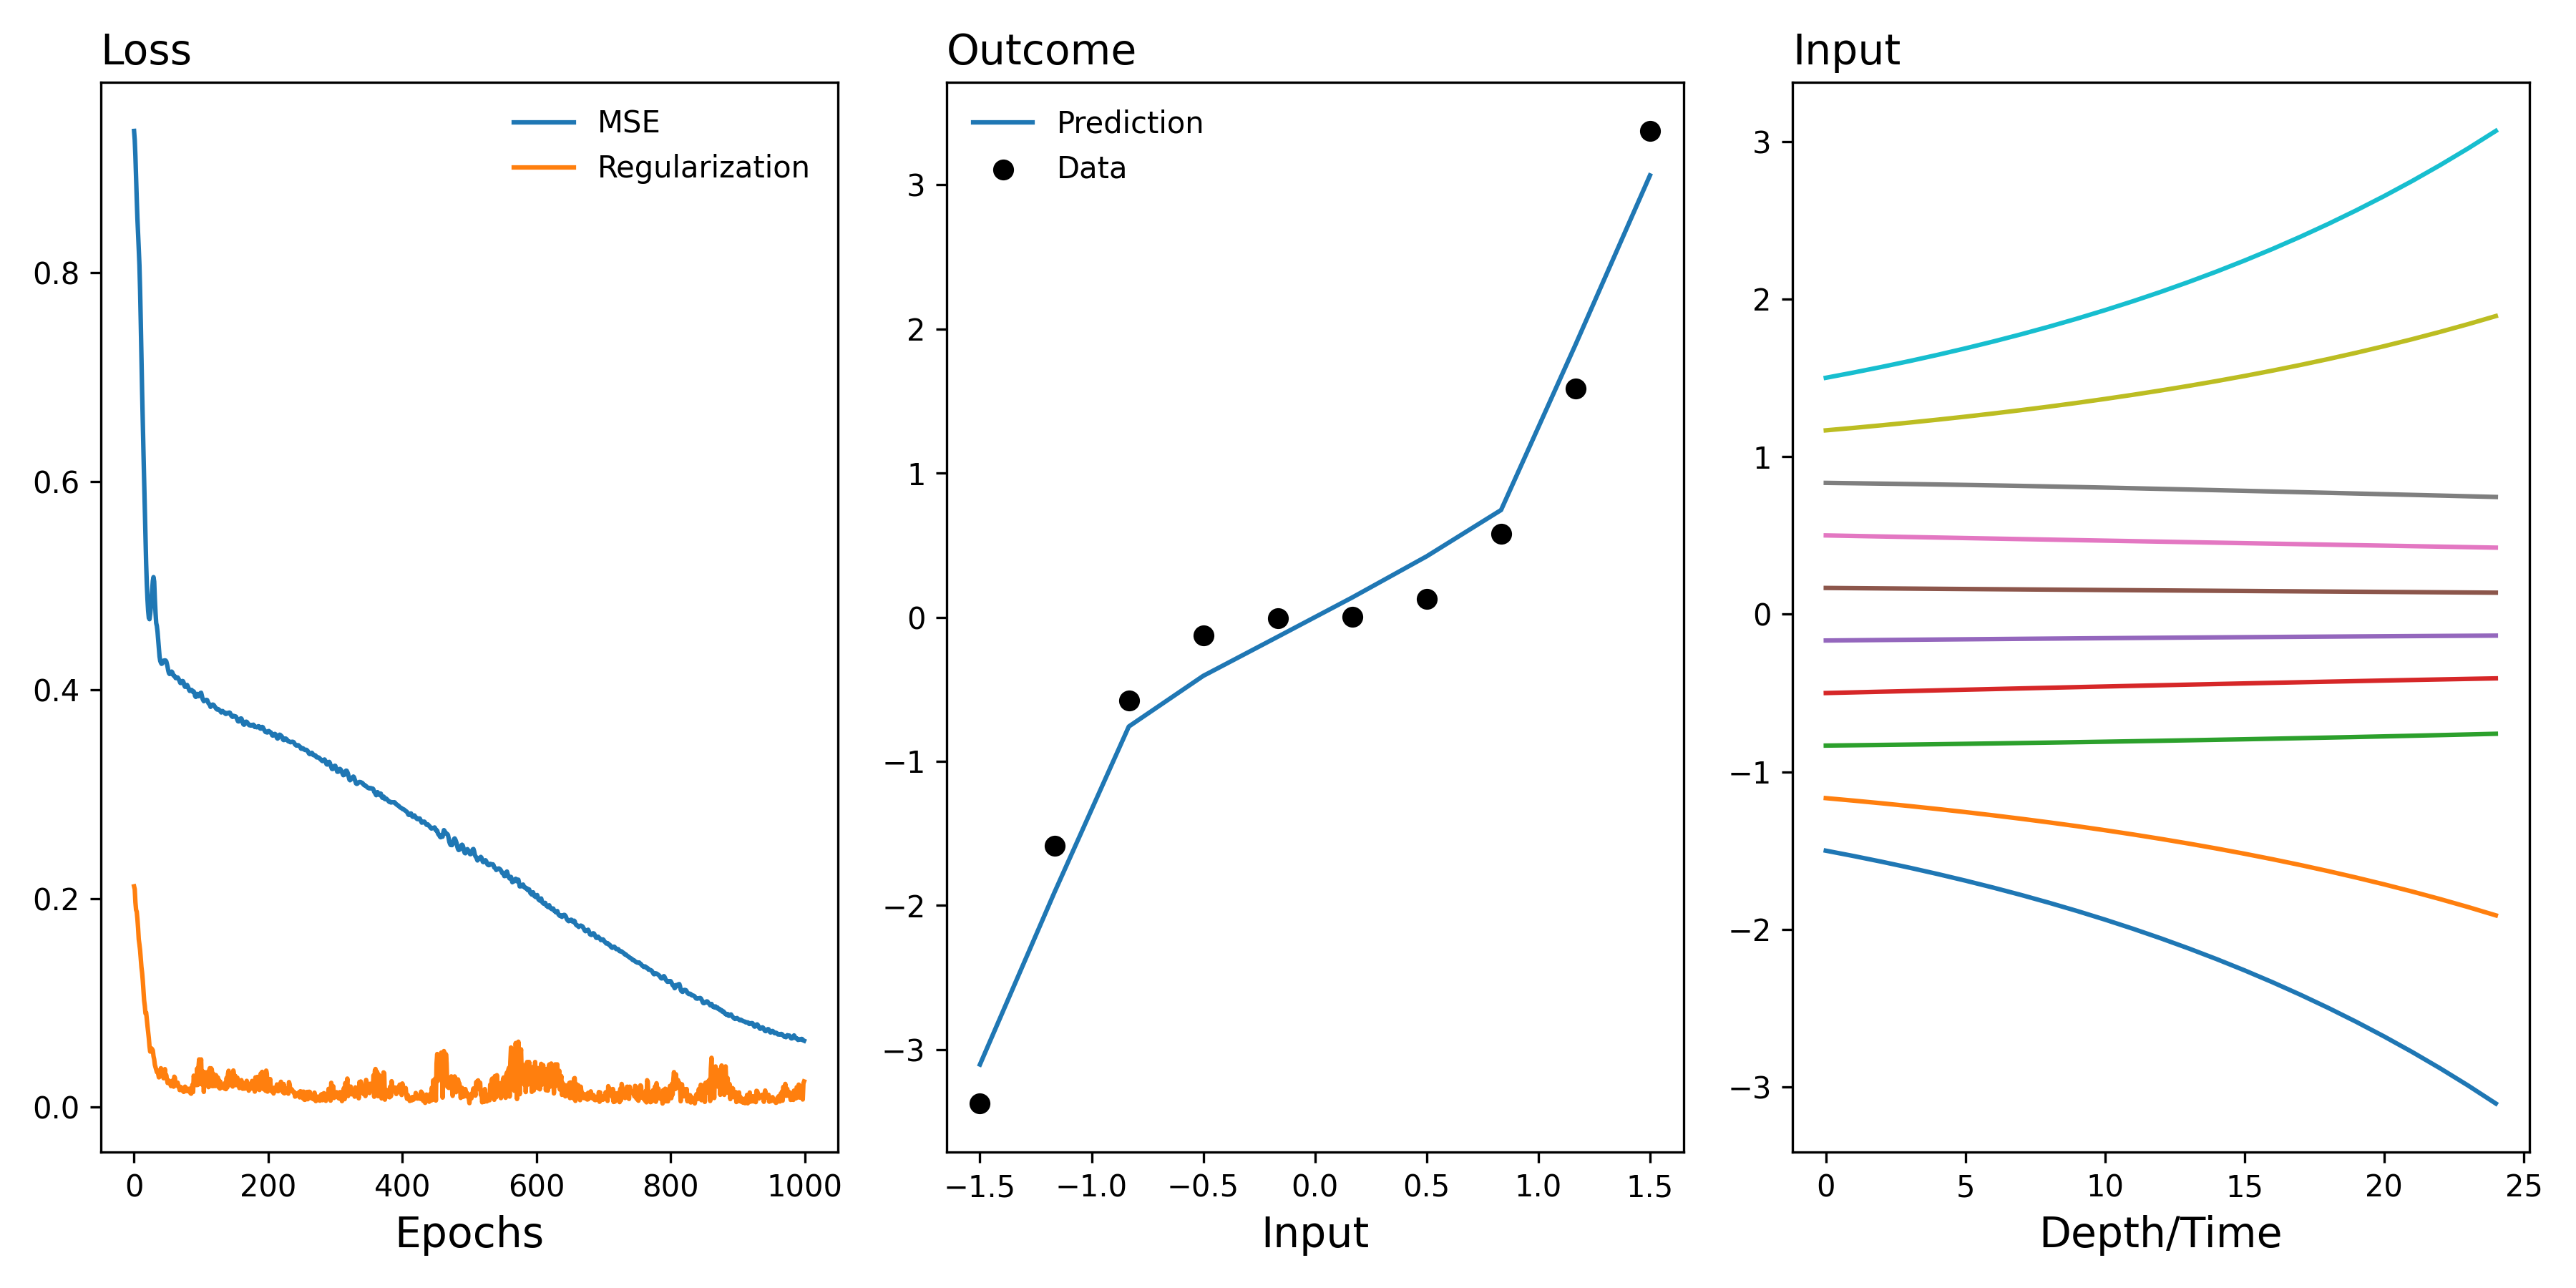
\includegraphics[width=0.8\textwidth]{figures/framework/reg_ode_10.0.png}
        \caption{High Level Summary}
        \label{fig:hls}
\end{figure}

\subsection{Inductive Bias}
\label{subsec:ib}


\begin{figure}[htbp]
\centering
\begin{subfigure}{.32\textwidth}
    \centering
    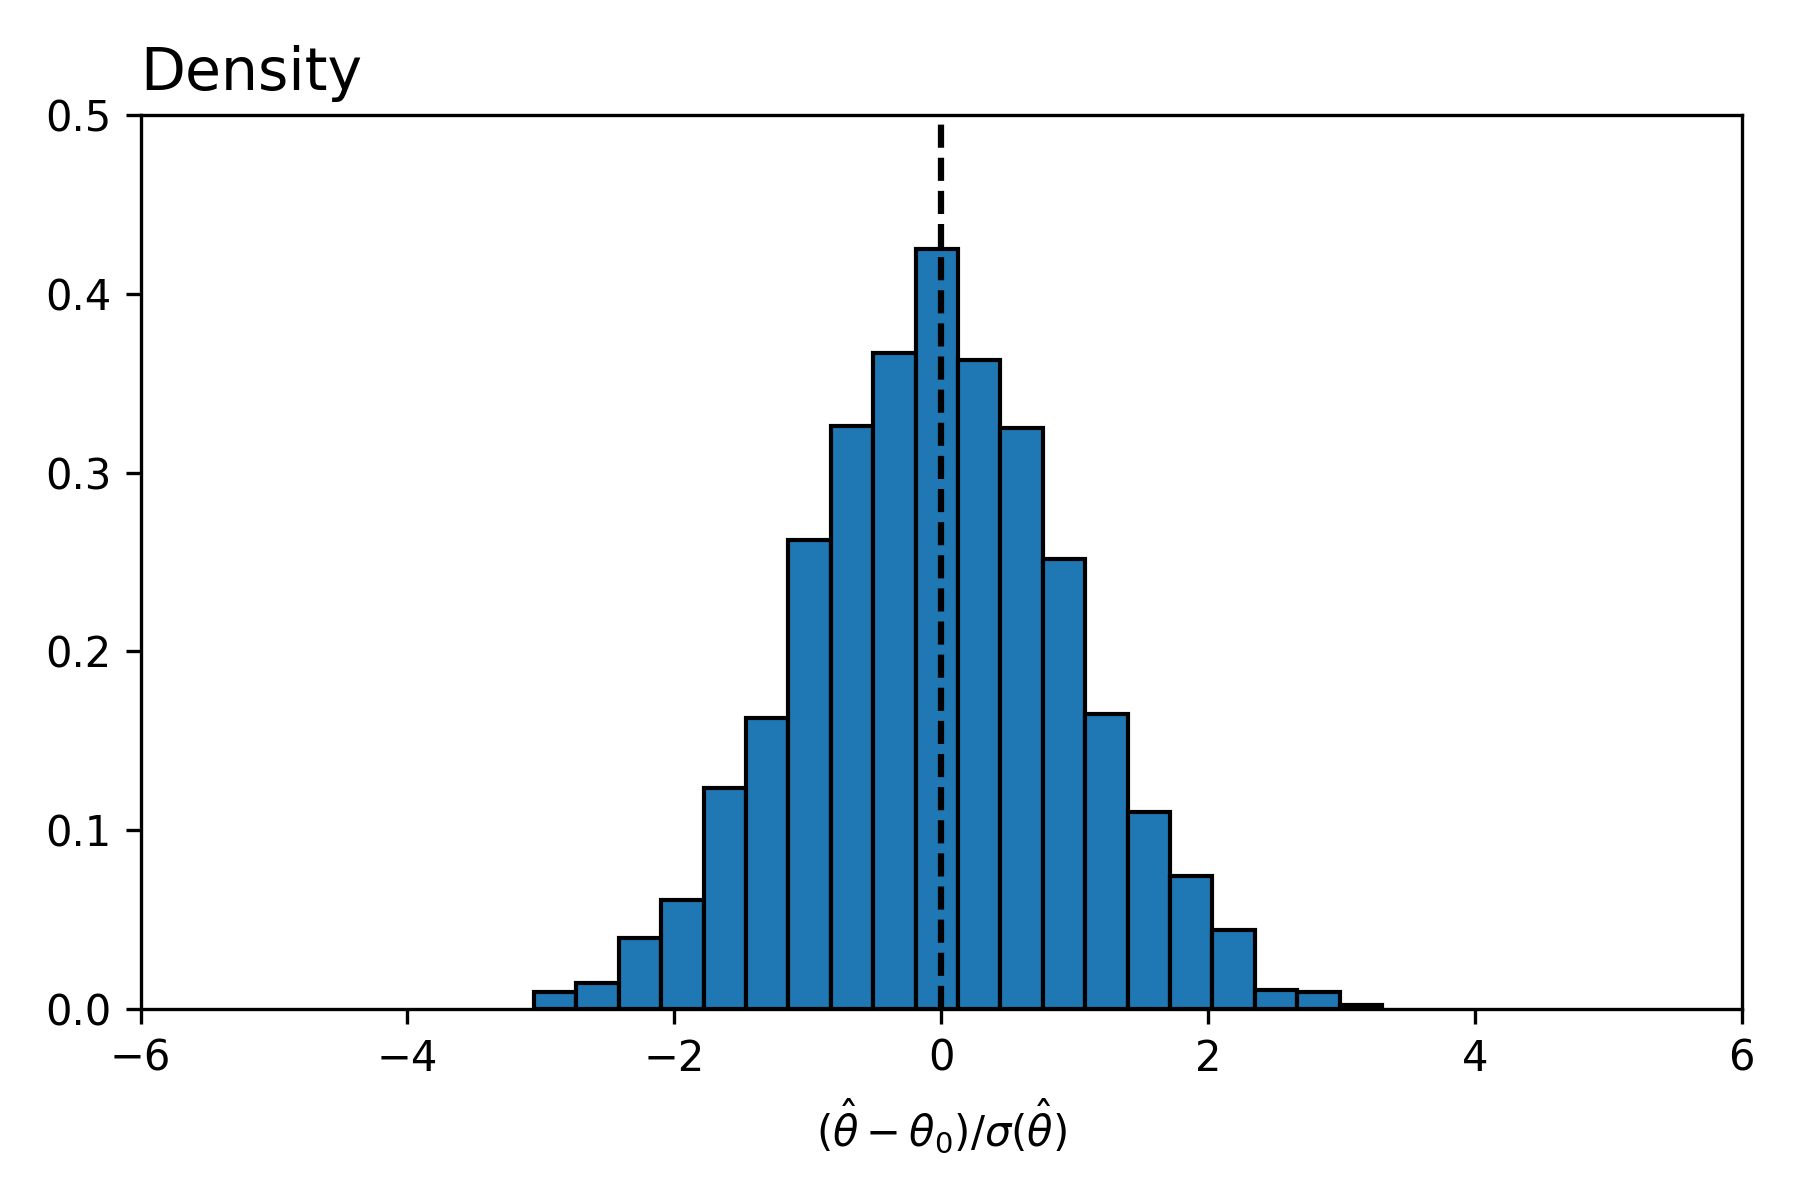
\includegraphics[width=.95\linewidth]{figures/framework/dml_original.png}
    \caption{Double Machine Learning}
    \label{fig:overfittails}
\end{subfigure}
\begin{subfigure}{.32\textwidth}
    \centering
    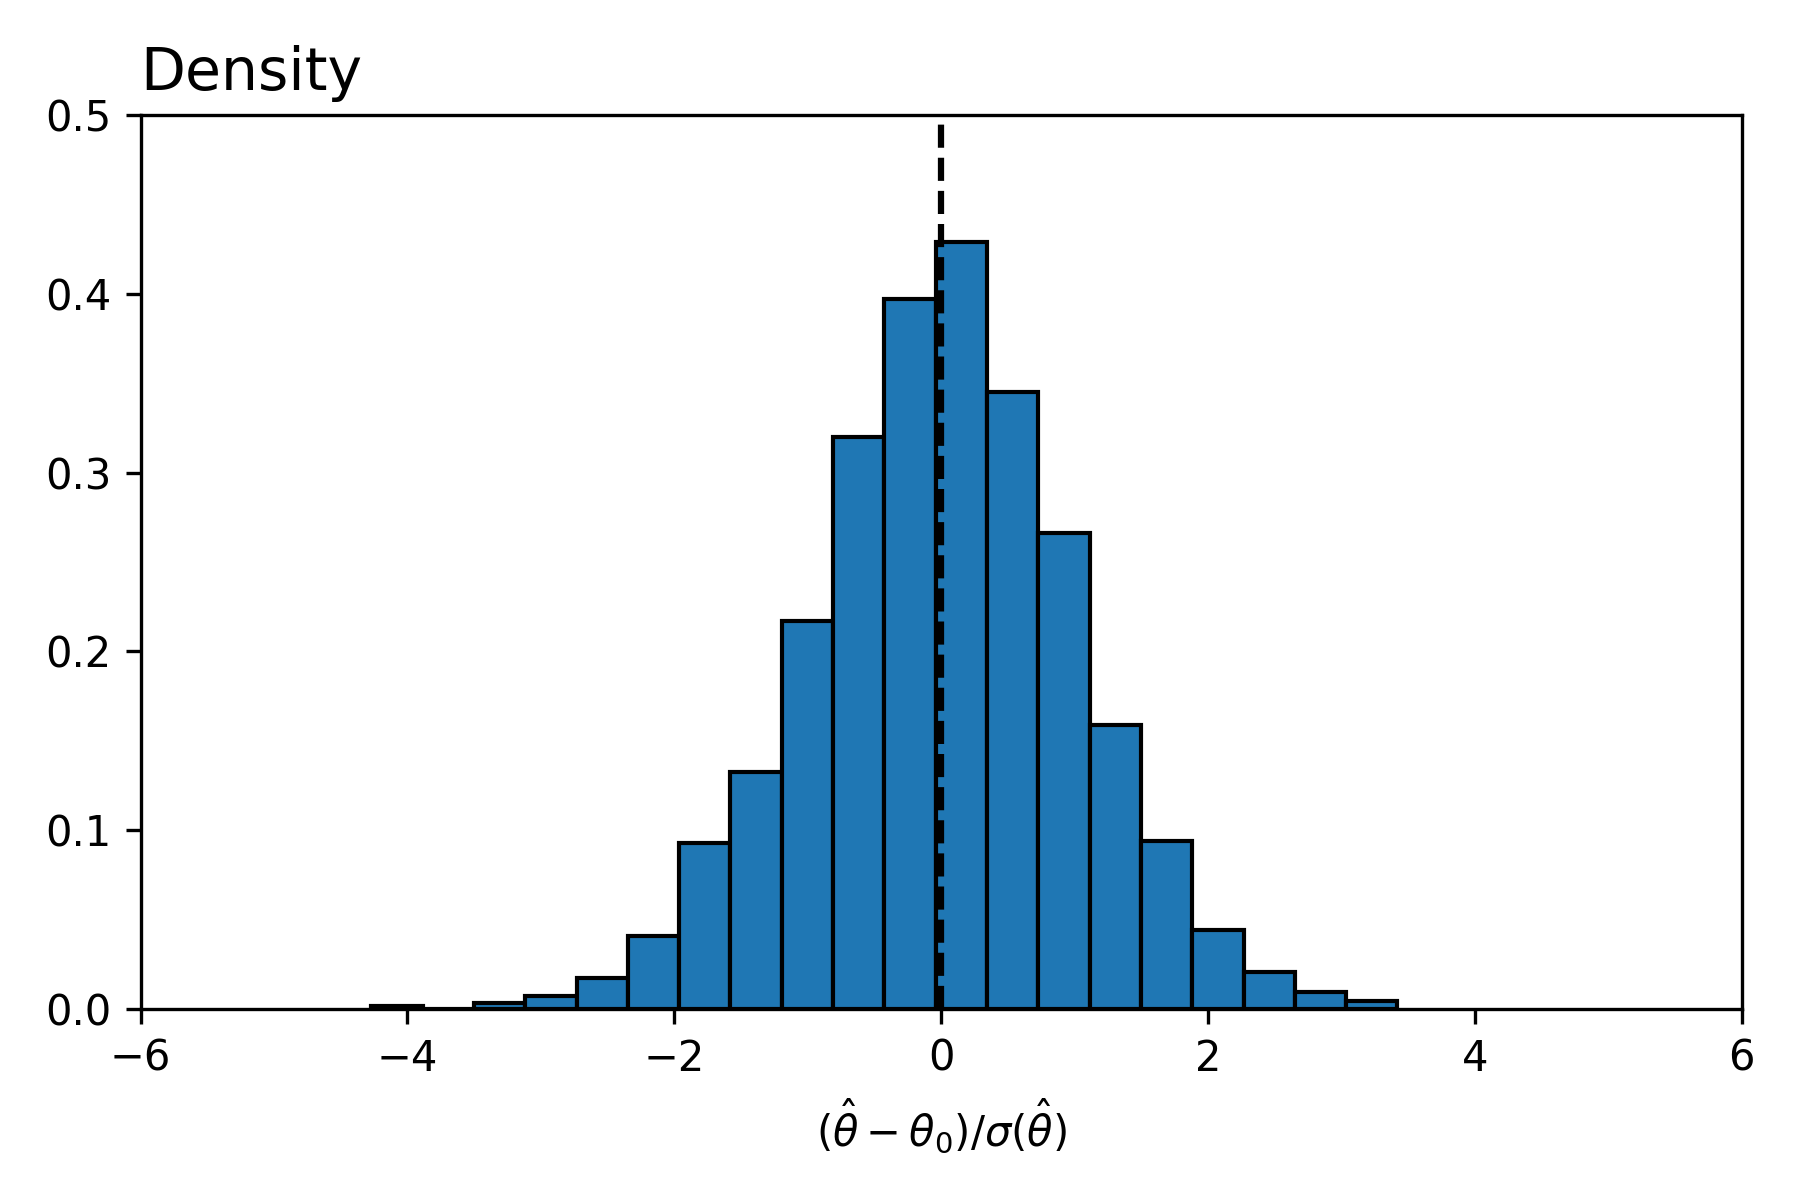
\includegraphics[width=.95\linewidth]{figures/framework/dml_standard_nn.png}
        \caption{Standard Deep Learning}
    \label{fig:wrongspace}
\end{subfigure}
\begin{subfigure}{.32\textwidth}
    \centering
    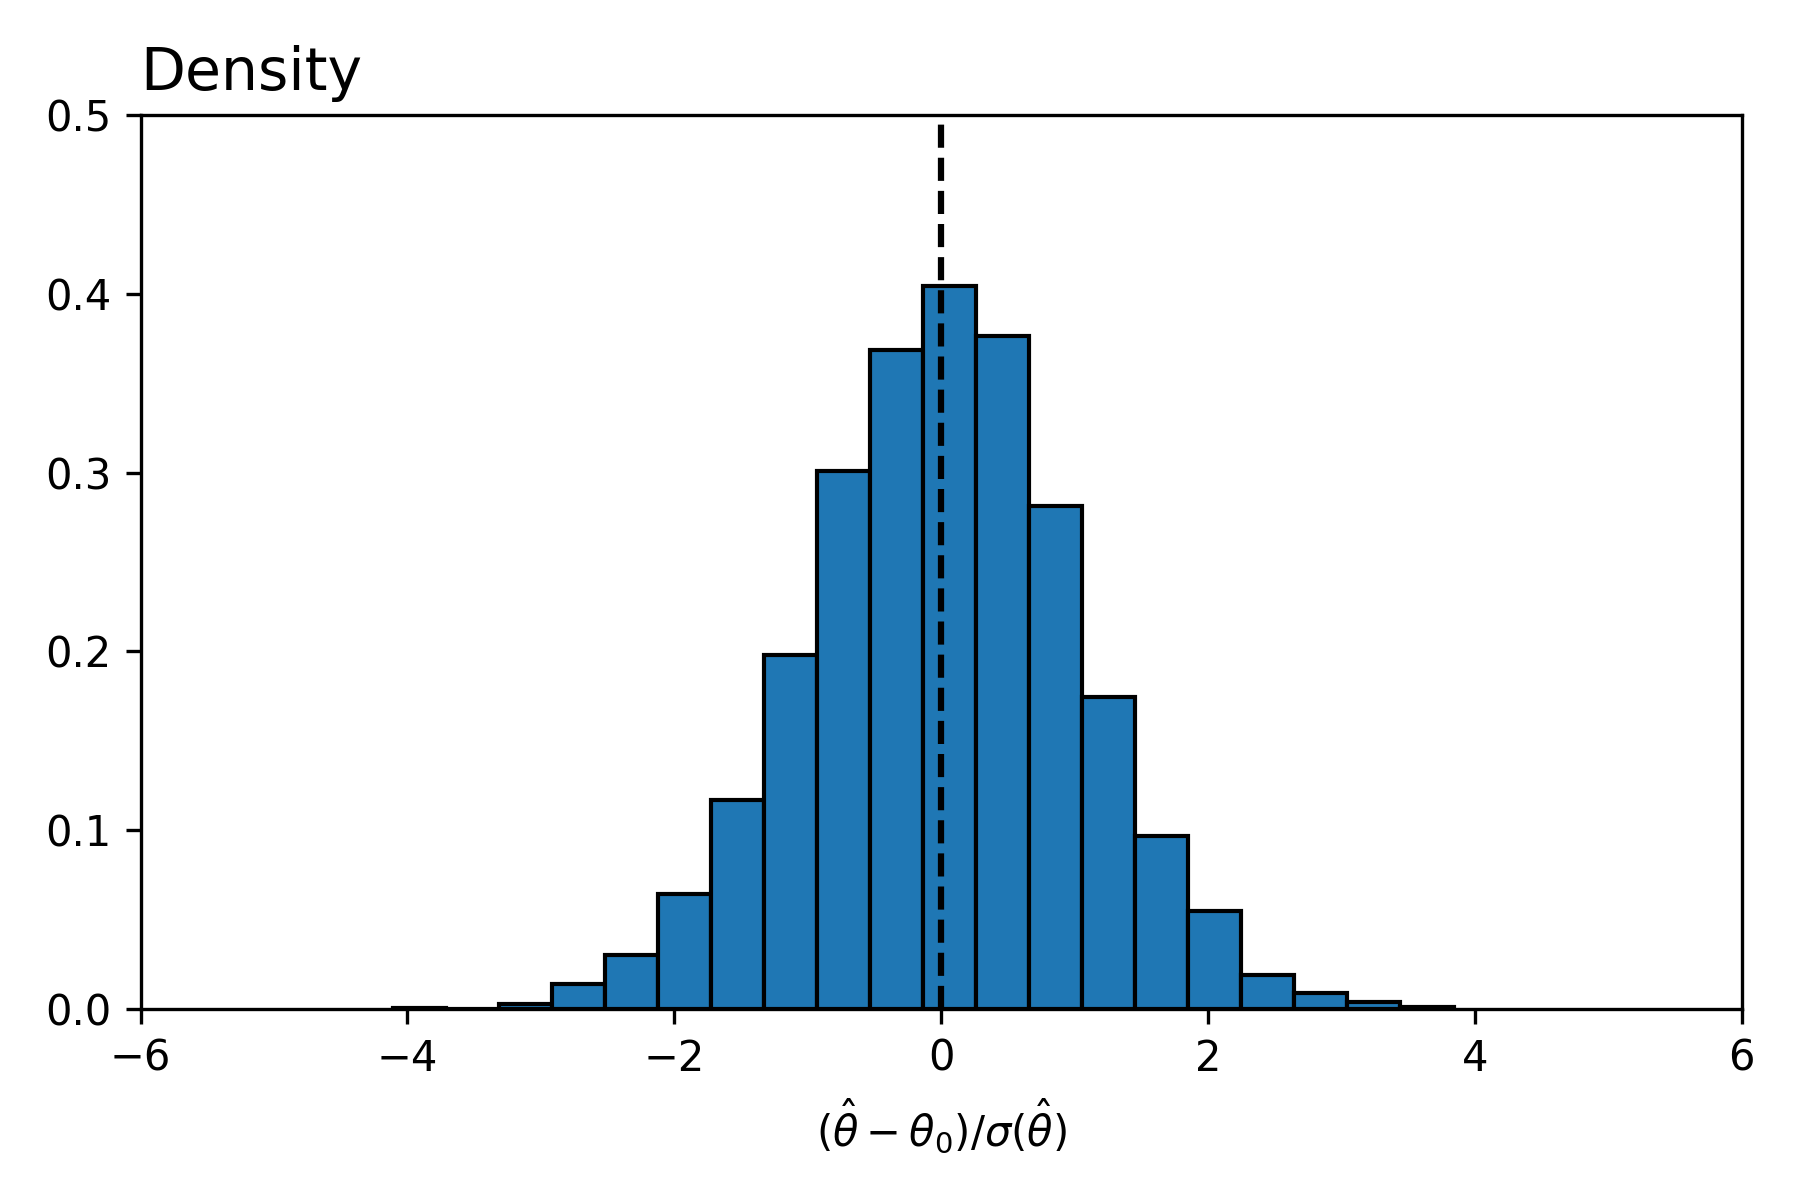
\includegraphics[width=.95\linewidth]{figures/framework/dml_linear_comp.png}
        \caption{Linear Regression}
    \label{fig:rfp}
\end{subfigure}
\caption{ \href{https://github.com/pharringtonp19/rfp/blob/main/notebooks/grad_desc_toy.ipynb}{Reproduced Here}: The grey and black dots represent data from separate clusters. Each figure corresponds to fitting a neural network to this data under different training algorithms}
\label{fig:mamlablation}
\end{figure}

\subsection{Implementation Details}
\begin{itemize}
    \item (\href{https://www.cga.ct.gov/2021/ACT/PA/PDF/2021PA-00034-R00HB-06531-PA.PDF}{"Income-eligible"} means (A) having household income at or below
eighty per cent of the state median income adjusted for family size, as
determined by the United States Department of Housing and Urban
Development, at the time of the request for representation; or (B)
receiving one of the following types of public assistance: (i) Temporary
Assistance for Needy Families, (ii) Supplemental Nutrition Assistance
Program benefits, (iii) Medicaid, (iv) Supplemental Security Income, (v)
refugee resettlement benefits, (vi) rental assistance under chapter 138a
of the general statutes, or (vii) the federal Housing Choice Voucher
Program, 42 USC 1437f(o);
\end{itemize}
\subsection{Detailed Timeline}
\begin{itemize}
    \item \href{https://nlihc.org/sites/default/files/Overview-of-National-Eviction-Moratorium.pdf}{Reference}: The CDC eviction moratorium took effect September 4 and was initially set to expire on December 31.
Congress extended the moratorium through January 2021 – and President Biden further extended it
through March, June, and July – and provided a total of \$46.5 billion for emergency rental assistance
(ERA). The eviction moratorium lapsed on July 31, but the CDC announced on August 3 a limited eviction
moratorium through October 3 for renters living in communities experiencing a surge in COVID-19 cases,
covering an estimated 80% of all U.S. counties and 90% of all renters. The CDC’s announcement came one
day after the Biden administration announced additional steps it will take to protect renters and prevent
evictions during the pandemic, including those recommended by NLIHC and the National Housing Law
Project.
 
    \item \href{https://nlihc.org/sites/default/files/Overview-of-National-Eviction-Moratorium.pdf}{Reference} The Centers for Disease Control and Prevention (CDC) took unprecedented action on September 1 by
issuing a temporary national moratorium on most evictions for nonpayment of rent to help prevent
the spread of coronavirus. Citing the historic threat to public health posed by coronavirus, the CDC
declared that an eviction moratorium would help ensure people are able to practice social distancing
and comply with stay-at-home orders. The CDC issued on October 9 guidance creating new burdens
for renters seeking moratorium protections. While the new guidance does not rescind the moratorium
on most evictions for nonpayment of rent, it states that landlords may challenge tenant declarations and
initiate eviction proceedings at any time. The new guidance undermines the intent of the CDC’s order by
eroding protections for renters and making it more difficult for struggling renters to remain stably housed.
\item CDC argues coronavirus presents a historic threat to public health and eviction
moratoriums can be an effective public health measure to prevent the spread of coronavirus. An eviction
moratorium is necessary to ensure people are able to follow best practices recommended by the CDC to
cut down on coronavirus transmission, including quarantine, isolation, and social distancing. 
\item Evictions – even a single eviction filing – creates a longterm mark on a renter’s record, hindering their access to future housing opportunities.
\end{itemize}

\begin{comment}

\subsection{Context Plots}
\begin{figure}[htbp]
\centering
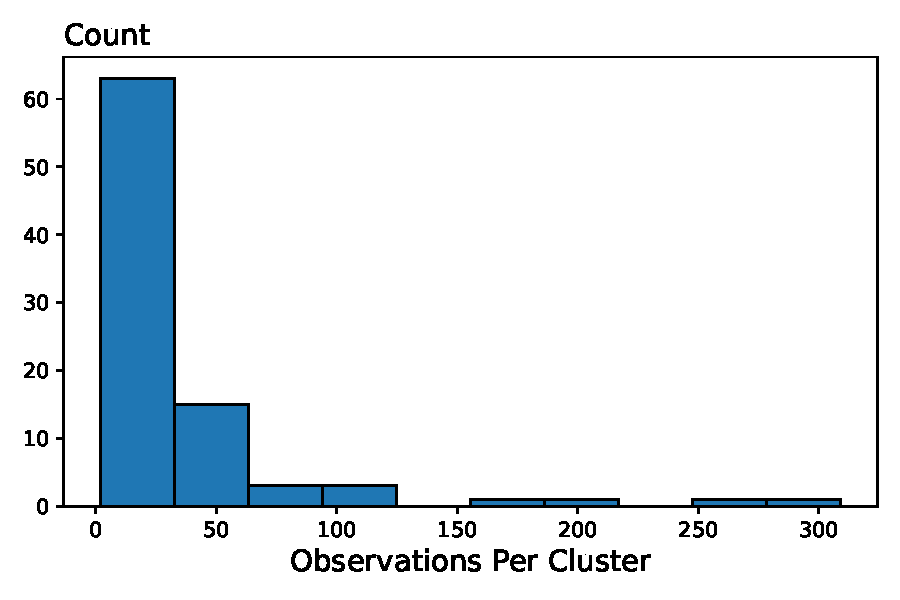
\includegraphics[width=.5\linewidth]{figures/rtc/results/cceh/cluster_dist_False_False.pdf}
\caption{ \href{https://github.com/pharringtonp19/evictions/blob/main/scripts/cceh/primary/diff_n_mean_rrh.py}{Reproduced Here}}
\label{FIGURE LABEL}
\end{figure}
\subsection{High-Level Overview of Model}
\begin{align*}
\intertext{Test}
    &l \circ f \circ c \\ 
\intertext{Training} 
    &l >=> f >=> c \\ 
\end{align*}

\subsection{Category Theory Explanation}
\begin{align*}
&\textrm{class Functor} \ f \ \textrm{where} \\ 
&\quad \textrm{fmap} \ :: \ (a \to b) \to (f \ a \to f \ b) \\ \\ 
&\textrm{instance Functor RFP where} \\ 
&\quad \textrm{fmap} \ f \ (x, r) = (f \ x, g(f) \ x + r)  \\ 
\end{align*}
\begin{quote}
    \textbf{Type Class}: It's not enough to simply restrict the number of iterations of the inner loop. You need to fmap! That is, fmap is regularizing the forward pass: a statistic you compute during the forward pass. To be exact, we're defining a specific functor which is captured in haskell via the implementation of fmap. 
\end{quote}
If we make the simplification that we have two types, Data and Params, then our neural networks models can be thought of as functions between these sets: the clusterMap maps from Params to Params and the featureMap from Params to Data. With this, we have a category. \par 
As explained in section \ref{sec:framework}, during training, we would like our neural network models to return a regularization value in addition to the predictions. We can do so with the help of a functor\footnote{As illustrated via the math, as programmers our functors can be thought of as a type constructor - \cite{milewski2019category}} which maps our category into a new category. For the types, it augments them the the regularization value. And for our neural network models, it embelleshes them so that they return both desired outputs. Just from this, it is then evident that when we are training the model, we are working in one category while during inference we're working in another.\par 
\begin{align*}
\intertext{Type Constructor}
&\textrm{data Reg a} = \textrm{Float} \  \& \ a \\ 
\intertext{fmap}
&\textrm{fmap} :: (a \to b) \to (\textrm{Reg a}  \to \textrm{Reg a} )
\end{align*}
This structure highlights that the key design choice is the fmap (how do you explicitly penalize the neural network).
\subsection{Framework Motivation}
\begin{figure}[htbp]
\centering
\begin{subfigure}{.48\textwidth}
    \centering
    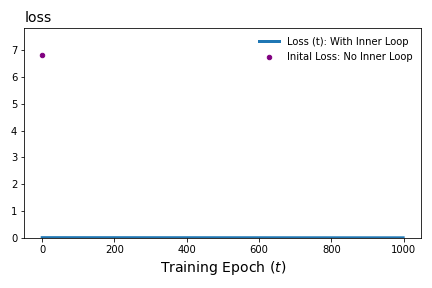
\includegraphics[width=.95\linewidth]{figures/framework/full_inner_loop.png}
    \caption{}
    %\label{SUBFIGURE LABEL 3}
\end{subfigure}
\begin{subfigure}{.48\textwidth}
    \centering
    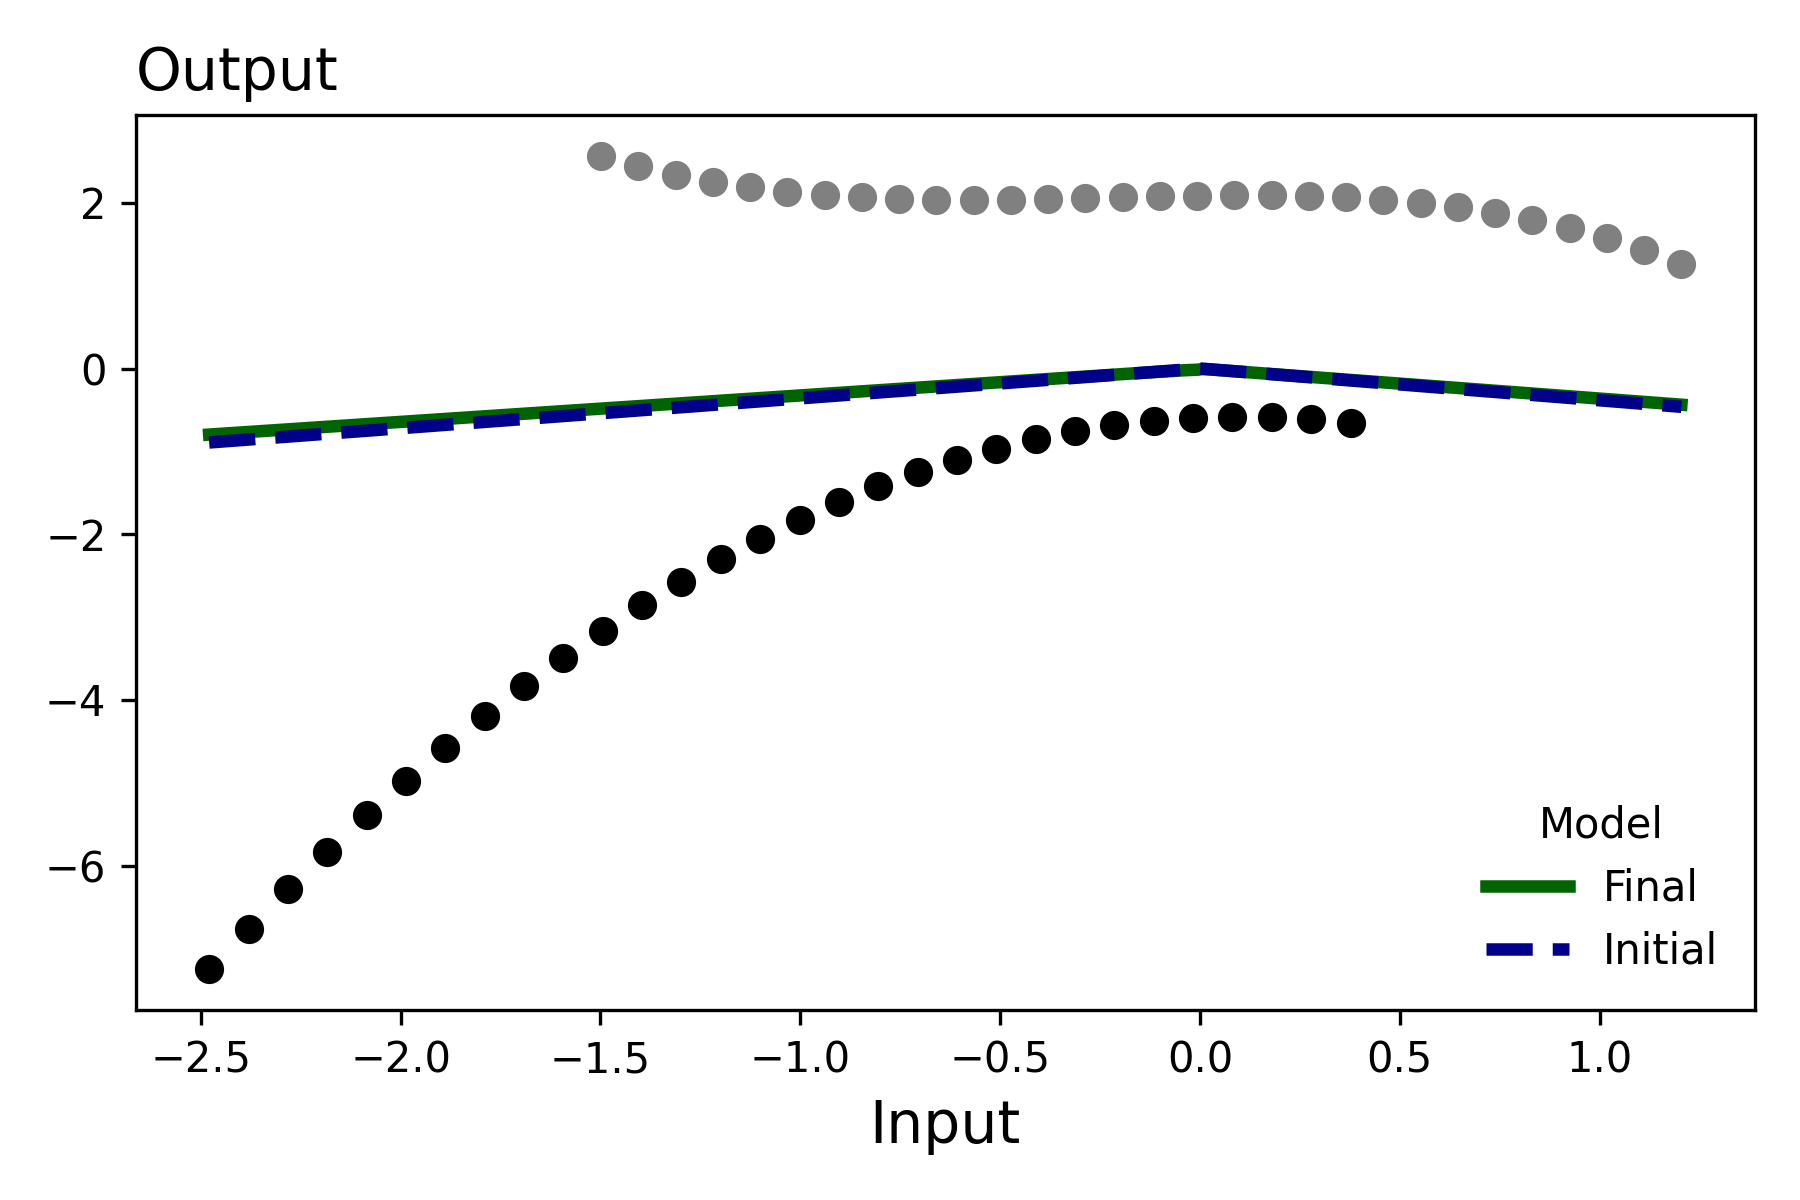
\includegraphics[width=.95\linewidth]{figures/framework/full_inner_loop_models.png}
    \caption{}
    %\label{SUBFIGURE LABEL 4}
\end{subfigure}
\caption{Without regularizing the implicit cluster maps, we risk losing the signal of the gradient -- \href{https://github.com/pharringtonp19/rfp/blob/main/notebooks/Missing_Gradients.ipynb}{Reproduced Here}}
\label{fig:Missinggrads}
\end{figure}
\subsection{Loss Function}
\begin{align*}
    \hat{\theta} &= \underset{\theta}{\textrm{argmin}}\ \mathcal{L}(\theta) \\ 
    &= \underset{\theta}{\textrm{argmin}}\ \sum _c \mathcal{L}_c(\theta)\\ 
    &= \underset{\theta}{\textrm{argmin}}\ \sum _c  F(\theta, \theta^*_c(\theta))\\
    &= \underset{\theta}{\textrm{argmin}}\ \sum _c  F(\theta, \underset{\theta_c}{\textrm{argmin}} \ F(\theta, \theta_c) )\\
\end{align*}
\subsection{Haskell-like Signatures}
\begin{align*} 
&\text{regMAML} :: \text{Data} \rightarrow \text{Params} \rightarrow \big(\textrm{Params}, \text{Float}\big) \\
&\text{regMAML} \ \textcolor{blue}{\text{data}} \ \textcolor{purple}{\theta} := \Big(\text{Update}_m \circ \text{Update}_{m-1} \dots \circ \text{Update}_1 \Big) \ \textcolor{purple}{\theta}, \quad \mathcal{L}_c(\textcolor{blue}{\text{data}}, \textcolor{purple}{\theta})  \\ 
&  \quad \quad \quad \quad \quad \quad \quad \quad \quad \quad \text{where} \quad  \text{Update}_t \  \theta = \theta - \alpha_t \nabla \mathcal{L}_c(\textcolor{blue}{\text{data}}, \textcolor{purple}{\theta})
\end{align*}
\begin{align*}
    &\text{regNeuralODE} :: \text{Data} \rightarrow \text{Params} \rightarrow \big(\textrm{Data}, \text{Float}\big) \\
&\text{regNeuralODE} \ \_ \ \textcolor{blue}{x} \ \_ \ \textcolor{purple}{\theta} := x + \int f(t, x(t), \theta)dt, \quad \int \Big\| \frac{\partial ^k}{dt^k}f(t, x(t), \theta) \Big\|dt \\ 
& \quad \quad \quad \quad \quad \quad \quad \quad \quad \quad \text{where}  \quad x(0)=x \\ \\ 
\end{align*}
\subsection{Method Implementation}
\begin{figure}[htbp]
\centering
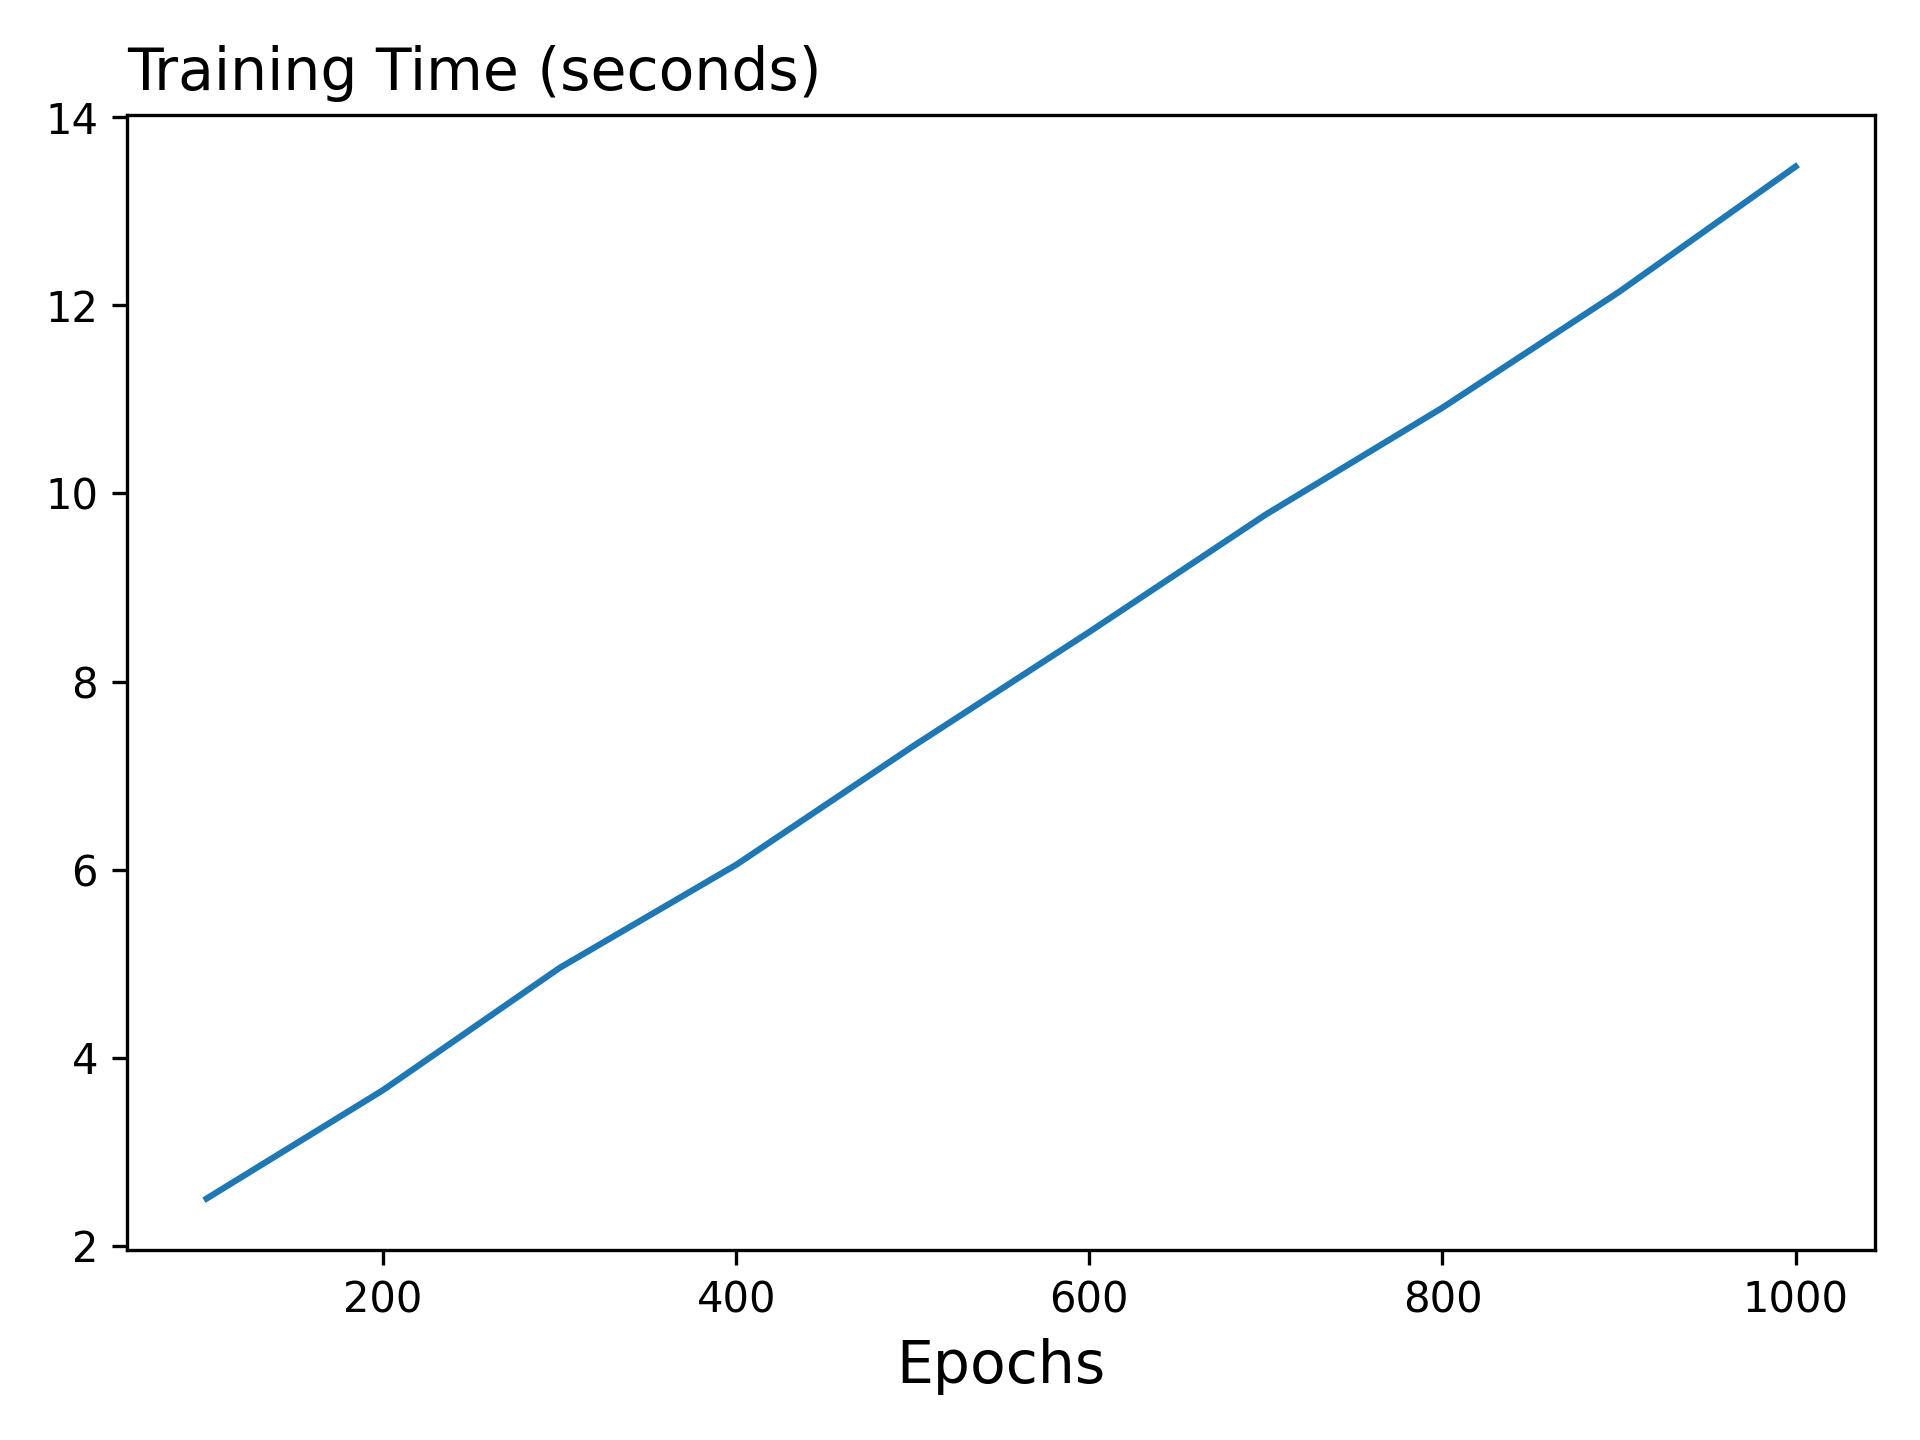
\includegraphics[width=.5\linewidth]{figures/framework/method_time.png}
\caption{ \href{https://github.com/pharringtonp19/evictions/blob/main/scripts/method/time_train_plot.py}{Reproduced Here}}
\label{FIGURE LABEL}
\end{figure}

\begin{figure}[htbp]
\centering
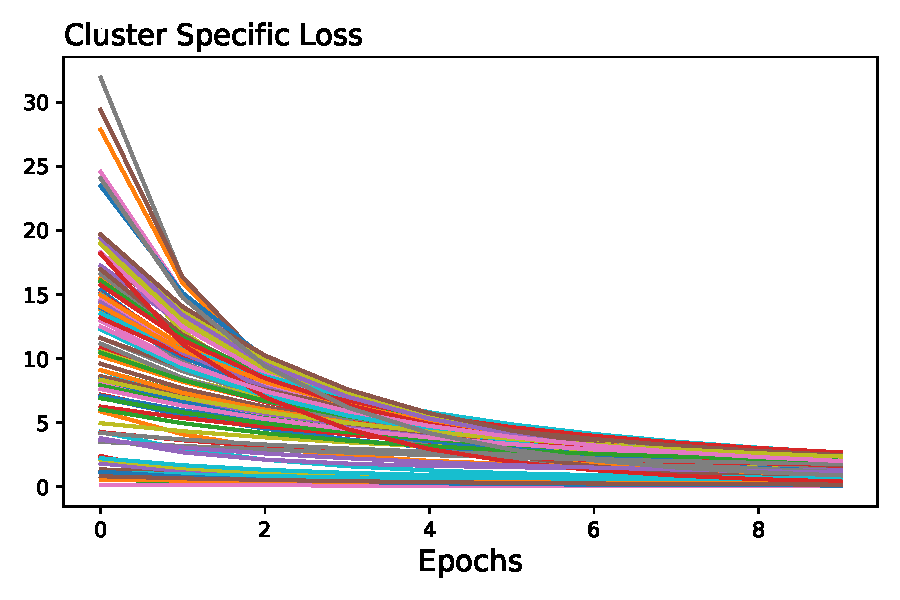
\includegraphics[width=.5\linewidth]{figures/framework/inner_loop_0.pdf}
\caption{ \href{https://github.com/pharringtonp19/evictions/blob/main/scripts/cceh/primary/diff_n_mean_rrh.py}{Reproduced Here}}
\label{FIGURE LABEL}
\end{figure}
Using individual level data from the U.S. Department of Housing and Urban Development, and fitting a variety of estimators to the data, from difference-in-means to machine learning based estimators, our preliminary estimates suggest while the policy has no noticeable effects on for the average individuals, it may make it more difficult for African American women to find permanent housing. The estimate, while crude and preliminary, maintains a positive sign above $5$ percentage points both across regression specifications as well as across subsets of zip codes. 
Eviction number from \cite{gromis2022estimating}. (Individual Costs): \cite{collinson2022eviction} writes, ``We find that eviction causes significant disruptions that are reflected in increases in residential mobility, homelessness, and hospital use''. (Court Costs): As \cite{seron2001impact} notes, legal representation actually might decrease housing court costs as the number of appearances and post judgement motions decline. (General Public): As \cite{desmond2019unaffordable} writes, ``Residential instability often brings about other forms of instability—in families, schools, communities— compromising the life chances of adults and children''

(Multitude of Causes):  David Ehrens writes in his \href{https://dartmouth.theweektoday.com/article/opinion-support-right-counsel-renters/58185}{letter} to the editor of \href{https://dartmouth.theweektoday.com/}{Dartmouth Week} of ``evictions related to the pandemic, chronic housing supply shortages, inequities in lending, generational poverty, and other harms''. (Eviction Proceedings): \textcolor{blue}{Missing Reference} writes ``the vast majority resolved by default or settlement, typically the result of hallway negotiation'' (Growing Interest): \cite{engler2010connecting} writes ``a renewed call for a civil right to counsel, or civil Gideon, has gained momentum \dots as well as a surge in membership in the newly-created National Coalition for a Civil Right to Counsel.''
\end{comment}
\end{document} 

